\documentclass[12pt,a4paper,twoside]{mwart}
\usepackage[T1]{fontenc}
\usepackage[utf8]{inputenc}
\usepackage[polish]{babel}
\usepackage{polski}
\usepackage{indentfirst}
\usepackage[left=3cm,right=2cm,top=2.5cm,bottom=2.5cm]{geometry}
\usepackage{todonotes}
\usepackage{listings}
\usepackage{float}
\usepackage{hyperref}
\usepackage{dirtree}
\usepackage{fancyhdr}
\usepackage[nottoc,numbib]{tocbibind}
\usepackage{enumitem}
\usepackage{csquotes}
\DeclareQuoteAlias{croatian}{polish}
\usepackage[maxbibnames=99]{biblatex}
\addbibresource{References.bib}
\usepackage{url}
\usepackage{amsmath}
\usepackage{hyphenat}
\usepackage{graphicx}
\usepackage{caption}
\usepackage{subcaption}
\captionsetup{compatibility=false}
%% \setlength{\parskip}{13pt plus 2pt minus 3pt} %% Odstęp dla paragrafów
%% \linespread{1.15} odstęp pomiędzy liniami?

\newcommand{\makecell}[2][@{}c@{}]{\begin{tabular}{#1}#2\end{tabular}}
\newcommand{\file}[1]{\textbf{\textit{\textcolor{darkgreen}{#1}}}}
\newcommand{\folder}[1]{\textbf{\textit{\textcolor{dodgerblue}{#1}}}}

\pagestyle{fancy}
%% JN: uproszczenie paginy: tylko autor i tytuł pracy, zamiast tytułu
%%     bieżącego rozdziału.
\renewcommand{\sectionmark}[1]{\markright{#1}}
\fancyhf{}

\fancyhead[LO]{\small \emph{\nouppercase{\rightmark}}}
\fancyhead[RE]{\small \emph{\nouppercase{\thesubsection}}}

\cfoot{\fancyplain{}{\thepage}}

% Część odpowiedzialna za styl kodu
% Taken from Lena Herrmann at 
% http://lenaherrmann.net/2010/05/20/javascript-syntax-highlighting-in-the-latex-listings-package
\usepackage{listings}
\usepackage{color}
\definecolor{lightgray}{rgb}{.9,.9,.9}
\definecolor{darkgray}{rgb}{.4,.4,.4}
\definecolor{purple}{rgb}{0.65, 0.12, 0.82}
\definecolor{dodgerblue}{RGB}{28, 134, 238}
\definecolor{darkgreen}{RGB}{0,153,51}
\definecolor{darkOrange}{RGB}{120,30,0}

\lstdefinelanguage{JavaScript}{
  keywords={typeof, new, true, false, catch, function, return, null, try, catch, switch, var, let, if, in, while, do, else, case, break},
  keywordstyle=\color{purple}\bfseries,
  ndkeywords={class, export, boolean, throw, implements, import, this, Math, Float32Array, Array},
  ndkeywordstyle=\color{blue}\bfseries,
  identifierstyle=\color{black},
  sensitive=false,
  comment=[l]{//},
  morecomment=[s]{/*}{*/},
  commentstyle=\color{darkgreen}\ttfamily,
  stringstyle=\color{darkOrange}\ttfamily,
  morestring=[b]',
  morestring=[b]"
}

\lstset{
   language=JavaScript,
   backgroundcolor=\color{lightgray},
   extendedchars=true,
   basicstyle=\footnotesize\ttfamily,
   showstringspaces=false,
   showspaces=false,
   numbers=left,
   numberstyle=\footnotesize,
   numbersep=9pt,
   tabsize=2,
   breaklines=true,
   showtabs=false,
   captionpos=b
}

\hyphenation{FORTRAN Wi-ki-books pow-szech-ną}
\setlength{\parindent}{4em}
\setlength {\marginparwidth }{2cm}
\setlength{\parskip}{0em} %odstęp pomiędzy paragrafami
\renewcommand{\baselinestretch}{1.5}
\captionsetup[figure]{labelfont=it,textfont={it}}
\captionsetup[table]{labelfont=it,textfont={it}}

\begin{document}

\begin{titlepage}
	\begin{center}
		\large Uniwersytet Mikołaja Kopernika w Toruniu\\
		\large Wydział Matematyki i Informatyki\\
		\vspace{3cm} 
		\large Patryk Bieszke\\
			nr albumu: 273187\\
			informatyka\\
		\vspace{2cm}
		Praca magisterska\\
	
		\vspace{2cm} 
		\huge Generowanie kompozycji muzycznych z użyciem sieci neuronowych\\
	\end{center}
	\hfill
	\begin{minipage}{6cm}
		\vspace{2cm}
		Opiekun pracy dyplomowej\\
		prof. dr hab. Piotr Wiśniewski
	\end{minipage}
	\vspace{3cm}
	\begin{center}
		Toruń 2019\\
	\end{center}
\end{titlepage}


\pagenumbering{gobble}% Remove page numbers (and reset to 1)

\clearpage
\thispagestyle{empty}
\mbox{}

\pagenumbering{arabic}
\tableofcontents 
\clearpage

\setcounter{secnumdepth}{0}
\section{Wstęp}
\label{sec:wstep}

\newpage

\section{Słownik skrótów}
\begin{itemize}
  \item \textbf{FT} - \textit{ang. \textbf{F}ourier \textbf{T}ransform}, pol. Transformata Fouriera
  \item \textbf{DFT} - \textit{ang. \textbf{D}iscrete \textbf{F}ourier \textbf{T}ransform}, pol. Dyskretna Transformata Fouriera
  \item \textbf{FFT} - \textit{ang. \textbf{F}ast \textbf{F}ourier \textbf{T}ransform}, pol. Szybka Transformata Fouriera
  \item \textbf{STFT} - \textit{ang. \textbf{S}hort- \textbf{T}ime \textbf{F}ourier \textbf{T}ransform}, pol. Krótkoczasowa Transformata Fouriera
  \item \textbf{DAW} - \textit{ang. \textbf{D}igital \textbf{A}udio \textbf{W}orkstation}, pol. Cyfrowa Stacja Robocza 
  \item \textbf{MIDI} - \textit{ang. \textbf{M}usical \textbf{I}nstrument \textbf{D}igital \textbf{I}nterface}, pol. Cyfrowy Interfejs Instrumentów Muzycznych
  \item \textbf{AUX} - \textit{ang. \textbf{Aux}iliary}
  \item \textbf{W3C} - \textit{ang. \textbf{W}orld \textbf{W}ide \textbf{W}eb \textbf{C}onsortium}
  \item \textbf{HTML} - \textit{ang. \textbf{H}yper\textbf{t}ext \textbf{M}arkup \textbf{L}anguage}
  \item \textbf{CSS} - \textit{ang.  \textbf{C}ascading \textbf{S}tyle \textbf{S}heets}
  \item \textbf{JS} - \textit{\textbf{J}ava\textbf{S}cript}
  \item \textbf{TS} - \textit{\textbf{T}ype\textbf{S}cript}
  \item \textbf{DOM} - \textit{ang. \textbf{D}ocument \textbf{O}bject \textbf{M}odel}
  \item \textbf{API} - \textit{ang. \textbf{A}pplication \textbf{P}rogramming \textbf{I}nterface}
  \item \textbf{CLI} - \textit{ang. \textbf{C}ommand \textbf{L}ine \textbf{I}nterface}
  \item \textbf{CQRS} - \textit{ang. \textbf{C}ommand \textbf{Q}uery \textbf{R}esponsibility \textbf{S}egregation}
  \item \textbf{URL} - \textit{ang. \textbf{U}niform \textbf{R}esource \textbf{L}ocator }
  \item \textbf{npm} - \textit{ang. \textbf{N}ode \textbf{P}ackage \textbf{M}anager}
  \item \textbf{IOI} - \textit{ang. \textbf{I}nter-\textbf{o}nset \textbf{i}nterval, pol. Odstęp pomiędzy początkami dźwięków}
  \item \textbf{TFR} - \textit{ang. \textbf{T}ime-\textbf{F}requency \textbf{R}epresentation, pol. Reprezentacja Czasu-Częstotliwości}
\end{itemize}
\newpage
\setcounter{secnumdepth}{4}

\section{Transkrypcja muzyki}
Sygnały akustyczne, przetworzone przez przetwornik analogowo-cyfrowy (A/C) są przechowywane są w postaci binarnych plików binarnych, których zawartością są sygnały foniczne w formie cyfrowej. Sygnały cyfrowe są sygnałami dyskretnymi czasu dyskretnego, które zostały poddane procesowi kwantowania wartości, przykładowo do najbliższych liczb całkowitych \cite[1-4]{CyfrowePrzetwarzanieSygnalowOdTeoriiDoZastosowan}. Sposób, w jaki pliki te przechowują dane jest zdeterminowany przez wiele parametrów, jak kodowanie, które zostało na nich zastosowane, częstotliwość próbkowania, ilość kanałów itp. Istnieje wiele kodowań przeznaczonych do danych dźwiękowych, zarówno nieskompresowanych jak i skompresowanych. Te drugie powstały z myślą o zaoszczędzeniu jak największej ilości pamięci w znaleźć od tego, w jakim stopniu można pójść na kompromis z jakością skompresowanego sygnału \cite[66]{Homerecording:DlaKazdego}. Częstotliwość próbkowania ma również znaczący wpływ na wynikowy rozmiar plików, jak i ilość bitów przeznaczony na pojedyńczy sampel. Wszystkie cechy jakie posiada cyfrowa reprezentacja rzeczywistego dźwięku muszą być wzięte pod uwagę podczas jej przetwarzania.

W kontekście algorytmów generujących muzykę, binarne pliki dźwiękowe nie posiadają efektywnej struktury pozwalającej na trzymanie akustycznych informacji o melodii czy rytmice. Cechy, które można wydobyć ze zdigitalizowanego strumienia audio mogą posłużyć za istotne wskaźniki przy klasyfikacji zbiorów, natomiast kluczowe informacje odnoszące się do struktury kompozycji i harmonii poszczególnych sekcji szukać należy w transkrypcji danego utworu. 

%% z PWN : transkrypcja [łac. transcriptio ‘przepisywanie’], muz. opracowanie utworu muz. na inny niż w oryginale zespół wykonawczy (orkiestracja) lub inny instrument; Pytanie czy rozszerzenie tego znaczenia w języku polskim jest poprawne? także zapisanie utworu inną notacją muz.; transkrybować — zapisywać znakami współcz. notacji muz. utwory zapisane dawnymi systemami notacyjnymi, np. notacją modalną, menzuralną. Po ENG transkrypcja jest zgodna z rozdziałem

\textbf{Transkrypcja muzyki} to proces polegający na zapisaniu danego utworu muzycznego w sposób formalny, taki jak zapis nutowy, z istniejącego zapisu dźwiękowego. Operacja ta wykorzystywana jest do lepszego zrozumienia muzyki i możliwości jej wiernego odtworzenia. Algorytmiczne podejście do tego problemu obejmuje rozpoznanie rytmu i wysokości tonu poprzez analizę zdigitalizowanego sygnału fonicznego. Do zadań tego procesu często zalicza się odseparowanie od siebie poszczególnych instrumentów w danym utworze muzycznym, ponieważ nakładanie się na siebie sygnały odrębnych źródeł stanowi jeden z większych trudności transkrypcji.

Pierwsze próby zautomatyzowania procesu transkrypcji muzyki monofonicznej datowane są na lata 60. XX wieku. Bernard Gold w roku 1962 opublikował wypracowanie pod tytułem "Program komputerowy do wydobywania wysokości dźwięku" \cite{Transcription:Gold:ComputerProgramForPitchExtraction}. Pierwsze próby transkrypcji muzyki polifonicznej odbyły się w latach siedemdziesiątych, kiedy Moorer zaproponował system transkrypcji dwóch głosów \cite{Transcription:Moorer:SegmentationAndAnalysis}\cite{Transcription:Moorer:OnTheTranscriptionOfMusicalSOundByComputer}. We wszystkich wczesnych pracach naukowych nad tą tematyką liczba równoległych dźwięków była zawsze ograniczana do maksymalnie dwóch, jak i relacja pomiędzy wysokościami miała duże obostrzenia. Prace te były zorientowane na analizę tonu wokalnego w kontekście analizy mowy. Dla przykładu, praca \cite{Transcription:Gold:ComputerProgramForPitchExtraction} była napisana z myślą o urządzeniu zdolnym syntezować dźwięk mowy (tzw. vocoder). Metodologie używane do transkrypcji muzyki swoje fundamenty biorą właśnie z algorytmów analizujących mowę, które to były rozwijane w znacznie większym tempie w porównaniu do tych badających muzykę. W pracy Goto i Muraoka z roku 1994 \cite{Transcription::FirstRythm} po raz pierwszy pojawia się metoda do śledzenia rytmu w utworze muzycznym. Pierwsze próby transkrypcji instrumentów perkusyjnych odbyły się w latach 80 XX wieku w pracach naukowych \cite{Transcription:Schloss:AutomaticTranscriptionOfPercussiveMusic} i \cite{Transcription:Bilmes:TimingIsOfTHeEssence} \cite[6]{Transcription:Anssi:SignalProcessingMethods}.

Kompletna transkrypcja wymagała by dokładnej analizy wysokości dźwięków, czasów ich występowania i rodzaju instrumentu, przy pomocy którego dane dźwięki zostały wygenerowane. Z racji tego, że złożoność tego zadania jest bardzo duża, a w niektórych przypadkach nawet teoretycznie niemożliwa, celem tak zwanej kompletnej transkrypcji jest wykrycie jak największej ilości składowych jak jest to możliwe. Terminem częściowej transkrypcji nazywa się znajdowanie dobrze zdefiniowanych części muzycznego sygnału, jak główna melodia i perkusja \cite[3-7]{Transcription:Anssi:SignalProcessingMethods}.

Najnowsze dokonania w dziedzinie automatycznej transkrypcji muzycznej są jednak nadal gorsze w rezultatach od profesjonalistów w dziedzinie muzyki. Rozwiązanie, które dawałoby rzetelne rezultaty w ogólnym zastosowaniu na muzyce jeszcze nie istnieje. Jednakże, z odpowiednimi założeniami co do sygnału źródłowego, najnowsze metody potrafią dokonać kompletnej transkrypcji utworu muzycznego. Restrykcje w analizowanym sygnale często sprowadzają się do ograniczenia polifoniczności (ilości jednoczesnych dźwięków) \cite{Transcription:BayesianHarmonicModels}, użycia tylko konkretnego instrumentu \cite{Transcription:Hawthorne:OnsetsAndFrames} czy braku interferencji z dźwiękami perkusyjnymi \cite{Transcription:Kameoka:HarmonicSeparation}.

Bez automatyzacji procesu, transkrypcja wykonywana manualnie zakładała profesjonalną wiedzę słuchacza, który iteracyjnie odsłuchując dany utwór ustala grane instrumenty wraz z częstotliwością fundamentalną lub akordem, która jest na nich grany. Wymusza to osobie transkrybującej wyróżnienie poszczególnych granych dźwięków, wyodrębniając jego długość, wysokość i korelacje do pozostałych granych dźwięków. Ludzkie ucho postrzega dźwięk relatywnie, co powoduje, że dużo łatwiej jest porównywać dźwięki niż je analizować w odizolowaniu, toteż referencyjne dźwięki, jak na przykład skala zagrana na pianinie, są często wykorzystywane przy tradycyjnym przebiegu procesu transkrypcji. W rezultacie zadanie to jest skomplikowane i wymaga dużego nakładu czasowego nawet dla profesjonalistów z doświadczeniem w dziedzinie muzykologii.

W tym rozdziale przedstawiony jest wciąż nierozwiązany problem automatycznej transkrypcji muzycznej, nakreślając najbardziej problematyczne rejony w oparciu o przykłady już istniejących rozwiązań.  Celem tych rozważań było przybliżenie ogólnej koncepcji transkrypcji muzycznej, teorii na jakiej się opierają, \todo[inline]{Move somewhere}oraz próba zoptymalizowania części z nich poprzez zrównoleglenie obliczeń wykorzystując kartę graficzną.

\subsection{Jak "działa" muzyka}\label{sec:JakDzialaMuzyka}
Przed dalszymi rozważaniami istotne jest zdefiniowanie terminologii związanej z muzyką jak i samej muzyki. Muzyka, równoznaczne z utworem muzycznym, jest uporządkowanym zbiory dźwięków o odpowiednich wysokościach i głośnościach z zachowaniem odpowiedniego rytmu. Wysokości tych dźwięków są proporcjonalne do częstotliwości wibracji, które zostały wytworzone przez dany instrument lub głos ludzki. Głośność określana jest przy pomocy amplitudy zadanego sygnału akustycznego. Starając się rozłożyć skomplikowaną strukturę utworów muzycznych na rozdzielne części, można wyróżnić cztery rozdzielne składowe, których zbadanie i zinterpretowanie jest przedmiotem algorytmów transkrypcji muzycznej. Są to:
\begin{itemize}
\item Rytm
\item Wysokość tonu
\item Głośność
\item Barwa dźwięku
\end{itemize}
Zapis nutowy utworu jest zdefiniowany w taki sposób, że wszystkie wyżej wymienione cechy są jednoznacznie opisane, z kolei ten jest wystarczającym źródłem informacji dla muzyków aby zagrać dany utwór muzyczny. Zapisane nuty przedstawiają wysokość tonu wraz z długością granego dźwięku i poziomem głośności jaki powinien zostać zastosowany. Jego barwę reprezentuje instrument muzyczny do którego odnosi się dany zapis nutowy, toteż nie jest ona rozpisana w dosłownym zapisie nutowym.

Klucz w którym został napisany utwór, opisujący harmoniczną podstawę kompozycji jest również bardzo istotną informacją, która dostępna jest na podstawie zapisu nutowego. W praktyce klucz ogranicza dostępne wysokości tonu jakie mogą być zagrane. Wiele kompozycji muzycznych dynamicznie manipuluje kluczem, tworząc mniej statyczne linie melodyczne, co uniemożliwia opieranie transkrypcji o ten parametr.

Zapis nutowy zawiera też informacje o tempie utworu, czyli szybkość z jaką kolejne dźwięki powinny być grane, jak i sygnaturę czasową, która wyznacza bazową strukturę rytmiczną w jakiej dany utwór został napisany. Te dwie informacje składają się na wylistowany wyżej rytm.

Informacją, którą zapis nutowy nie dostarcza jawnie, jest barwa dźwięku. Parametr ten jest ściśle związany z instrumentem, którego dotyczy dany dźwięk. Każde ze źródeł dźwięku cechuje się odrębną barwą, nawet gdy uwzględnić taką samą wysokość i głośność sygnału fonicznego. Problem rozróżniania tej cechy jest związany nie tylko z transkrypcją muzyki, ale i algorytmami identyfikującymi instrumenty poprzez analizę barwy dźwięku.

W dalszej kolejności zostaną pokrótce opisane cztery wymienione wyżej cechy, które są głównym przedmiotem analizy w kierunku transkrypcji muzycznej \cite[63]{Homerecording:DlaKazdego}.
\begin{figure}[H]
  \begin{center}
    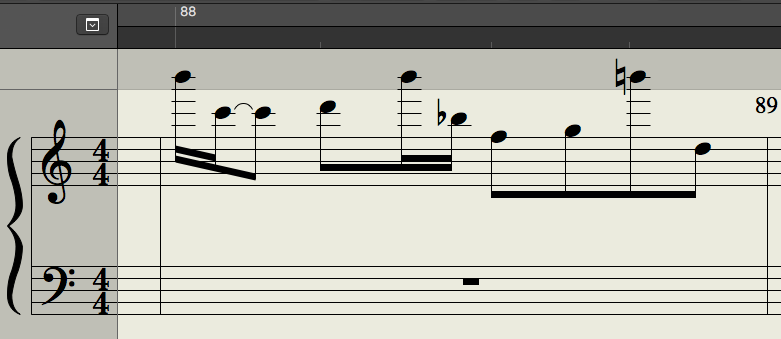
\includegraphics[scale=0.5]{images/pieciolinia_logic.png}
    \caption{Przykład notacji muzycznej wygenerowanej z pliku MIDI w programie Logic Pro X. Widać na nim takie informacje jak metrum czy wysokości i długości granych dźwięków}
  \end{center}
\end{figure}

\subsubsection{Rytm}


W kontekście muzykologii, rytm jest relacją czasową pomiędzy poszczególnymi dźwiękami, tworzącą strukturę rytmiczną utworu. Nie można niestety zakładać stałości rytmu na przestrzeni całej kompozycji, ponieważ powszechną praktyką kompozytorów jest jego modyfikacja na przestrzeni piosenki w celu uzyskania konkretnych efektów artystycznych. Dla przykładu, minimalne podnoszenie tempa na czas każdego z refrenów jest powszechnie stosowane w muzyce popularnej.

Informacja o rytmie jest zapisana w relacjach pomiędzy poszczególnymi dźwiękami i pomiędzy większymi strukturami wewnątrz utworu. \textbf{Odstęp pomiędzy początkami dźwięków} (\textit{ang. Inter-onset interval, IOI}) pełni bardzo istotną rolę w rytmice utworu, jak i strukturze perkusyjnej. Pojęcie to odnosi się do interwału czasowego pomiędzy dwoma początkami dźwięków (np. moment uderzenia w werbel), która to cecha jest dużo bardziej istotna w rytmice niż długość danych dźwięków. \cite[473-500]{Transcription:Clarke:RhythmAndTiming}

Podstawową jednostką rytmiczną jest nuta. Miarą tempa utworu przeniesioną na domenę fizyczną są \textbf{uderzenia na minutę} \textit{(ang. beats per minute, BPM)} oznaczające liczbę ćwierćnut (beatów) przypadających na jedną minutę. \textbf{Taktem} nazywamy odcinek zapisu muzycznego wizualnie oznaczony pionowymi kreskami. Takty tworzą regularne odcinki czasowe, a ich długość jest zależna od \textbf{metrum}. Metrum jest oznaczeniem metrycznym opisującym ile jakich jednostek mieści się w takcie. Dla przykładu, najpopularniejszym metrum w muzyce pop jest 4/4, co oznacza, że w każdym takcie mieszczą się cztery ćwierć nuty.

\begin{figure}[H]
  \begin{center}
    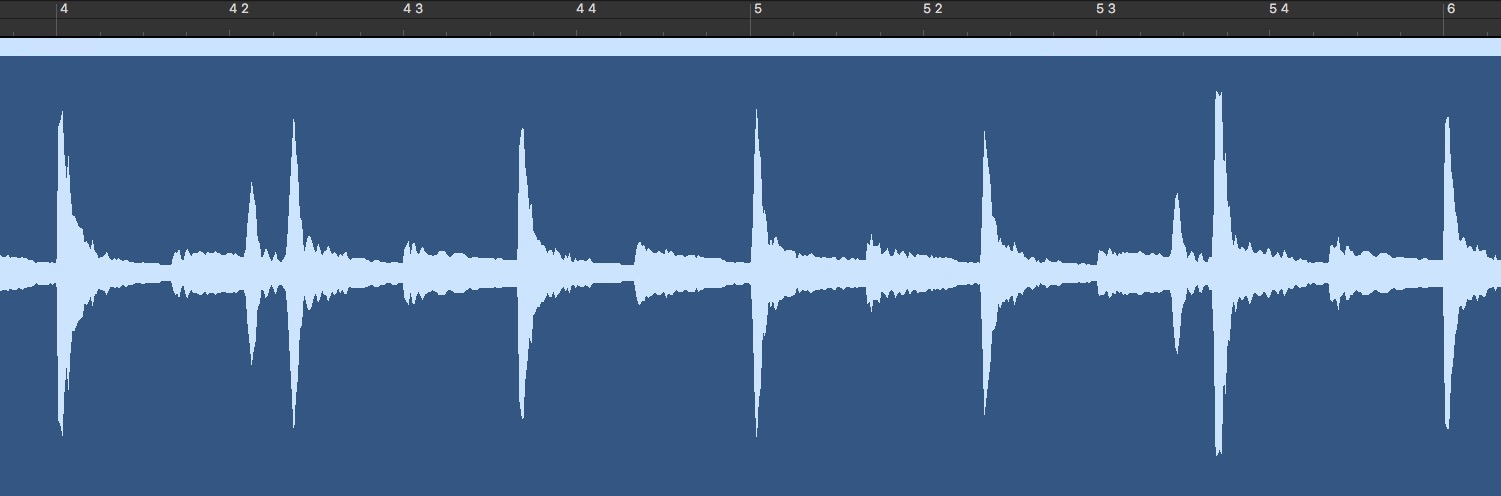
\includegraphics[scale=0.3]{images/RythmMertic.jpg}
    \caption{Sygnał akustyczny z wyraźnymi metrykami muzycznymi. Na osi poziomej liczbowo oznaczona jest metryka nutowa (4 beaty), mniejszymi zaś regularne odstępy taktowe.}
    \label{fig:rythmMertic}
  \end{center}
\end{figure}

Zbadanie rytmiki wymaga wyznaczenia metrum i długości poszczególnych jednostek metrycznych utworu. Ze względu na to, że nagrania muzyczne cechują się periodycznością wokół tych jednostek, wykrycie wzorca regularnych, przeplatanych zestresowanych i nieakcentowanych uderzeń (często nazywanych słabszymi i silniejszymi) \cite[12-35]{Transcription:Lerdahl:GenerativeTheory}. Pozyskane \textit{pulsy} o różnych czasowych poziomach razem tworzą strukturę rytmiczna. Przykład takiej struktury przedstawiony jest na rysunku \ref{fig:rythmMertic}, który przedstawia sygnał nagranej perkusji. W równych odstępach pojawiające się piki oznaczają stopkę, werbel oraz talerze, każde występują periodycznie.

W skład rytmu wchodzi również \textbf{grupowanie}. Termin ten odwołuje się do powiązań pomiędzy pojedyńczymi dźwiękami, które razem tworzą łączną frazy, a te z kolei dalej grupowane tworzą większe i bardziej złożone jednostki w hierarchicznej strukturze \cite[12-35]{Transcription:Lerdahl:GenerativeTheory}. 

\subsubsection{Wysokość tonu}\label{subsec:pitch}

Wysokość tonu, czy też wysokość dźwięku, jest percepcyjnym atrybutem za pomocą którego porządkowane są dźwięki na skali częstotliwości, od najniższych do najwyższych. Jest to pojęcie tożsame z częstotliwością sygnału sinusoidalnego zgodnego z tym, które jest odebrane przez ludzkie ucho \cite[3491-3502]{Transcription:Hartmann:PitchPeriodicityAuditoryOrganization}. 

\begin{figure}[H]
  \begin{center}
    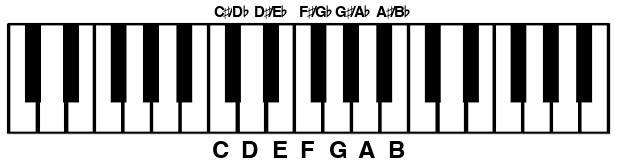
\includegraphics[scale=0.5]{images/PianoRoll.png}
    \caption{Ilustracja przedstawiająca trzy oktawy klawiatury pianina z oznaczonymi muzycznymi nazwami nut}
    \label{fig:pianoRoll}
  \end{center}
\end{figure}

\textbf{Częstotliwość fundamentalna} (w dalszej części oznaczana jako \textbf{F0}) jest terminem fizycznym dla sygnałów okresowych i prawie okresowych zdefiniowany jako odwrotność długości okresu sygnału. W niejednoznacznych przypadkach F0 określony jest jako okres odpowiadający postrzeganej wysokości tonu \cite[8]{Transcription:Anssi:SignalProcessingMethods}.

F0 jest ściśle powiązana z wysokością tonu. Współczesna muzyka zachodnia opera się na \textbf{skali melowej}. System równomiernie kwantuje nuty na logarytmicznej skali spektrum częstotliwości na tak zwane półtony, czyli najmniejsze interwały. Każda z tak powstałych muzycznych nut ma przypisaną literę w celu odróżnienia, alfabetycznie od A do G wraz razem z podwyższeniami (moll, w języku angielski \textit{sharp} oznaczany symbolem $\sharp$) i obniżeniami (dur, w języku angielskim \textit{flat} oznaczany symbolem $\flat$) półtonowymi. Tak nazwane wysokości są grupowane w oktawy, z których każda zawierająca 12 półtonów. Pełna nazwa granego dźwięku powinna zawierać nazwę literalną wraz z numerem oktawy. Ze względu na tak skonstruowany system nazewnictwa, niektóre z dźwięków mogą mieć dwie poprawne nazwy (np. A$\sharp$4 i B$\flat$4). O tym, którą z tych dwóch nazw należy użyć, zazwyczaj zależy konwencja którą używa kompozytor.

Omówiony system zakłada referencyjne mierzenie częstotliwości zależnie od wysokości A4, która powinna być równa 440 Hz. Każda podwyższenie oktawy powinno powodować dwukrotne zwiększenie sie częstotliwości fundamentalnej. Standard MIDI mapuje daną częstotliwością bazową na liczbę rzeczywistą odpowiadającą wysokości dźwięku przy pomocy wzoru \cite[67-71]{Homerecording:LevelUp}:
\begin{equation} \label{eq:midi_freq}
p = 69 + 12 * \log{2}(\frac{f}{440 Hz})
\end{equation}

Istnieją oczywiście instrumenty, które generują dźwięki o dowolnych F0, a nie jedynie dyskretne wartości, jak na przykład skrzypce. Kwantyzacja jest procesem który tak powstałe dźwięki skategoryzuje do najbliższej wartości w sensie częstotliwości nazwanych nut, dzięki czemu można je formalnie zapisać w procesie transkrypcji \cite{Transcription:Burns:InversalScalesTuning}.

Ciekawą własnością niemalże wszystkich kultur muzycznych jest podobieństwo do siebie odpowiednich nut w oktawach. Nuty A2, A3 i A4 dla przykładu mają taką samą rolę w kontekście harmoniczności. Brzmią one bardzo podobnie do siebie, jedynie różnią się wysokością. Ze względu na tą cechę, opisany wyżej system redukuje liczbę wszystkich istniejących dźwięków do jedynie 12 klas dźwięków, po 1 na każdą z nut w oktawie. Korzystając ze wzoru ~\ref{eq:midi_freq} dla wielokrotności liczby 440 można uzyskać tabelkę z częstotliwościami dźwięków \textbf{A} w kolejnych oktawach, jak w tabeli \ref{tab:FqMidi}.

\begin{table}[ht]
  \begin{center}
    \begin{tabular}{ |c|c|c| } 
    \hline
    p & f & Literalna nazwa wysokości dźwięku\\
    \hline
    33 & 55 & A1\\
    45 & 110 & A2\\
    57 & 220 & A3\\
    69 & 440 & A4\\
    81 & 880 & A5\\
    93 & 1760 & A6\\
    105 & 3520 & A7\\
    \hline
    \end{tabular}
  \end{center}
  \caption{Wysokości kolejnych dźwięków A zgodna ze wzorem ~\ref{eq:midi_freq}}
  \label{tab:FqMidi}
\end{table}

Relacja pomiędzy wysokościami używanych tonów jest ważną informacją przy analizie muzycznej. Mimo dużej ilości możliwych częstotliwości, używane nuty często ograniczane są do podzbiorów według tak zwanych kluczy. Badając rozkład częstotliwości takie informacje mogą znacznie ograniczyć błędy podczas badania sygnału. Należy jednak mieć na uwadze fakt, że nagrany instrument może nie posiadać dokładnie takiej samej częstotliwości jak oczekiwana dla danej wysokości tonu ze względu na charakterystykę instrumentu czy też techniczne parametry nagrania. Dodatkowym utrudnieniem są skale które bazują na innych niż zachodnich systemach dobierania wysokości. W tej pracy badane będą jedynie utwory bazujące na wyżej opisanym systemie, jednak na uwadzę należy mieć fakt, że nie jest to uniwersalne rozwiązanie. Również z artystycznych względów docelowe częstotliwości generowane przez instrumenty odbiegają od tych przewidzianych przez opisany system. Nieharmoniczność najczęściej ustala się na poziomie 5\%, lecz nie istnieje sformalizowany zakres. Próba rozpoznawania jedynie konkretnych częstotliwości tonów mogło by być dużym uproszczeniem w analizie sygnałów fonicznych, lecz jednocześnie znacząco ograniczyłby jej uniwersalność \cite[64-65]{Homerecording:DlaKazdego} \cite[7-11]{Transcription:Anssi:SignalProcessingMethods}.

\subsubsection{Głośność}
Termin głośności z reguły nie odnosi się do pojedyńczych nut, ale do większych sekcji. W notacji muzycznej nie często używa się słowa "głośność". To co słuchacz odbiera jako siłę dźwięku z punktu widzenia muzyka jest dynamiką granego fragmentu. Większość instrumentów używanych do tworzenia muzyki posiada zdolność wytworzenia zróżnicowanych w sile fal akustycznych. Podstawą skali dynamiki są dwa słowa kluczowe:

\begin{itemize}
  \item \textbf{f} (forte) - głośno
  \item \textbf{p} (piano) - cicho
\end{itemize}

Pomiędzy wymienionymi stopniami istnieją kroki pośrednie, odpowiednio mezzo\-forte (dość głośno) i mezzo-piano (dość cicho). Poza czterema wymienionymi przypadkami dostępne są również skrajności odpowiadające za bardzo głośny (odpowiednio - cichy) i możliwie najgłośniejszy (odpowiednio - najcichszy) odcień dynamiki.

Z punktu widzenia algorytmicznej analizy muzyki problematyczne są dynamiki zwane crescendo i diminuendo. Odpowiadają one za kolejno stopniowe wzmacnianie i stopniowe osłabianie natężenia dynamiki. Łatwo jest pomylić takie zabiegi z innymi cechami sygnału audio.

Warto też wspomnieć o technice zwanej \textit{tremolo}, która określa artykulacje  grania wielu dźwięków o tej samej wysokości z różną dynamiką. Analizując sygnał łatwo jest pomylić kolejne uderzenia tremolo z zagraniem nowych nut.

Z praktycznego punktu widzenia głośność w plikach muzycznych jest zdeterminowana przez to, jak dany utwór został wyprodukowany. W procesie nagrywania ogromne znaczenia ma położenie i rodzaj mikrofonu, jak i otoczenie w którym rejestrowany jest dźwięk. Mikrofony posiadają różne pasma przenoszenia i charakterystyki kierunkowe, które nie tylko mogą zniekształcić głośność nagrywanego instrumentu, ale również jego barwę. Różne rodzaje mikrofonów są wykorzystywane przy różnych źródłach dźwięku, np. mikrofony pojemnościowe są odpowiedniejsze do nagrywania wokali i instrumentów akustycznych niż wstęgowe, ponieważ przenoszą częstotliwości tych właśnie źródeł bardziej wiarygodnie \cite[48-52]{Homerecording:DlaKazdego}. Charakterystyka niektórych powierzchni może sprawić, że fałszywie cichsze częstotliwości będą wychodziły na przód nagrania. Mocna kompresja dynamiki utworu jest powszechna praktyką podczas procesu miksowania i masterowania utworów. Dzieje się tak, ponieważ ludzie impulsywnie uważają głośniejsze utwory za lepsze, co doprowadziło rynek muzyczny do produkowania utworów o niemal stałej dynamice głośności, co mogło graniczyć z białym szumem. Choć temat ten jest w trakcie regulacji, przez między innymi wprowadzenie ograniczeń dynamiki na podstawie jednostki LUFS danego utworu, dokładne analizowanie głośności wielu istniejących nagrań może doprowadzić do nieprawdziwych wniosków.

\begin{figure}[H]
  \begin{center}
    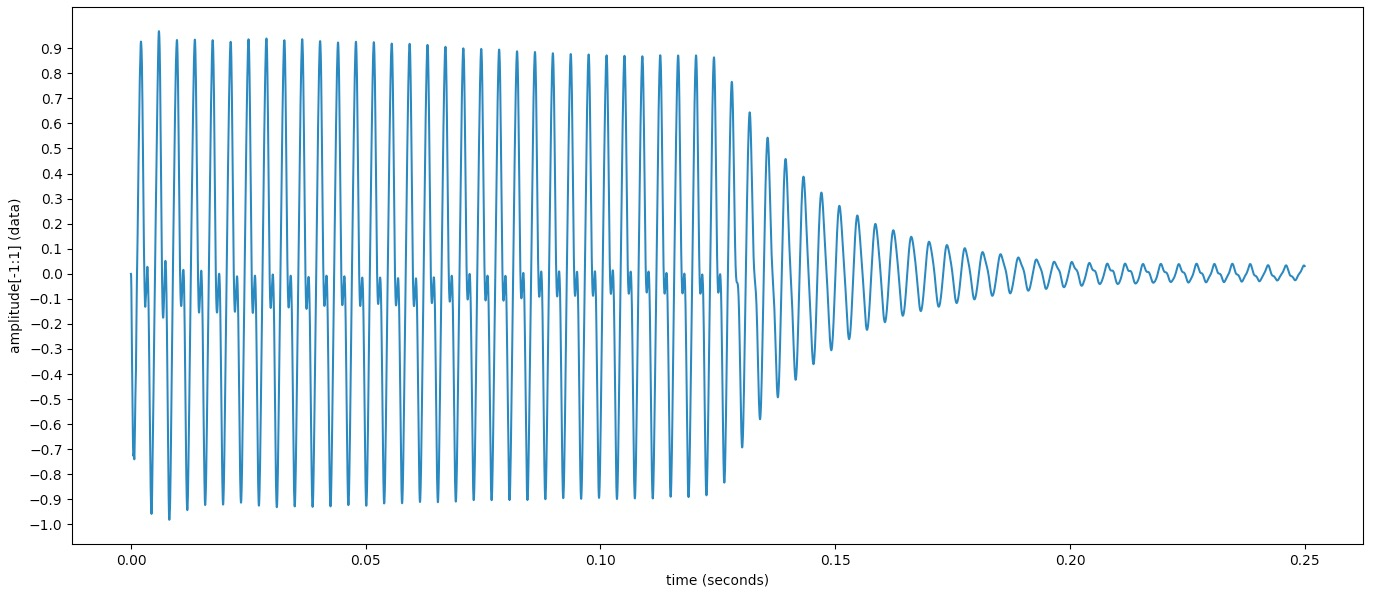
\includegraphics[scale=0.32]{images/Amplitude.jpg}
    \caption{Wykres przedstawiający sygnał dźwięku o zmiennej amplitudzie (głośności) względem czasu wygenerowany przez klasyczne pianino elektryczne.}
    \label{fig:amplitude}
  \end{center}
\end{figure}

\subsubsection{Barwa dźwięku}\label{sec:barwaDzwieku}
Barwa dźwięku (inaczej tembr) jest cechą odwołującą się do harmonicznej domeny sygnału fonicznego. Pozwala ona na odróżnienie od siebie dźwięków o tej samej głośności i wysokości granych na różnych instrumentach. Silne tony harmoniczne danej barwy sprawiają, że dźwięk jest bardziej wyrazisty. W przeciwnym wypadku, gdy siła tonów harmonicznych jest mała, sygnał staje się bardziej rozmyty dla odbiorcy. Barwa dźwięku jest zależna od amplitudy poszczególnych tonów harmonicznych, ich rozkładu w widmie jak i samej struktury tego widma. Jest to dobrze widoczne na rysunku \ref{fig:spektrogram}.

\begin{figure}[t]
  \begin{center}
  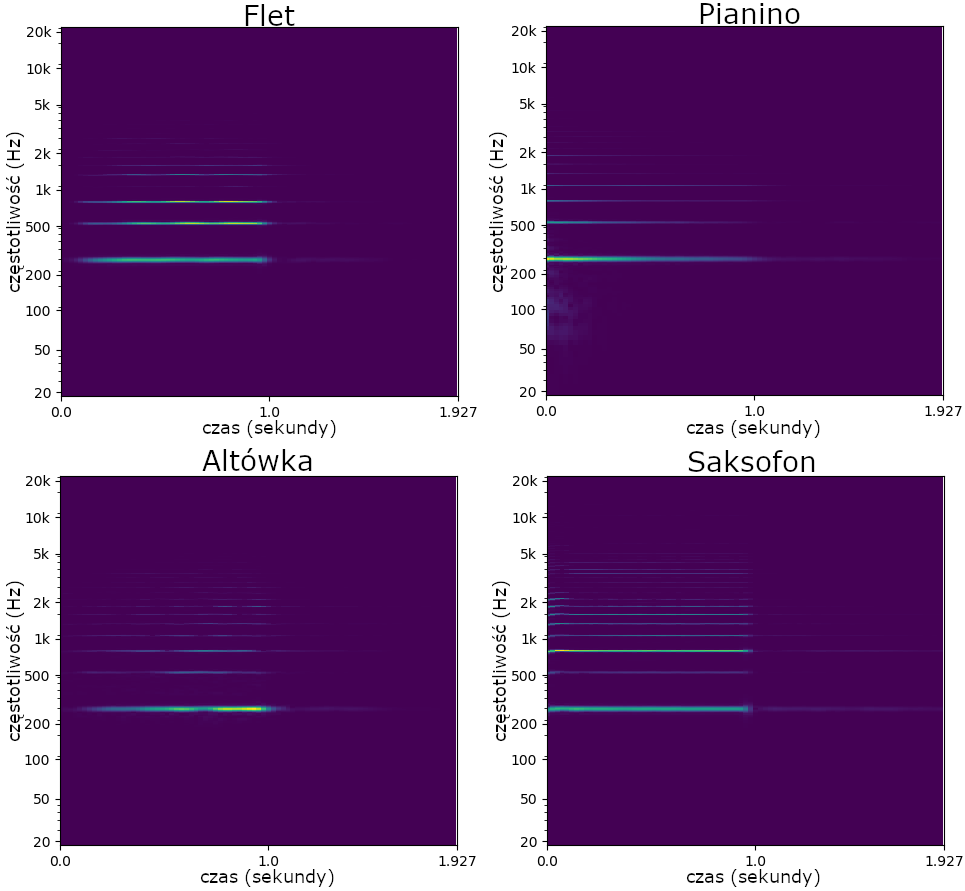
\includegraphics[scale=0.4]{images/spectogram_instruments.png}\\
  \caption{Spektrogramy dźwięku C3 (130.81Hz) grane na czterech różnych instrumentach (flet, pianino, altówka i saksofon) pokazują różnice w ilości i rozmieszczeniu harmonicznych każdego z dźwięków. Spektrogramy wykonane z 4096 samplami na okno, odstępem okien 1024 sampli i funkcją okna Hanna}
  \label{fig:spektrogram}
  \end{center}
\end{figure}

Ułożenie tonów harmonicznych jest zintegrowane z harmonią pomiędzy różnymi granymi nutami. Gdy dwa dźwięki są grane w tym samym czasie, nakładające się na siebie harmoniczne sprawiają, że dźwięk brzmi pozornie spójnie. Generuje to dodatkowe komplikacje dla algorytmów wykrywających wysokość tonów, które muszą odseparować nakładające się na siebie nuty.

Barwa dźwięku nie jest stała w czasie. Harmoniczne o wysokich częstotliwościach szybciej cichną w porównaniu do tych o niższych. Powoduje to, że nie tylko ogólna głośność jest mniejsza, ale i barwa ulega modyfikacji. Dla instrumentów dętych czy skrzypiec cechy jak wysokość tonu, głośność i barwa pozostają relatywnie stałe przez cały okres grania nuty, natomiast dźwięk pianina rozmywa się w czasie. Ta cecha barwy dźwięku musi zostać zaadresowana przy próbie dokładnej analizy sygnału fonicznego \cite[64-65]{Homerecording:DlaKazdego} \cite[804–816]{Transcription:Klapuri:MultipleFundamentalFrequencyEstimation}.

Istotnym pojęciem przy omawianiu barwy dźwięku jest \textbf{formant}. Formantem nazywane jest pasmo częstotliwości, w którego obrębie częstotliwości harmoniczne są wzmocnione względem pozostałych częstotliwości danego sygnału. Formanty mogą sprawić, że harmoniczne będą miały większą amplitudę niż częstotliwość fundamentalna. Istnienie tego zjawiska fonicznego uniemożliwia poprawność podejścia, w którym jako częstotliwość fundamentalna wybierana była by ta, o największej amplitudzie w analizowanym oknie \cite[62-63]{BarwaDzwieku:Formant}.
%%\todo[inline]{Czy mogę użyć książki której nawet nie mogę znależć on-line tylko jako referencja w innej pozycji? Który ISBN powinienem podawać, ISBN-10 czy ISBN-13? Czy istnieje jakiś stylesheet którego powinienem się trzymać? Kiedy boldować wyrazy a kiedy pisac kursywą? Bibliografia - czy może byc "and" pomiędzy autorami? Wykres analizy częstotliwościowej z innej książki przyciołem o jeden wykres żeby nie zajmował tyle miejsca, czy tak można?}

\subsection{Modelowanie systemu transkrypcji}
Muzyka jako ogół cech, jak i pojedyńczy utwór muzyczny posiadają bardzo wiele własności na podstawie których można opierać analizę. W celu zoptymalizowania algorytmu automatycznej transkrypcji należy przefiltrować wszystkie te dane i zdecydować się, które uznać za istotne, a które można uznać za zaniedbywalne. Strukturyzacja algorytmu i dobór reprezentacji danych jest równie istotna przy projektowaniu algorytmu.

Neuropsychologiczne badania, które były prowadzone w kontekście przetwarzania muzyki przez ludzki umysł dowodzą, że analiza dźwięku jest dzielona na pod-zadania. Pewne własności muzyki są odseparowywane od reszty bez szerszej perspektywy. Daje to informacje o tym, że modularyzacja podejścia do transkrypcji może być właściwym rozwiązaniem tego problemu. W automatycznej transkrypcji muzyki często używa się innych reprezentacji danych do analizy wysokości dźwięku, w których większy nacisk kładzie się na wierne odwzorowanie częstotliwości, a innych do analizy rytmu, w których najważniejsze jest dokładność w domenie czasu \cite[37-46]{Transcription:Zatorre:AuditoryCortex}\cite[231-246]{Transcription:Tervaniemi:AuditoryCortexFunctions}.

\subsubsection{Reprezentacja danych średniego poziomu}
Koncepcja pojęcia \textit{Reprezentacja danych średniego poziomu} pozwala na utworzenie pewnego rodzaju pośrednika pomiędzy akustyczną reprezentacją dźwięku, a tą formalnie zapisaną. Sygnał muzyczny w czystej postaci jest mało informatywny, nie możemy z niego wyczytać chociażby poszczególnych nut utworu, tak jak jest to widoczne w zapisie nutowym. W książce \cite{Transcription:Zatorre:AuditoryCortex} autorzy sugerują, że celem użycia tego narzędzia jest stworzenie pośredniego stopnia abstrakcji, które będzie działało jak interfejs do analizy audio i do ułatwienia konstrukcji systemów transkrypcji.

Najczęściej używaną reprezentacją danych na średnim poziomie przy analizie sygnału akustycznego jest szybka transformacja Fouriera (dokładniej opisana w sekcji \ref{sec:FFT}) sygnału w kolejnych oknach czasowych. W ogólności wszystkie funkcje pozwalające na przeniesienie sygnału z domeny czasowej na domenę częstotliwości są niezwykle istotne w analizie dźwięku. W tej pracy znajduje się opis algorytmów operujących na tej właśnie reprezentacji danych (analiza tej reprezentacji opisana jest w sekcji \ref{sec:f0:tfr}, algorytmy jak ACLOS opisany w sekcji \ref{sec:f0:aclos} czy cepstrum opisane w \ref{sec:f0:ceps} działają jedynie na widmie sygnału).

W książce \cite{Transcription:Zatorre:AuditoryCortex} autorzy uważają, że powszechnym wyborem dla reprezentacji danych na średnim poziomie jest bazowanie na \textit{ścieżkach sinusoidalnych}. W tym przypadku sygnał akustyczny jest przedstawiony jako suma sinusoid o zmiennych w czasie częstotliwościach i amplitudach. Korzyścią, jaka płynie z tej reprezentacji jest łatwe przedstawienie instrumentów tonalnych. Problem z tym podejściem zaczyna się przy wielotonalnych sygnałach, gdzie dźwięki nakładają się na siebie w domenie częstotliwości i czasu. 

Modele bazujące na słuchu człowieka są również używane jako reprezentacje danych na średnim poziomie. Sposób w jaki ludzki mózg przetwarza muzykę jest w zasadzie tym, co jest istotą transkrypcji, więc naturalnym wydaje się próba naśladowania procesów neuronowych. Sposób ten ma podłoże neuropsychologiczne. Modele słuchowe można napotkać w pracach \cite{Transcription:Karjalainen:MultipitchAnalysisModel}, \cite{Transcription:Zatorre:AuditoryCortex} czy \cite{Transcription:Meddis:VirtualPitchOnNerve}.

Nie ma jednoznacznej reguły, która decydowałaby o trafności reprezentacji danych na średnim poziomie. Dobór metody powinien być świadomy, zgodny z wymaganiami systemu transkrypcji w którym reprezentacja ma zostać użyta \cite[13-15]{Transcription:Zatorre:AuditoryCortex}. Różnice w reprezentacjach można zaobserwować na wykresach na rysunku \ref{fig:mid_level_representation}. 

\begin{figure}[t]
  \begin{center}
  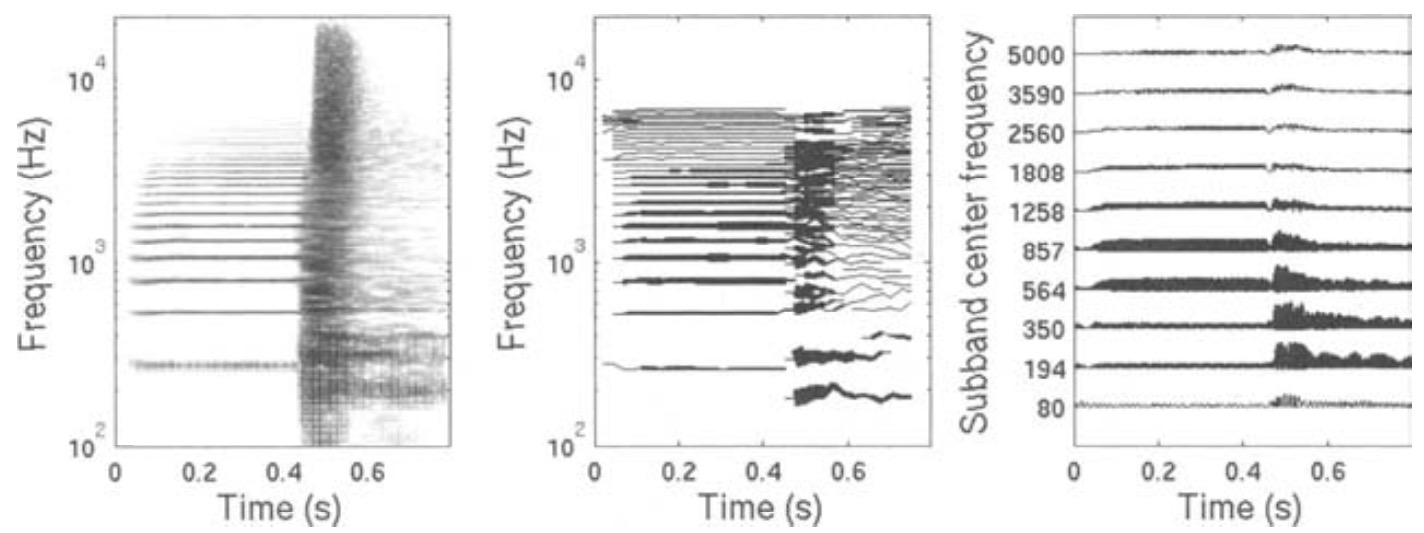
\includegraphics[scale=0.3]{images/mid_level_representation.jpg}\\
  \caption{Grafy przedstawiają 3 różne reprezentacje danych na średnim poziomie tego samego dźwięku trąbki grającej dźwięk C4. Lewy wykres przedstawia spectrogram na logarytmicznej skali częstotliwości. Środkowy wykres przedstawia reprezentację ścieżek sinusoidalnych, przy czym szerokość lini oznacza amplitudę poszczególnych sinusoid. Prawy wykres przedstawia prosty model słuchowy. Wykres z \cite[14]{Transcription:Zatorre:AuditoryCortex}}
  \label{fig:mid_level_representation}
  \end{center}
\end{figure}



\subsection{Transformata Fouriera}\label{sec:TF}
Pliki dźwiękowe zawierają informacje, które reprezentują siłę ciśnienia akustycznego w domenie czasu. Jest to jedna z reprezentacji, która może być analizowana w celu zbadania konkretnych cech sygnału, lecz jest ona bezpośrednim efektem nagrania muzyki i możliwości jej bezpośredniego odtworzenia. Dokładna analiza relacji sygnału muzycznego, jego reprezentacja jak i jego zrozumienie odbywa się po przeniesieniu na płaszczyznę częstotliwości. W muzyce zachodniej, F0 w zapisie nutowym definiuje się jako wysokość dźwięku w rozumieniu częstotliwości, co zostało po omówione w sekcji \ref{subsec:pitch}.

Aby z sygnału akustycznego w domenie czasu uzyskać dane w domenie częstotliwości powszechnie używane jest narzędzie matematyczne o nazwie \textbf{transformata Fouriera}. Funkcja ta jest uniwersalna i powszechnie stosowana w analizie sygnałów, w tej pracy jednak skupię się się na opisaniu sposobów wykorzystywania jej do celów analizy sygnałów akustycznych. Transformata ta opiera się na założeniu, że każdą okresową krzywą można zapisać w postaci sumy składowych sinusoidalnych o różnych częstotliwościach. Funkcja ta przekształca sygnału z dziedziny czasu na dziedzinę częstotliwości, co daje zarys tego jak rozłożona jest częstotliwość poszczególnych częstotliwości w analizowanych danych. Transformata zadana jest wzorem:

\begin{equation} \label{eq:fourier-base}
CFT_x(f) = X(f) = \int_{-\infty}^{\infty}\textit{f}(t)e^ {-j2\pi ft}\mathrm{d}t
\end{equation}
Gdzie F(f) nazywane jest transformatą Fouriera f(t) lub widmem częstotliwościowym. Wynik transformaty jest listą liczb zespolonych, dzięki czemu można ją odwrócić przy pomocy odwrotnej transformaty Fouriera (IFT, ang. \textit{Inverse Fourier Transformation}) opisanej wzorem:

\begin{equation} \label{eq:inverse:fourier-base}
ICFT_x(f) = \int_{-\infty}^{\infty}\textit{F}(t)e^ {j2\pi ft}\mathrm{d}t = x(t)
\end{equation}
\cite{TransformacjaFourieraWroc}\cite{TransformacjaFourieraAgh}\cite[22-25]{Transcription:Anssi:SignalProcessingMethods}.

Do analizy całego spektrum utworu muzycznego, pojedyńcza transformata Fouriera może nie być wystarczająca ze względu na długość i zróżnicowanie utworu względem czasu. Reprezentacja czasu-częstotliwości pozwala na przedstawienie sygnału w postaci zespolonej w domenie czasu i częstotliwości (ang. time–frequency representation, TFR). W celu uzyskania takiej reprezentacji przy pomocy FT z zastosowaniem okna czasowego, co jest szerzej opisane w sekcji \ref{sec:STFT}. Okna te pełnią rolę prostego TFR, spektrogramu jak i reprezentację czasową czy reprezentację opóźnienia czasowego \cite[21-22]{Transcription:Anssi:SignalProcessingMethods}.

\subsubsection{Dyskretna transformata Fouriera} \label{sec:DFT}
Jednym z założeń transformacji Fouriera jest aby f(t)\ref{eq:fourier-base} była funkcją ciągłą na przedziale od minus nieskończoności do nieskończoności, co przekłada się na transformatę w tym właśnie zbiorze. Z praktycznego punktu widzenia nieskończone granice sumy są niemożliwe do zrealizowania w analizie sygnału akustycznego, ponieważ przetwarzane są tylko skończone długości krzywych, co powoduje, że granice są zawsze skończone. W celach analitycznych na sygnałach, zwłaszcza w kontekście transkrypcji muzycznej, dane brane pod uwagę są brane z ograniczonego przedziału czasowego. Potrzebne do tego celu będzie podzielenie analizowanych danych na krótkie próbki \cite{TransformacjaFourieraWroc}\cite{TransformacjaFourieraelektronikab2b}.

\textbf{Dyskretna transformata Fouriera (DFT)} jest narzędziem matematycznym analogicznym do podstawowej transformaty Fouriera, lecz przeznaczonym do analizowania sygnału dyskretnego $x(n)$ o okresie $N$, opisanego następującym wzorem:
\begin{equation} \label{eq:DFT-periodicy}
  x(n) = x(n + mN)
\end{equation}
Pozwala ona na analizę pojedyńczego okresu zadanego sygnału. Własność ta jest szczególnie przydatna przy komputerowej analizie sygnałów, w tym fonicznych. Jest to transformacja zawsze odwracalna. 

DFT zakłada wyznaczenie iloczynu sygnału i okna prostokątnego (o którym więcej znaleźć można w sekcji \ref{sec:STFT}), które to jest wycinkiem krzywej sygnału podlegającym analizie. W związku z cyklicznością zakładanego sygnału (\ref{eq:DFT-periodicy}) przyjmuje się, że analizowany sygnał jest okresowy z okresem równym $N$, co implikuje obliczenie dokładnie N składowych harmonicznych analizowanych danych (N różnych częstotliwości). Dyskretny czas, częstotliwość i skończona liczba próbek zadanego sygnału sprowadza omawianą transformacje do funkcji w pełni dyskretnej. Wynik dyskretyzacji TF jest następujące równanie:
\begin{equation} \label{eq:DFT}
  DFT_x(k) = X(k) = \sum_{n = 0}^{N-1} x(n)e^{-j{2 \pi}kn},  k = 0, 1, 2,..., N-1
\end{equation}
DFT, tak samo jak FT jest odwracalna, co można opisać wzorem:
\begin{equation} \label{eq:IDFT}
  IDFT_x(n) = \sum_{k = 0}^{N-1} X(k)e^{j2\pi kn} = x(n), n = 0, 1, 2,..., N-1
\end{equation}
Wynikiem transformacji będzie N liczb odpowiadających kolejno amplitudzie i fazie sinusoid od $- \frac{1}{2} \Delta $ do $\frac{1}{2} \Delta $, gdzie $\Delta$ jest częstotliwością próbkowania, w rozdzielczości $\frac{1}{N} \Delta$. Częstotliwości są ustalone przez częstotliwość próbkowania oraz liczbę próbek w oknie. Jak opisuje Tomasz Zieliński w \cite[198 - 200, 204-206]{CyfrowePrzetwarzanieSygnalowOdTeoriiDoZastosowan}, DFT stanowi pewną aproksymację $N$-elementowego wektora próbek analizowanego sygnału za pomocą $N$ ortogonalnych wektorów bazowych $N$-elementowych, z wyjątkiem sytuacji, kiedy w sygnale występuje składowa sinusoidalna, która nie jest częścią zbioru wektorów bazowych, bo w takim wypadku zostanie ona przedstawiona jako suma większej liczby sygnałów "bazowych", co oznacza, że jej widmo ulegnie rozmyciu.

\subsubsection{Szybka transformacja Fouriera} \label{sec:FFT}
DFT omawiana w sekcji \ref{sec:DFT} jest wystarczająca do wykonania wszelkich analitycznych przekształceń. Problem jednak pojawia się w praktyce, i jest nim efektywność algorytmu. W swojej czystej formie transformata Fouriera $F_n$ wymaga zliczenia wszystkich wartości od $h_0$ do $h_{N-1}$ dla każdej z częstotliwości $n$, co oznacza, że złożoność obliczeniowa dla N danych wynosi $O(N^2)$, co jest zbyt dużym obciążeniem nawet dla najlepszych pod względem mocy obliczeniowej współczesnych komputerów do analizy dużego zbioru danych. Istnieje wiele metod optymalizacji numerycznych równań \ref{eq:DFT} i \ref{eq:IDFT} zmniejszających złożoność obliczeniową do co najwyżej $O(N log_2 N)$. Algorytmy te nazywają się \textbf{szybkimi transformacjami Fouriera (FFT, z ang. Fast Fourier Transform)} i to z nich korzysta się powszechnie przy cyfrowej analizie sygnałów \cite{Transcription:Tukey:FFT}.

Istnieje wiele algorytmów zaliczających się do grupy algorytmów FFT. Popularnym algorytmem jest algorytm \textbf{Cooleya-Tukeya} w formie \textbf{Radix-2} (FFT o podstawie 2). Korzysta on z metodologii \textit{dziel i zwyciężaj}, dzieląc próbkę danych wielkości $N$ na dwie oddzielne przeplatane grupy wielkości $N_1$ i $N_2$ $(N_1 + N_2 = N)$ o indeksach parzystych (0, 2, 4, ...) i nieparzystych (1, 3, 5, ...) wykonując DFT na każdym ze zbiorów, a następnie odtwarza kompletne widmo sygnału z otrzymanych wyników częściowych. W uproszczeniu algorytm wygląda następująco:
\begin{enumerate}
  \item{Zmiana kolejności próbek. Próbki dzielone są rekurencyjnie na próbki o indeksach parzystych i nieparzystych tworząc przeplatane ciągi, aż do uzyskania zbiorów dwuelementowych.}
  \item{Na każdym z uzyskanych zbiorów wykonuje się DFT, czyli łącznie $\frac{N}{2}$ dwupunktowych DFT.}
  \item{Proces składania widm powtażamy tak, że dwuprążkowe widma składane są w czteroprążkowe, czteroprążkowe w ośmioprążkowe itd., do momentu, w którym odtworzone zostanie widmo N-prążkowe, czyli kompletne widmo sygnału.}
\end{enumerate}
Co daje łączną ilość etapów operacji równą $\log_2 N$. \cite[241-252]{CyfrowePrzetwarzanieSygnalowOdTeoriiDoZastosowan}

\subsubsection{Krótkoczasowa transformata Fouriera}\label{sec:STFT}
Do tej pory przeanalizowane zostało działanie i podstawowe odmiany algorytmu transformacji Fouriera, jednak aby można było wykorzystać to narzędzie przy analizie utworów muzycznych niezbędne jest wprowadzenie reprezentacji czasu-częstotliwości TFR. \textbf{Krótkoczasowa transformacja Fouriera (STFT)} jest przeznaczona do operowania na małym oknie czasowym analizowanego sygnału. Pojedyńcze okno o indeksie $i_0$ z funkcją okna $w$ opisane jest wzorem:
\begin{equation} \label{eq:windowing}
  s_{i_0}^w = x(t)w(t_0 - t)
\end{equation}
Do funkcji okna standardowo używa się funkcji Gaussiana, Hamminga, Hanninga lub kwadratowej (choć tą ostatnią używa się tylko w wyjątkowych sytuacjach). Dokłądniejszy ich opis znajduje się pod koniec tego rozdziału. Podczas analizy i syntezy wykorzystywane jest pojedyńcze okno. Definicja STFT w dziedzinie czasu i częstotliwości można zbudować na podstawie równania \ref{eq:windowing} i FFT jako FT kolejnych okien:
\begin{equation} \label{eq:STFT1}
  STFT^{W}_{x}(t,f) = CFT_{s \frac{w}{t}}(f) = \int_{-\infty}^{+\infty} x(\tau)w(t - \tau)e^{-j2\pi f\tau}  \,\mathrm{d}\tau.
\end{equation}

W równaniu \ref{eq:STFT1} funkcja $\gamma(x)$ oznacza czasowe okno obserwacji, zaś $\Gamma(f)$ jest jej widmem Fouriera. Rozmiar okna dobierany jest zgodnie z zapotrzebowaniem, które sprowadza się do charakterystyki analizowanych danych. Dla przykładu, podczas detekcji mowy okno powinno być jak najmniejsze, ponieważ dynamika tonacji przy każdym słowie jest bardzo wysoka, i w celu odpowiedniego przeanalizowania wypowiedzi zsamplowane fragmenty, które poddawane są STFT powinny być jak najmniejsze, aby analiza była wrażliwa na nawet najdrobniejsze zmiany w tonie w celu właściwego wykrycia formantów \cite[804–816]{Transcription:Klapuri:MultipleFundamentalFrequencyEstimation}\cite[56-57, 256-258]{Transcription:Hess:PitchDetectionOfSpeechSignals}.

Równanie \ref{eq:STFT1} nosi nazwę metody "przesuwającego się okna" MWM (\textit{ang. Moving Window Method}) w dziedzinie czasowej lub częstotliwościowej. STFT wykonywane w dziedzinie czasowej sprowadza się do wykonywania przekształcenia Fouriera na kolejnych fragmentach wyciętego sygnału poprzez przesuwanie okna $\gamma(x)$. W dziedzinie częstotliwościowej algorytm STFT jest równoznaczny z:
\begin{enumerate}
  \item \label{sec:STFT:item1}odwrotnym przekształceniem Fouriera fragmentu widma sygnału poprzez przesunięcie w częstotliwości widmo okna $\Gamma(v -f)$,
  \item przesunięciem w częstotliwości sygnału czasowego otrzymanego z punktu \ref{sec:STFT:item1} do częstotliwości zerowej poprzez wymnożenie go z $exp(-j2 \pi ft)$.
\end{enumerate}
\cite[455-458]{CyfrowePrzetwarzanieSygnalowOdTeoriiDoZastosowan}

Bardzo małe okna czasowe dają większą dokładność w domenie czasowej niż częstotliwościowej. Dla algorytmów wykrywających tonacje muzyki precyzja w częstotliwości jest dużo bardziej istotna niż precyzja w czasie. Technika, która pozytywnie wpływa na dokładność w obu tych płaszczyznach, zakłada nakładanie na siebie okna, przesuwając je mniej niż jego właściwą szerokość. W zależności od tego jak mocno okno się na siebie nakłada proporcjonalnie rośnie koszt obliczeniowy tego algorytmu (np. długość okna równa 2048 sampli, a przesunięcie równe 1024 sample spowoduje nakładanie się na siebie okien przy jednoczesnym podwojeniu ilości koniecznych obliczeń). Dokładniejszy opis tego zjawiska wraz z szczegółowym opisem istotnych cech, jakie wpływają na trafność wyboru długości i algorytmu okna można znaleźć w \cite{WindowChoiceStrategiesSTFT}.


\begin{figure}[t]
  \begin{center}
    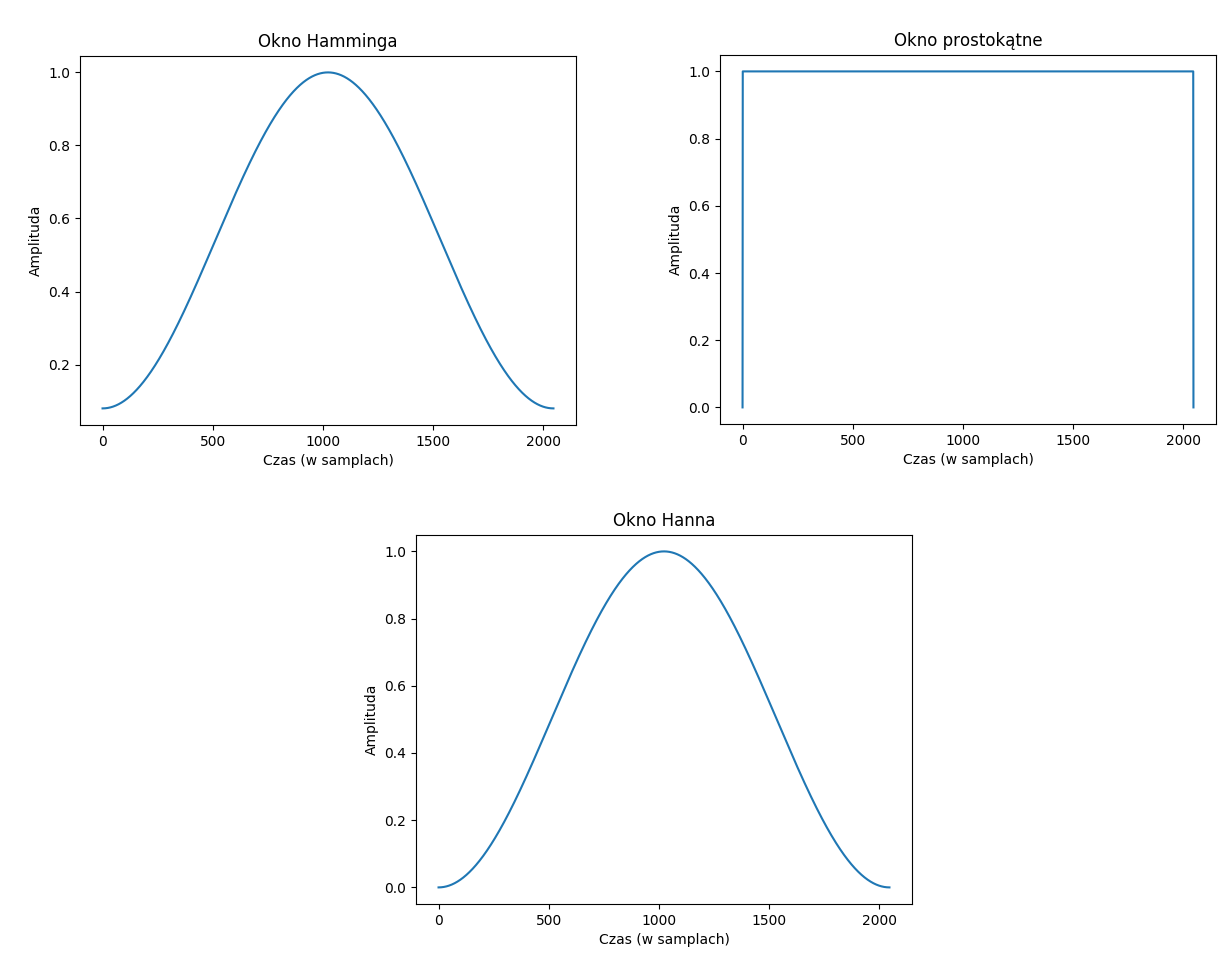
\includegraphics[scale=1.4]{images/WindowFunctions.png}
    \caption{Przykład funkcji okna czasowego dla ramki audio zawierającej 2048 sampli}
    \label{fig:WindowFunctions}
  \end{center}
\end{figure}


W momencie, gdy w algorytmie okno nakłada się na siebie, pewna porcja danych jest duplikowana. Ilość redundantnych danych jest proporcjonalna do szerokości nakładania się na siebie okien. Aby zminimalizować ten negatywny efekt, na okno nakładana jest funkcja dalej zwana funkcją okna. W ogólności, funkcja okna wydobywa odpowiednio przemnożone wartości wewnątrz jej zakresu (w oknie) i stałą wartość (zazwyczaj jest to zero) wszędzie poza obrębem zakresu okna. Dla okien czasowych można stosować wiele różnych funkcji matematycznych. W tabeli ~\ref{tab:definicjeOkien} przedstawione są funkcje $w(t)$, które często wykorzystywane są jako okna czasowe w analizie sygnału akustycznego, wraz z ich analitycznymi wzorami widm $W(\omega)$. Graficzna reprezentację okna prostokątnego, Hanna oraz Hamminga można zobaczyć na rysunku \ref{fig:WindowFunctions}\cite[103, 106]{CyfrowePrzetwarzanieSygnalowOdTeoriiDoZastosowan}\cite{Transcription:Kunieda:Aclos}.

\begin{table}[t]
  \begin{center}
    \begin{tabular}{ |c|c|c| } 
    \hline
    Nazwa funkcji & $w(t)$ & $W(\omega)$\\
    \hline
    Prostokątna & $p_T (t) = \left\{
      \begin{array}{ll}
        1 \text{ dla } |t| <= T\\
        0 \text{ dla } |t| > T\\
      \end{array}
    \right.  $ & $2\frac{\sin \omega T}{\omega}$\\
    \hline
    Trójkątne (Bartletta) & $q_T = \left\{
      \begin{array}{ll}
        1-|t|/T \text{ dla } |t| <= T\\
        0 \text{ dla } |t| > T\\
      \end{array}
    \right. $ & $T[\frac{\sin(\omega T / 2)}{\omega T/2}]^2$\\
    \hline
    Hanninga (Hanna) & $[0,5 + 0,5 \cos(\pi t / T)]p_T (t)$ & 
    $\frac{\pi^2 \sin(\omega T))}{\omega(\pi^2 - T^2 \omega^2)}$\\
    \hline
    Hamminga & $[0,54 + 0,46\cos(\pi t/T)]p_T (t)$ & 
    $\frac{(1,08\pi^2 - 0,16T^2\omega^2)}{\omega(\pi^2 - T^2 \omega^2))}\sin(\omega T)$\\
    \hline
    \end{tabular}
  \end{center}
  \caption{Definicje funkcji okien czasowych $w(t)$ i analityczne wzory ich widm $W(\omega)$}
  \label{tab:definicjeOkien}
\end{table}

\subsubsection{Przetwarzanie transformacji Fouriera}\label{sec:przetwarzanieFFT}
Wynikiem FFT jest wektor liczb zespolonych, którego długość jest równa długości danych (wielkości okna + długość wypełnienia zerami). Urojona część wyniku transformaty jest niezbędna do odwrócenia procesu transformacji, lecz nie jest niezbędna w procesie analizy. Większość algorytmów używających FFT przetwarza i skaluje wynik, aby pozbyć się niepotrzebnych informacji a istotne cechy uwypuklić. Powszechnie używaną techniką podczas analizy sygnałów jest operowanie na logarytmie amplitudy spektrum \cite[501-507]{Transcription:Talkin:RAPT}. Polega to na zastosowaniu normy Gaussa na każdej z wartości spektrum, co w rezultacie zniweluje część urojoną komponentu, a następnie zastosowanie na wyniku logarytmu naturalnego. Logarytm użyty jest do normalizacji i wyrównania danych przy zachowaniu relatywnych wartości. Wzór na logarytm amplitudy spektrum można przedstawić następująco:
\begin{equation}\label{eq:logPowSpec}
S_k^w(t,f) = ln||STFT_k^w(t,f)||
\end{equation}
gdzie $STFT_k$ jest $k$-tym komponentem spektrogramu. Częstą techniką jest również użycia potęgowania zamiast logarytmu, co zostało dokłądniej opisane w sekcji \ref{sec:f0:tfr}.
\todo[inline]{Wykres STFT vs log(||STFT||)}

Przy analizie częstotliwości składowych widmowych sygnału na uwadzę należy mieć twierdzenie Nyquista, zwane także jako twierdzenie Kotielnikowa - Shannona lub \textbf{twierdzeniem o próbkowaniu}. Mówi ono o istnieniu częstotliwości Nyquista, która opisana jest wzorem:
\begin{equation} \label{eq:NyquistFq}
  f_Nyquist = \frac{1}{2}v
\end{equation}
gdzie $v$ jest częstotliwością próbkowania. Częstotliwość ta jest maksymalną częstotliwością, jaką można wydobyć z sygnału o zadanej częstotliwości próbkowania. Odwracając proces, wzór \ref{eq:NyquistFq} mówi o tym, że częstotliwość próbkowania $v = \frac{1}{\delta t}$ musi być dobrana tak, aby była dwa razy większa od maksymalnej częstotliwości występującej w sygnale.

\begin{figure}[t]
  \begin{center}
    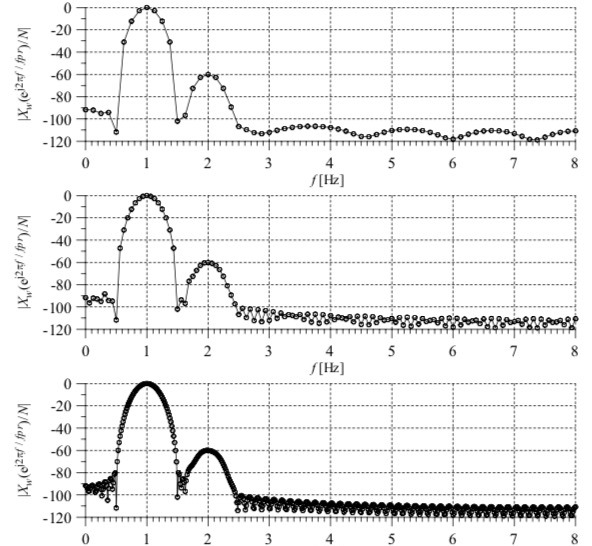
\includegraphics[scale=0.7]{images/ZeroPadding.jpg}
    \caption{Przykład analizy częstotliwościowej z wykorzystaniem STFT. Każdy z wykresów przedstawia to samo okno po uzupełnieniu na końcu zerami do długości $N_FFT$ = 128, 256, 1024 (kolejno od góry). Wykres z \cite[224]{CyfrowePrzetwarzanieSygnalowOdTeoriiDoZastosowan}}
    \label{fig:ZeroPadding}
  \end{center}
\end{figure}

Przy modelowaniu systemu transkrypcji często trzeba podjąć trudną decyzję, czy zwiększyć złożoność obliczeniową i osiągnąć lepszą aproksymację widma podczas FFT poprzez zwiększenie częstotliwości próbkowania lub zastosowanie interpolacji, czy zmniejszyć dokładność, ale otrzymać mniejszą złożoność obliczeniową. Istnieje jednak metoda, która prowadzi do kompromisu tych dwóch podejść. Polega ona na uzupełnieniu na końcu zerami analizowanego, fragmentu sygnału tuż po nałożeniu funkcji okna. Po tak wykonanej konkatenacji danych można zastosować STFT. Podejście to daje w wyniku gęściejsze próbkowanie widma przy mniejszych nakładach obliczeniowych. Tak zwiększoną rozdzielczość widma można zaobserwować na rysunku \ref{fig:ZeroPadding} \cite[221-224]{CyfrowePrzetwarzanieSygnalowOdTeoriiDoZastosowan}.

\clearpage

\subsection{Estymacja składowej fundamentalnej F0}\label{sec:f0}
Ten rozdział skupia się na opisaniu metod estymacji składowej fundamentalnej w sygnale akustycznym. Jest to jeden z kroków wymaganych do pełnej transkrypcji utworu muzycznego, a przez wielu badających ten teren nauki uważany za najważniejszy  \cite[2-4]{Transcription:Klapuri:ChallengesAndFuture}. Wysokość dźwięku jest niezwykle istotną informacją z punktu widzenia muzyka, a sposób zagrania determinowany jest właśnie przez F0. Nawiązując do informacji opisanych w rozdziale \ref{sec:JakDzialaMuzyka} aby poprawnie wykryć F0 należy mieć na uwadzę bardzo dużo czynników. 

Dalsze rozważania będą przebiegać z założeniem, że przetwarzane sygnały są z podzbioru muzyki o standardach kompozycji zachodniej, lecz bez wyszczególnionego gatunku muzycznego. Nie będziemy również skupiali się na wykryciu tak zwanych dźwięków o niezależnej wysokości, do których zaliczają się elementy perkusyjne. Ważnym założeniem, które jest stosowane w tym rozdziale, jest analiza jedynie sygnałów monofonicznych. W odróżnieniu do krzywych reprezentujących muzykę polifoniczną, w analizowanych utworach będzie grany tylko jeden dźwięk na pojedyńczym instrumencie, bez równoległych dźwięków. Algorytmy analizujące muzykę wielotonową są opisane w rozdziale \ref{sec:MultiPitch}. Jest to bardzo duże ułatwienie, ponieważ konkurujące sygnały dźwiękowe nakładają się na siebie, zmuszając algorytm analizujący do rozróżnienia i odseparowania ich przed faktyczną analizą F0. 

\subsubsection{Funkcja Autokorelacji}\label{sec:f0:ac}
Domena czasu jest najbardziej naturalną postacią sygnału dźwiękowego, ponieważ w takiej właśnie postaci jest odbierane przez ludzkie ucho - jako ciśnienie akustyczne zmienne w czasie. Wiele z pierwszych badań jakie prowadzono w kontekście transkrypcji sygnału fonicznego wykorzystywało tą postać sygnału, między innymi w \cite{Transcription:Gold:ComputerProgramForPitchExtraction}. Algorytm ten polegał na znajdywaniu wzorców w krzywej sygnału. Regularności które powtarzały się okresowo co $T$ były analizowane jako kandydaci do bycia F0. Jak analiza czystego binarnego sygnału i wyliczenia na nim nie są częstą praktyką, tak podejście do znajdywania wzorców i regularności jest obecna w wielu nowoczesnych algorytmach. Najbardziej dosłowne odwzorowanie tej idei można znaleźć w metodologiach opartych na korelacji w celu znalezienia wysokości dźwięku.

\textbf{Autokorelacja} jest narzędziem matematycznym stosowanym w przetwarzaniu sygnałów. Służy ono do analizy serii wartości. Ta statystyczna miara jest korelacją pomiędzy kolejnymi wartościami tej samej zmiennej. Funkcja ta ma za zadanie wykrycie regularności w analizowanych danych \cite[32-33]{CyfrowePrzetwarzanieSygnalowOdTeoriiDoZastosowan}. Proces autokorelacji polega na badaniu korelacji wejściowych danych z tymi samymi danymi, ale przesuniętymi o tak zwane przesunięcie (ang. \textit{lag}). Siła korelacji o odpowiednim przesunięciu może świadczyć o powtarzającym się wzorze w sygnale z częstotliwością przesunięcia.

W pracy naukowej \cite{Transcription:Lawrence:AutocorrelationForPitchDetection} Lawrence używa funkcji autokorelacji do wykrycia częstotliwości fundamentalnych w zadanym sygnale monofonicznym. Zakłada on, że badany sygnał jest quasi-periodyczny, co oznacza, że sygnał posiada cechy pojawiające się w prawie równych odstępach, lecz nie koniecznie dokładnie periodyczny. Sygnał w pełni periodyczny jest przedmiotem analizy czysto teoretycznej, ponieważ sygnał akustyczny musiałby pozostać bez zmian w amplitudzie i częstotliwości przez cały swój okres, podczas gdy sygnał quasi-periodyczny zakłada zmiany w strukturze sygnału względem czasu. Funkcja autokorelacji na takim sygnale byłaby funkcją długości okresu opisującą zgodność przesuniętego o ten okres sygnału z sygnałem bazowym. 

Wzór na ogólną postać funkcji autokorelacji od długości okresu $h(t)$ jako:

\begin{equation}\label{eq:AC}
  R(k) = \lim_{N \to \infty} \frac{1}{2N + 1} \sum_{n=-N}^{N} h(n)h(n + k)
\end{equation}
gdzie $k$ jest opóźnieniem, $n$ reprezentuje moment w czasie a N reprezentuje długość badanej funkcji. Jak można zaobserwować w \ref{eq:AC} założeniem jest, że sygnał bazowy jest nieskończenie długi (tak samo jak przy TF opisanej w sekcji \ref{sec:TF}). Do rozważań w kontekście analizy sygnału fonicznego będziemy używać wariancji krótkoczasowej tego wzoru, operującej na oknach danych (analogicznie do STFT opisanej w sekcji \ref{sec:STFT}) opisanej w \cite{Transcription:Talkin:RAPT} jako:

\begin{equation}\label{eq:STAC}
  R(i,k) = \sum_{j=m}^{m + N - k - 1} h_jh_{j+k}, m = iz
\end{equation}
gdzie $i$ jest indeksem badanego okna, $z$ jest odstępem pomiędzy oknami audio (ilość sampli), a N jest długością okna. Zgodnie z twierdzeniem Nyquista opisanym w sekcji \ref{sec:STFT} długość okna powinna być co najmniej dwa razy większa niż największe oczekiwane opóźnienie jakie może wystąpić w analizowanym sygnale akustycznym Implementacja estymacji F0 przy pomocy autokorelacji przy pomocy wzoru \ref{eq:STAC} została opisana dokładniej w sekcji \ref{sec:impl:alg:ac}.

Z jednego okna danych w wyniku brane jest to przesunięcie, które ma największy współczynnik korelacji. Aby z tego przesunięcia uzyskać częstotliwość, należy podzielić częstotliwość samplowania przez to przesunięcie, ponieważ domena czasu w dyskretnym sygnale na jakiej operuje autokorelacja jest tak naprawdę domeną ilości sampli.
\begin{equation}\label{eq:AC:hz}
  fq = \Delta/lag
\end{equation}

\begin{figure}[t]
  \begin{subfigure}{.5\textwidth}
    \centering
    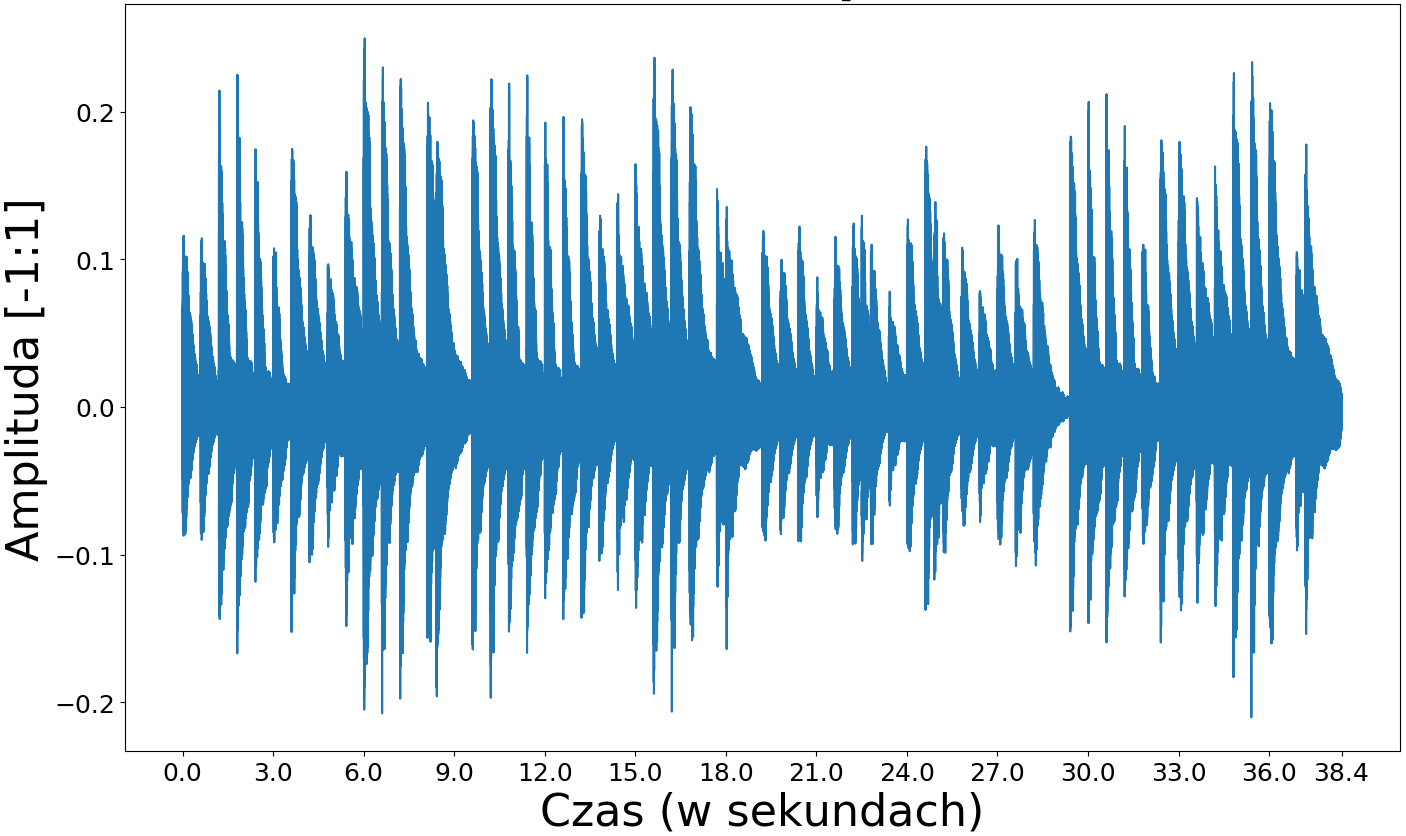
\includegraphics[width=1.\linewidth]{images/AC/fala_cropped.png}
    \caption{Fala dźwiękowa}
    \label{fig:ACResults:wave}
  \end{subfigure}%
  \begin{subfigure}{.5\textwidth}
    \centering
    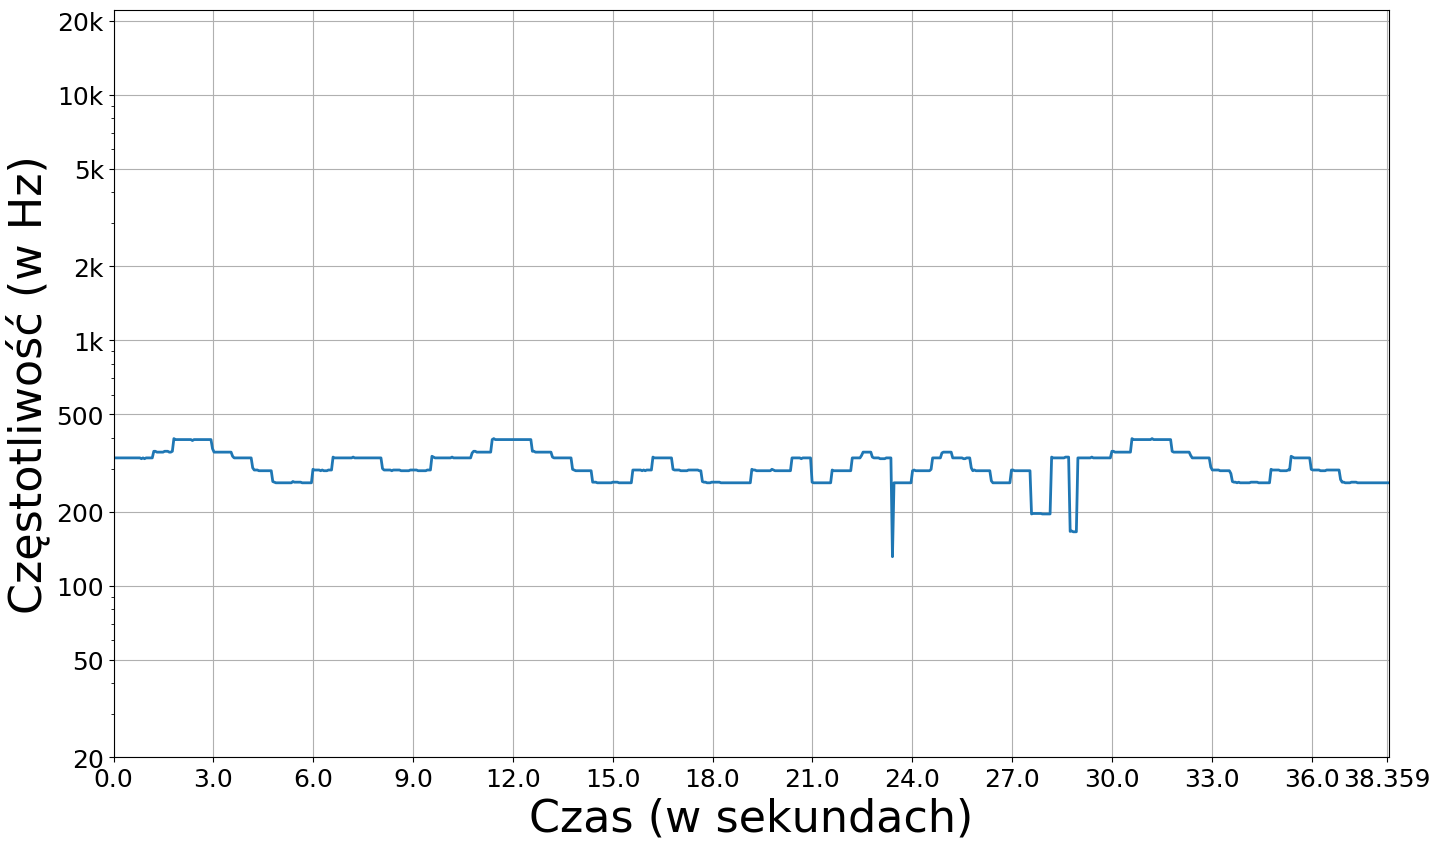
\includegraphics[width=1.\linewidth]{images/AC/f0Thick_cropped.png}
    \caption{Estymacja F0}
    \label{fig:ACResults:f0}
  \end{subfigure}
  \newline
  \begin{subfigure}{1\textwidth}
    \centering
    % include third image
    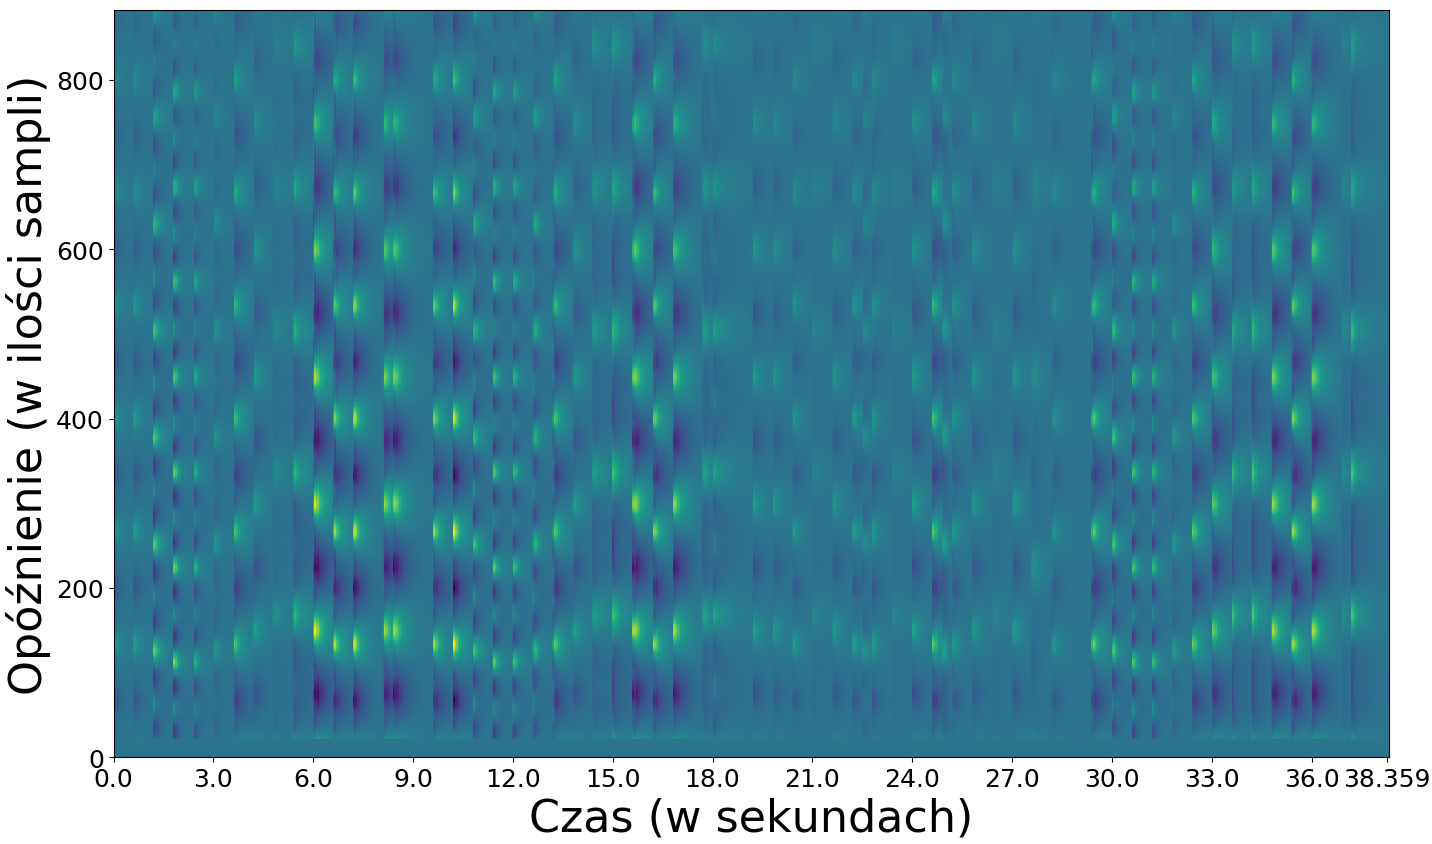
\includegraphics[width=.6\linewidth]{images/AC/korelogram_cropped.png}  
    \caption{Korelogram}
    \label{fig:ACResults:corr}
  \end{subfigure}
  \caption{Wynik autokorelacji na ,,Odzie do radości'' IX symfonii Beethovena zagranej monofonicznie na pianinie. Użyto okno Hanna o długości 2048 sampli z odstępami długości 2048 sampli. Wybór F0 polegał na wybraniu największego współczynnika korelacji w oknie. Wykresy wygenerowane przy pomocy implementacji opisanej w sekcji \ref{sec:impl:alg:ac}.}
  \label{fig:ACResults}
\end{figure}

Podstawowym założeniem algorytmów wykrywania F0 z wykorzystaniem autokorelacji (tak samo jak znormalizowanej korelacji krzyżowej, która stara się zminimalizować defekty funkcji autokorelacji. Dokładny jej opis można znaleźć w \cite{Transcription:Talkin:RAPT}) jest to, że analizowany sygnał jest monofoniczny. Jest to spowodowane tym, że periodyczność jaką cechuje się pojedyńcza krzywa quasi-periodyczna jest modulowana, albo nawet całkowicie neutralizowana po nałożeniu na nią innej krzywej. Załóżmy, że został nagrany sygnał z dwoma nutami o różnych wysokościach granymi równolegle w tym samym czasie. Okresami, w którym te sygnały w izolacji byłyby powtarzalne to $T_1$ i $T_2$. Po nałożeniu się na siebie, wynikowy sygnał nie byłby periodyczny w żadnym z tych interwałów, chyba że jeden byłby wielokrotnością drugiego Jest to opisane dokładniej w sekcji \ref{sec:MultiPitch:monofon}.

Wyniki estymacji F0 mają tendencje do bycia wielokrotnościami faktycznego F0 sygnału, co można zaobserwować na wykresach na wykresie \ref{fig:ACResults:f0}. Dzieje się tak, ponieważ wysoki współczynnik korelacji, jaki uzyska krzywa o periodyczności równej $T$ dla opóźnienia $T$ będzie relatywnie podobny do wyniku autokorelacji dla tego sygnału dla opóźnienia $2T$, $3T$ itd. Jest to spowodowane faktem, że wzorzec występujący co $T$ występuje w szczególności co $2T$, $3T$ itd. Można to również zaobserwować w korelogramie przedstawionym na wykresie \ref{fig:ACResults:corr}. \cite[238-250]{Transcription:Anssi:SignalProcessingMethods}

\subsubsection{Analiza TFR} \label{sec:f0:tfr}
Analiza sygnału w postaci reprezentacji średniego poziomu TFR, w przeciwieństwie do operowania na nieprzetworzonym sygnale cyfrowym, jak miało to miejsce w sekcji \ref{sec:f0:ac}, skupia się na badaniu relacji w domenie częstotliwości danego sygnału. Najpopularniejszą reprezentacja TRF jest zdefiniowana jako STFT na kolejnych fragmentach (oknach) sygnału. Docelową postacią jest zbór okien tworzących spektrogram, ale w celu jego uzyskania należy SFTF przedstawić jako wektor energii. Jednym ze sposobów w jaki można uzyskać taką postać jest to wykonanie kwadratu modułu z STFT:

\begin{equation} \label{eq:powSpec}
  SP_x^w(t,f) = |STFT_x^w(t,f)|^2
\end{equation} 
Wynik powyższego równania \ref{eq:powSpec} nazywany jest potocznie widmem mocy (z ang. \textit{power spectrum}). W celu uzyskania spektrogramu używa się również innych metod, jak na przykład logarytmu z modułu (co zostało to opisane w sekcji \ref{sec:przetwarzanieFFT}). Wybór metodyki zależny jest od tego, które cechy sygnału wejściowego są bardziej, a które mniej istotne w kontekście algorytmu analizującego. Użycie widma mocy wiąże się z uwydatnieniem już wyraźnych cech, wraz z zwiększeniem istotności szumu w sygnale.

\begin{figure}[t]
  \begin{subfigure}{.49\textwidth}
    \centering
    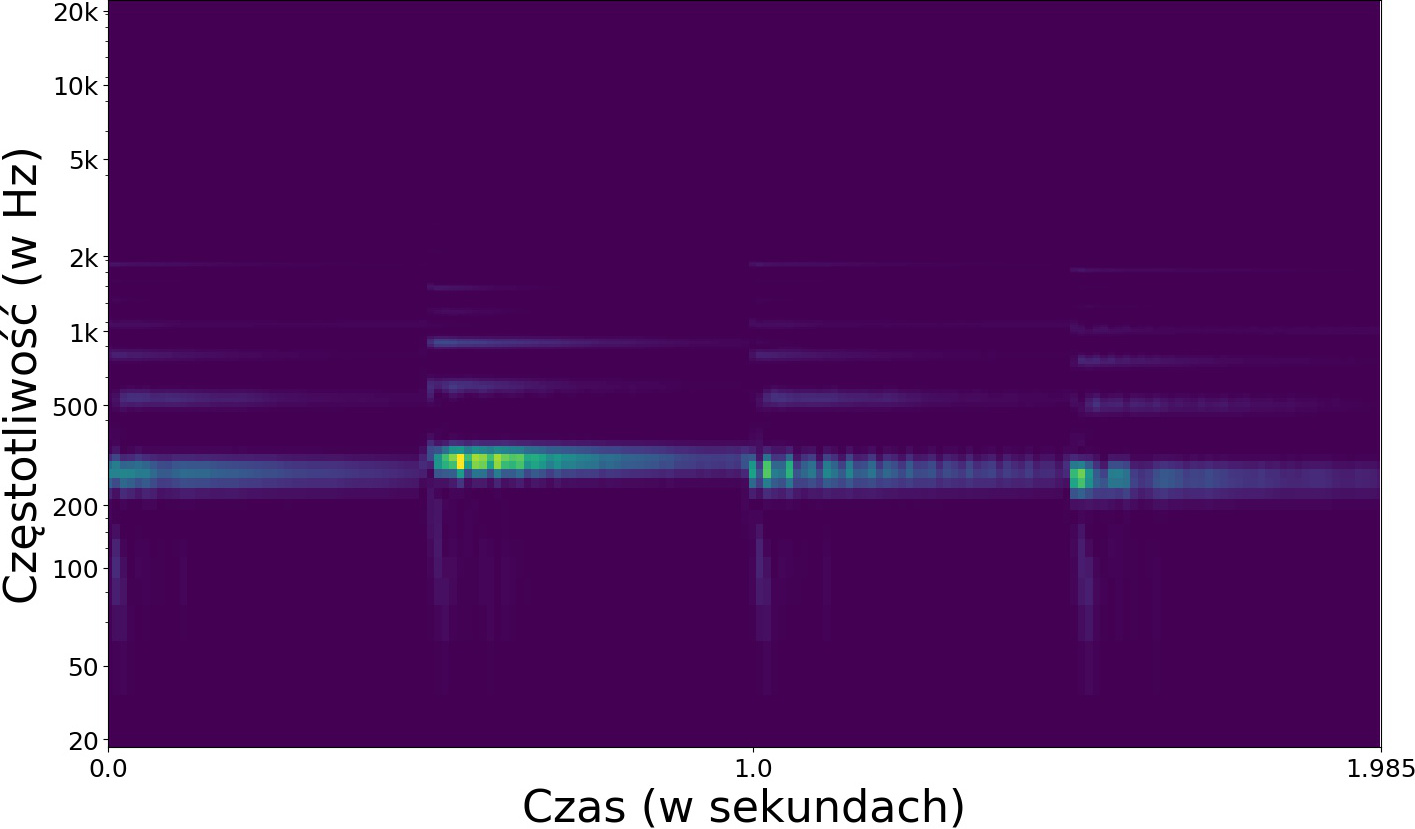
\includegraphics[width=1.\linewidth]{images/Spectrogram/spectrogram_1024_cropped.jpg}
    \caption{Spektrogram z długością okna 1024 sample}
  \end{subfigure}
  \begin{subfigure}{.5\textwidth}
    \centering
    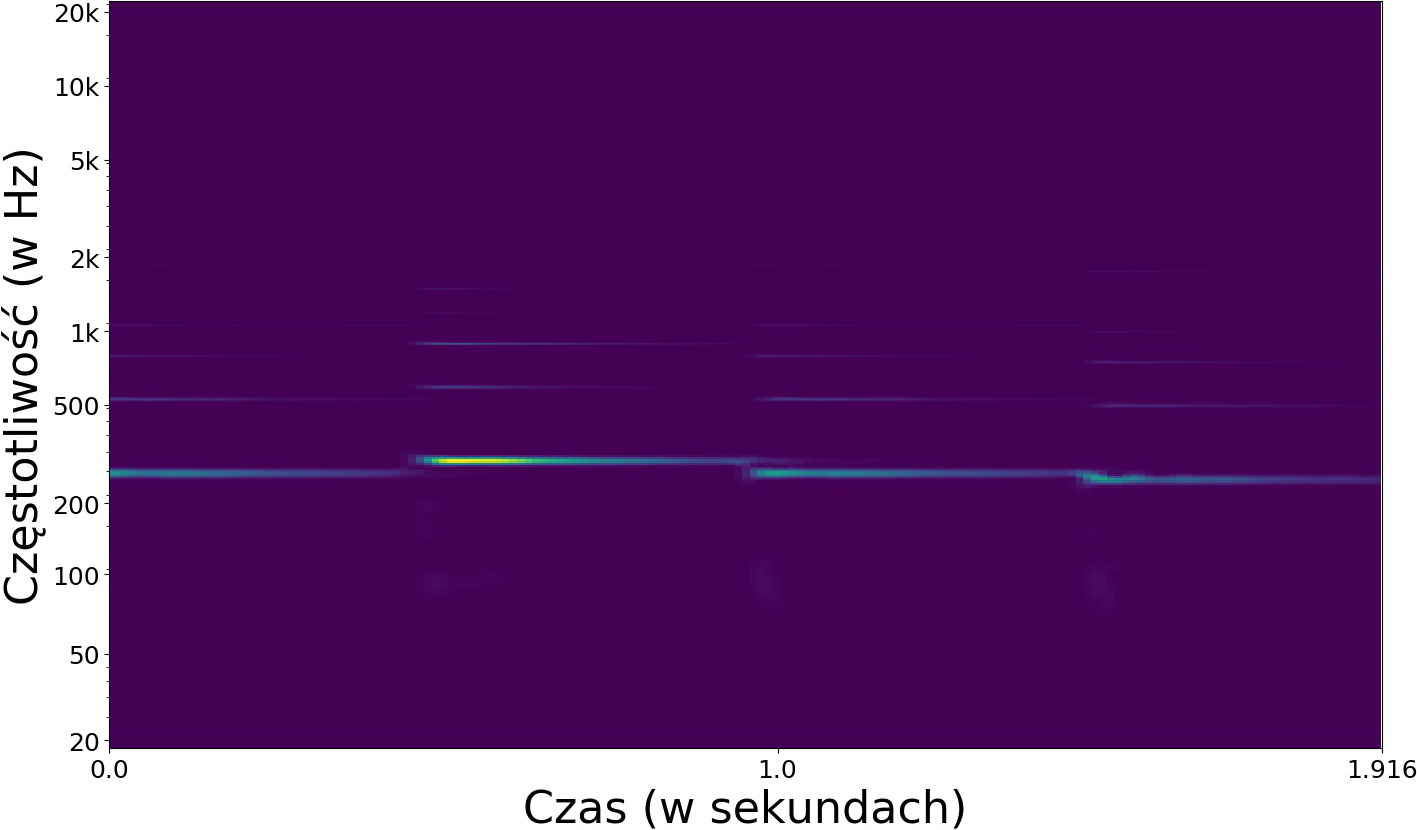
\includegraphics[width=1.\linewidth]{images/Spectrogram/spectrogram_4096_cropped.jpg}
    \caption{Spektrogram z długością okna 4096 sample}
  \end{subfigure}
  \caption{Spektrogramy sygnału sekwencji C3-D3-C3-B2 zagranej na pianinie wyliczone przy pomocy STFT z oknem Hanna długości odpowiednio 1024 i 4096 dla wykresów (a) i (b) z odstępami o długości 512 sampli.}
  \label{fig:windowSize}
\end{figure}

Zmiana funkcji okna $w$ zmieni specyfikę STFT, co przekłada się na inny wynikowy spektrogram. Długość użytego okna jest także istotną cechą spektrogramu. Zmiany w dokładności poszczególnych wartości spektrogramu przy różnych długościach okna opisane są w sekcji \ref{sec:STFT} i widoczne na ilustracji \ref{fig:windowSize}.

Podczas analizy spektrogramu, naiwnym podejściem byłoby wybranie za F0 ten pik w spektrum, który ma największą energię. Niestety jednak nie jest to zawsze prawidłowy wybór - częstotliwość fundamentalna wcale nie musi być tą, która ma najwięcej energii w sygnale akustycznym. Ze względu na charakterystyki różnych instrumentów, formanty, szum i inne zniekształcenia opisane dokłądniej w sekcji \ref{sec:barwaDzwieku} kolejne harmoniczne mogą być wzmocnione ponad F0.

\begin{figure}[t]
  \begin{center}
    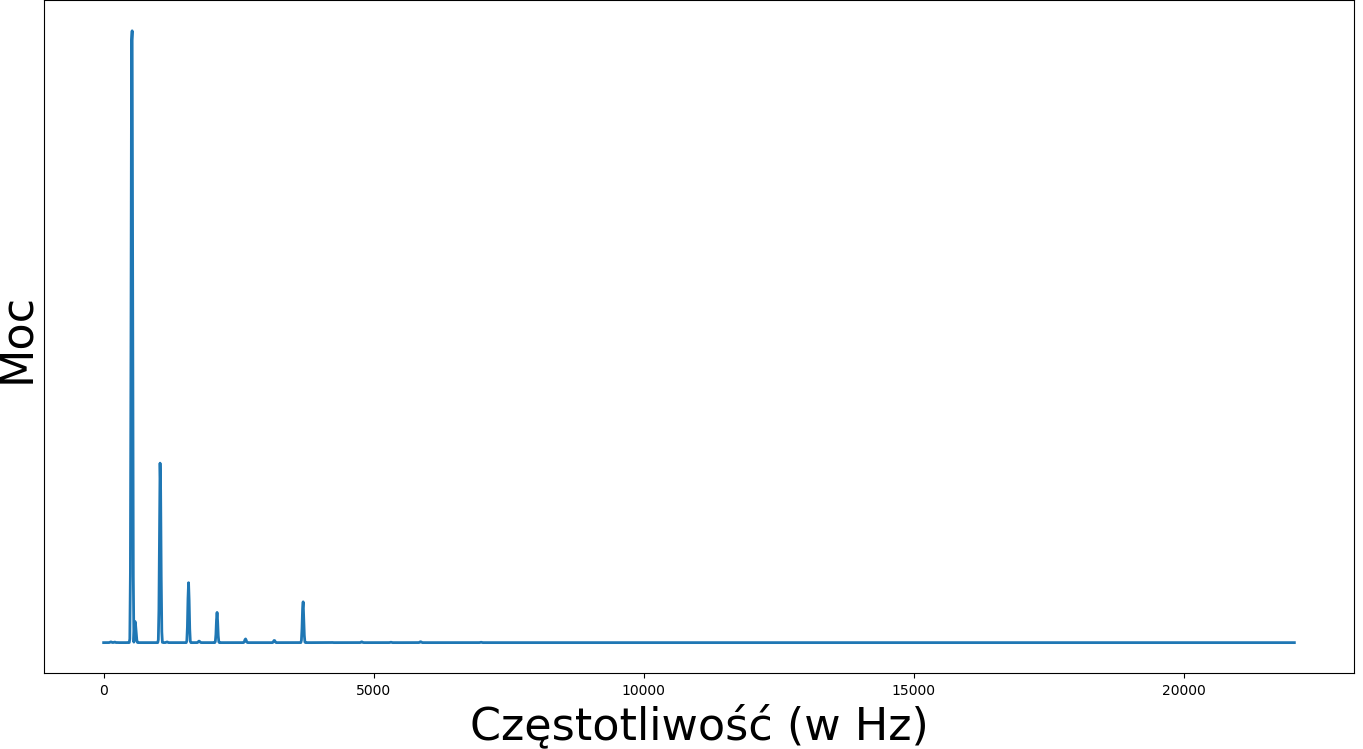
\includegraphics[scale=0.46]{images/Spectrogram/spectrum_4096_cropped.png}
    \caption{Przykład pojedyńczego komponentu spektralnego ze spektrogramu \ref{fig:windowSize} o długości okna 4096. Można zaobserwować, że na przestrzeni spektrum piki pojawiają się periodycznie w domenie częstotliwości.}
    \label{fig:spectralComponent}
  \end{center}
\end{figure}

Analiza spektrogramu w celu znalezienia F0 polega na znalezieniu sensu w rozmieszczeniu harmonicznych względem siebie. Zgodnie z regułą harmoniczności, harmoniczne sygnału mają częstotliwości będące wielokrotnościami fundamentalnej częstotliwości. Są one równomiernie rozmieszczone na przestrzeni całego spektrum, co powoduje, że pojedyńcza nuta jest sama w sobie periodyczna w domenie częstotliwości, co można zauważyć na rysunku \ref{fig:spectralComponent}. Ta charakterystyka akustycznych fal jest powszechnie używana w wykrywaniu częstotliwości fundamentalnej jako najbardziej niezawodna. Wystarczy zlokalizować pik o najmniejszej częstotliwości wraz z największą ilością pików pasujących jako kolejne harmoniczne. Używanie zasady harmoniczności, lub hybryda tych dwóch podejść poprzez ważenie energii częstotliwością jest znacznie bardziej pewną metodą wyznaczania częstotliwości fundamentalnej niż opieranie się na samym ciśnieniu akustycznym.

\subsubsection{Analiza cepstralna}\label{sec:f0:ceps}
Z racji tego, że spektrum samo w sobie jest periodyczne, można spróbować użyć metodologi wykrywającej cykliczności już na spektrum. Taki pomysł mieli już w 1963 Bogert, Healy i Tukey w \cite{Transcription:Bogert:FirstCepstrum}. Stworzyli oni narzędzie matematyczne przeznaczone dla danych zawierających echa lub pogłosy fundamentalnej częstotliwości, która nie jest znana. \textit{Cepstrum mocy} używane jest do wyznaczenia czasu początku F0, jego echa i powiązanych amplitud. Analiza na zespolonym cepstrum pozwala na powrót do pierwotnego kształtu badanego sygnału \cite{Transcription:Childers:CepstruGuide}.

Cepstrum zostało pierwotnie opisane w pracy \cite{Transcription:Bogert:FirstCepstrum}, a następnie, dwa lata później w roku 1967, zastosowane do wykrywania wysokości dźwięku w ramach \cite{Transcription:Noll:CepstrumPitchDetermination}. Jak opisuje Oppenheim i Schafer w pracy naukowej dotyczącej historii cepstrum (\cite[95-99]{Transcription:Oppenheim:HistoryOfCepstrum}) równolegle z tymi pracami, niezależnie powstawała praca doktorancka \cite{Transcription:Oppenheim:Superposition} badająca klasę nielinearnych technik przetwarzania sygnałów poprzez koncepcje homomorficznego mapowania pomiędzy grupami algebraicznymi i przestrzeniami wektorowymi. Miała ona mieć szczególne zastosowanie w metodologii cepstrum, pokrywając się wnioskami  i przyspieszając tempo jego rozwoju. Dalsze prace Oppenheima opisujące między innymi charakterystyki splotu harmonicznych, które są reminiscent do spektrum logarytmu spektrum, którym to właśnie jest cepstrum. Odkrycia te przyczyniły się do między innymi stosowania cepstrum na oknach czasowych (tak jak STFT) czy opisanie zespolonego cepstrum, które pozwala na odwrócenie tej transformacji, otwierając drogę do takich metod jak filtrowanie w domenie cepstralnej.


Oryginalnie analiza cepstralna opisana w pracy \cite{Transcription:Bogert:FirstCepstrum} została zdefiniowana jako "spektrum mocy z logarytmu spektrum mocy". Nawiązując do wzoru \ref{eq:logPowSpec}, cepstrum mocy okna o indeksie $k$ z oknem $w$ liczy się jako 
\begin{equation}\label{eq:ceps1}
  C_k^w(t, f) = |(S_k^w(t,f)|^2.
\end{equation}
Pierwotnym zastosowaniem tego narzędzia było wykrycie echa w sygnale sejsmicznym. Podejście to było bardziej odporne na barwę sygnału od wcześniej używanej funkcji autokorelacji (opisanej w sekcji \ref{sec:f0:ac}). Zastosowanie to było czysto analityczne, i nie wymagało od algorytmu możliwości przywrócenia analizowanych danych do domeny czasu. Mimo, że jednym z autorów \cite{Transcription:Bogert:FirstCepstrum} jest Tukey, który także pracował nad FFT, cepstrum zostało opublikowane na dwa lata przed algorytmem FFT \cite{Transcription:Tukey:FFT}, przez co jego potencjał nie był jeszcze odkryty. Choć w oryginalnej pracy nad cepstrum zdefiniowane były takie pojęcie jak ,,lifter'', był zainicjalizowany później z użyciem filtra splotowego \cite[1-2]{Transcription:Randall:CepstrumHistory}. 

Nazwa cepstrum bierze się z odwrócenia pierwszych liter wyrazu \textit{spectrum} (z ang. spektrum). Bogert, Healy i Tukey w pracy \cite{Transcription:Bogert:FirstCepstrum} opisali szereg terminologii związanej z cepstrum, między innymi takie jak:
\begin{table}[H]\centering
  \begin{tabular}{lll}
  \textit{rahmonics} & zamiast & \textit{harmonics} (z ang. harmoniczność) \\
  \textit{liftering} & zamiast & \textit{filtering} (z ang. filtrowanie) \\
  \textit{quefrency} & zamiast & \textit{frequency} (z ang. częstotliwość) \\
  \textit{gamnitude} & zamiast & \textit{magnitude} (z ang. wielkość)
  \end{tabular}
\end{table}
\noindent Wytłumaczeniem tej lingwistyki, w której znajome wyrazy były modyfikowane w celu uzyskania czegoś podobnego, ale mimo wszystko troche innego, było zadeklarowane następująco: "Ogólnie rzecz biorąc, działamy po stronie częstotliwości w sposób powszechnie stosowany po stronie czasu i odwrotnie"\cite{Transcription:Bogert:FirstCepstrum} \cite[1-4]{Transcription:Randall:CepstrumHistory}.

Cepstrum przedstawia piki tam, gdzie oryginalny sygnał w przestrzeni czasu\-amplitudy posiada echo. Ta nowa reprezentacja spektralnej domeny nie jest już domeną częstotliwości, ani też nie jest to domena czasu. Przez ten fakt, aby nie mieszać tych pojęć ze znanymi pojęciami Bogert nazwał domenę cepstrum jako domena \textit{quefrency}, która tak naprawdę jest domeną częstotliwości spektralnych pików oryginalnego sygnału.

W przypadku lifterowania, czyli filtrowania w domenie quefrency, przydatnym wzorem jest cepstrum sygnału ciągłego $x(t)$:
\begin{equation}\label{eq:ceps:continous}
Cep_x(\tau) \ ICFT_{log(|X|)}(\tau) = \int_{-\infty}^{\infty}  log(|X(f)|)e^{j2\pi f\tau}\,\mathrm{d}f, 
\end{equation}
gdzie  $X(f)$ oznacza TF. Zgodnie ze wzorem \ref{eq:ceps:continous} filtrowanie sygnału w domenie częstotliwości przez wynik $X(f)H(F)$ staje się, po wzięciu $log$, sumą $log[X(f)] + log[H(f)]$ gdzie $H(f)$ jest filtrem częstotliwościowym \cite[25-27]{Transcription:Anssi:SignalProcessingMethods}.

\begin{figure}[t]
  \begin{subfigure}{.49\textwidth}
    \centering
    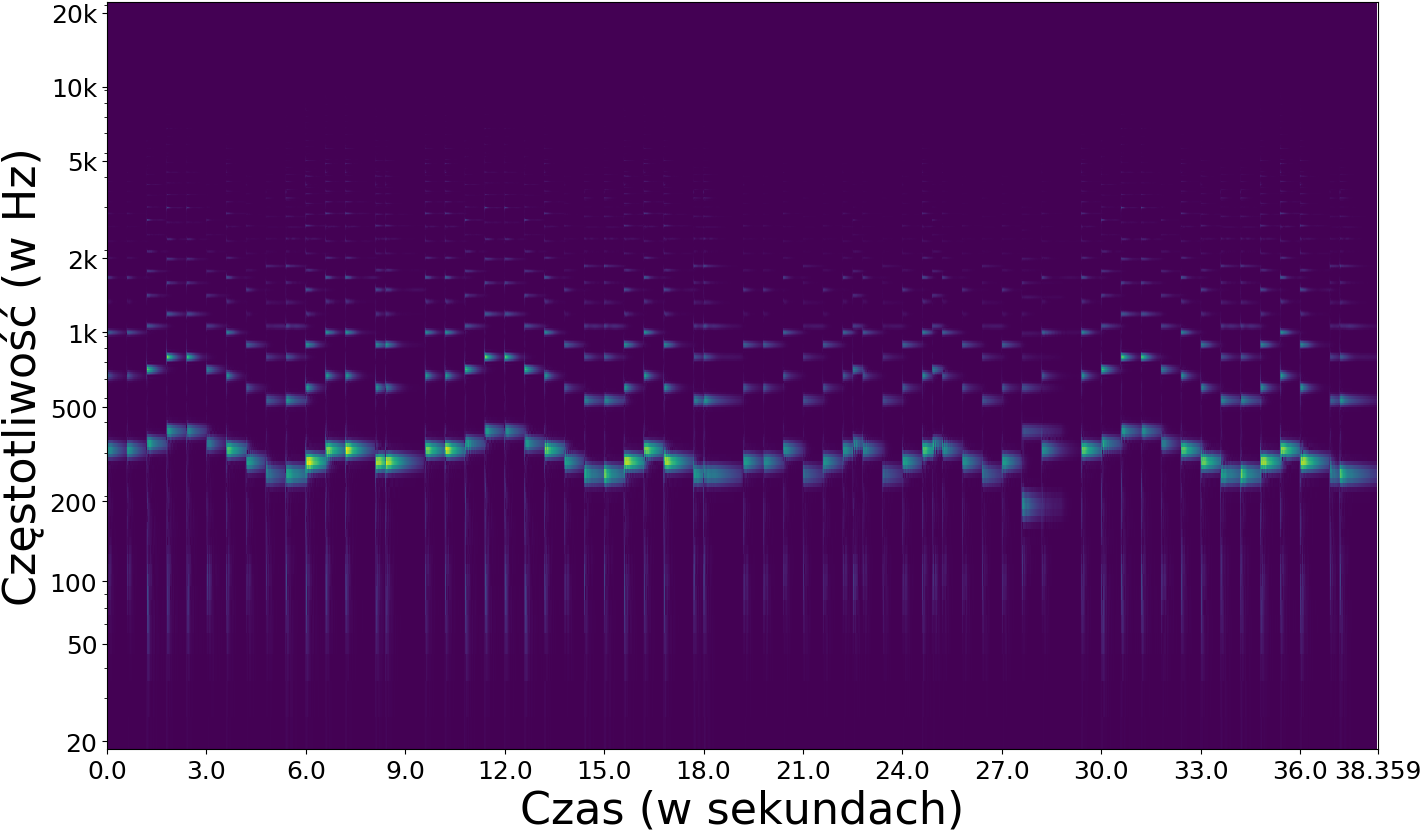
\includegraphics[width=1.\linewidth]{images/Cepstrum/spec_cropped.png}
    \caption{Spektrogram}
  \end{subfigure}
  \begin{subfigure}{.5\textwidth}
    \centering
    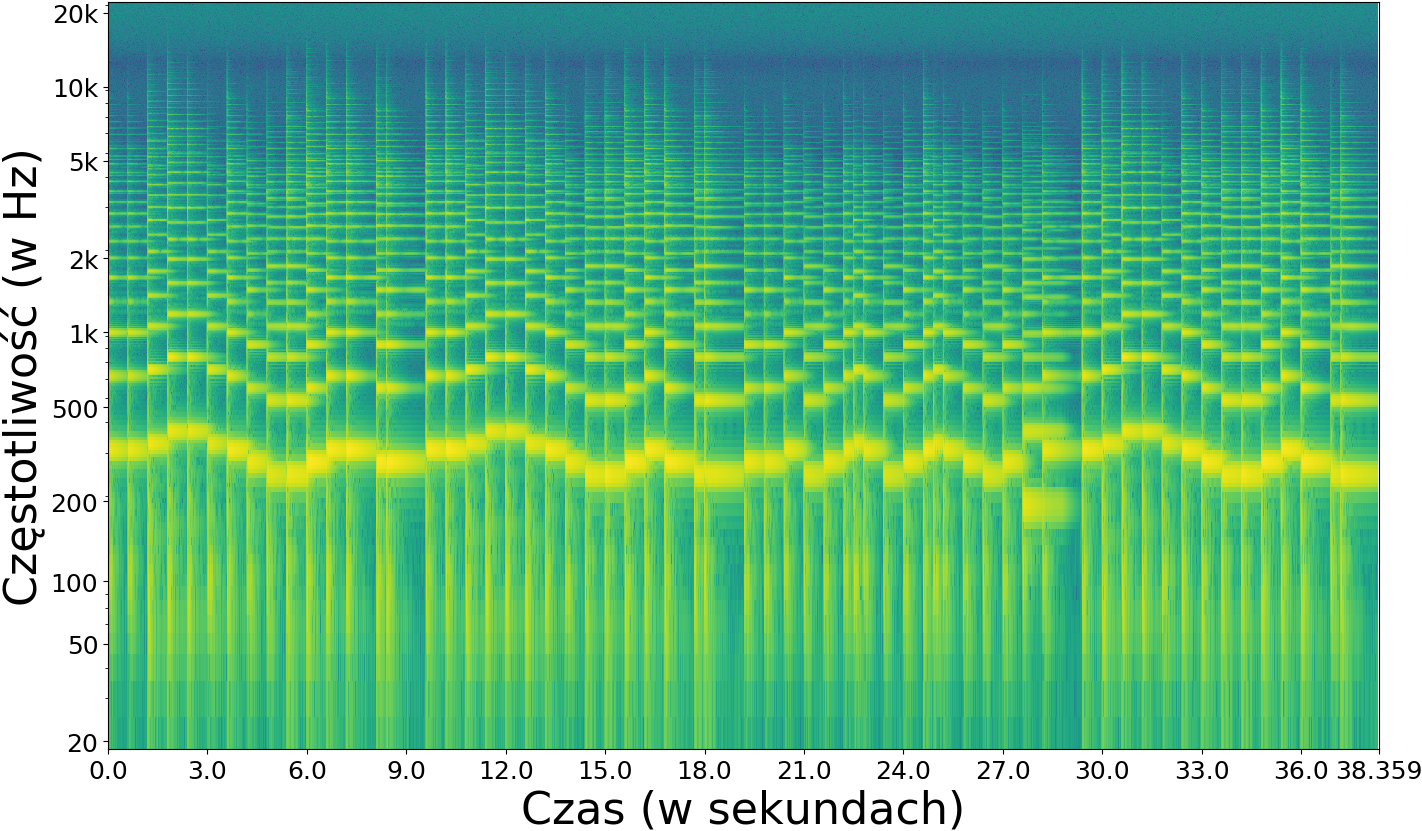
\includegraphics[width=1.\linewidth]{images/Cepstrum/log_pow_spec_cropped.png}
    \caption{Logarytm spektrogramu mocy}
  \end{subfigure}
  \newline
  \begin{subfigure}{.49\textwidth}
    \centering
    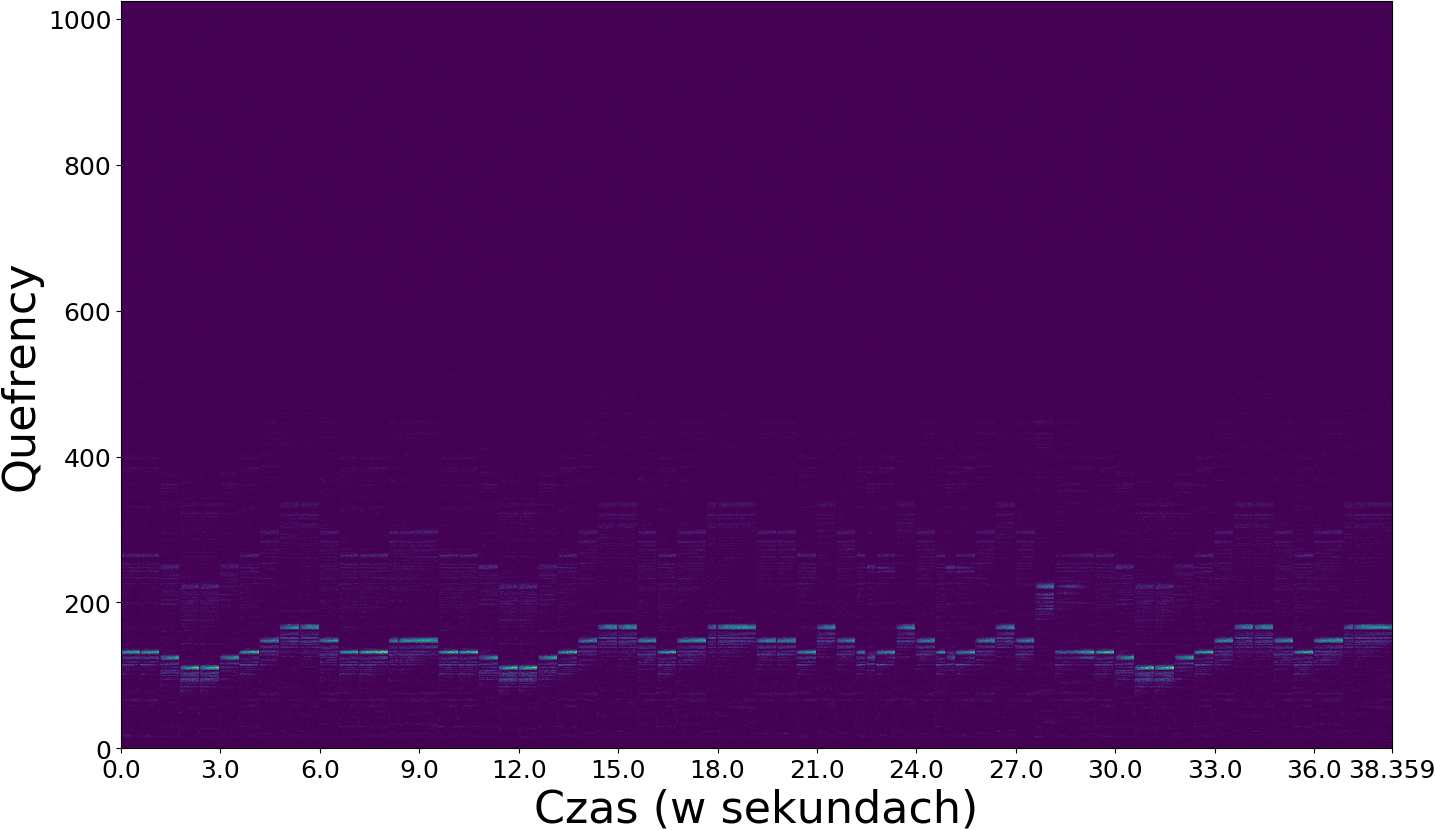
\includegraphics[width=1.\linewidth]{images/Cepstrum/cepstrogram_cropped.png}
    \caption{Cepstrogram}
  \end{subfigure}
  \begin{subfigure}{.5\textwidth}
    \centering
    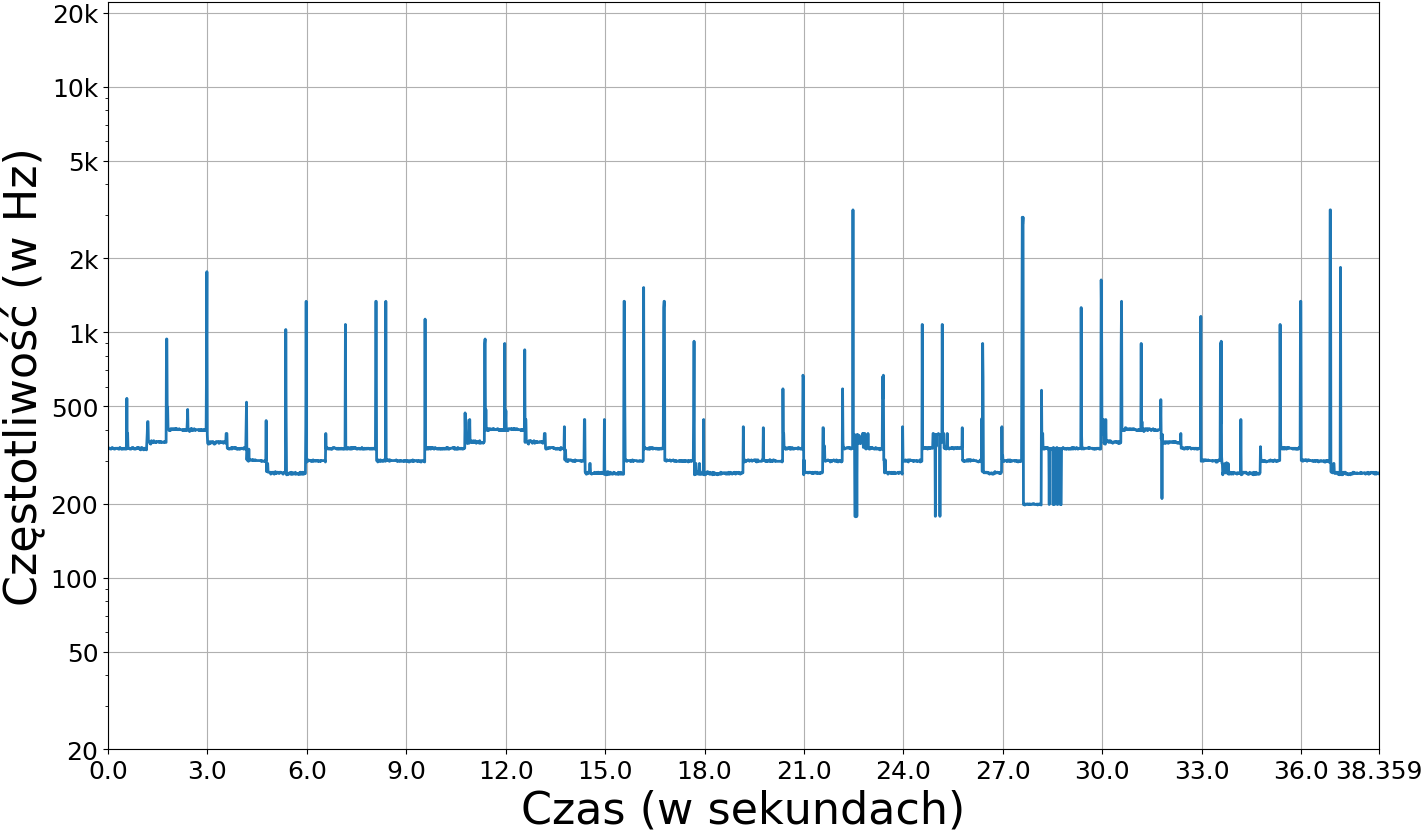
\includegraphics[width=1.\linewidth]{images/Cepstrum/estymacjaF0_cropped.png}
    \caption{Estymacja F0}
  \end{subfigure}
  \caption{Wynik cepstrum na na ,,Odzie do radości'' IX symfonii Beethovena zagranej monofonicznie na pianinie. Użyto okno Hanna o długości 2048 sampli z odstępami długości 512 sampli. Wybór F0 polegał na wybraniu największego współczynnika cepstralnego w oknie. Wykresy wygenerowane przy pomocy implementacji opisanej w sekcji \ref{sec:impl:alg:ceps}.}
  \label{fig:cepstrumF0}
\end{figure}

Postać cepstralną sygnału akustycznego można bezpośrednio wykorzystać do znalezienia częstotliwości fundamentalnej w monofonicznym sygnale. Podejście to operuje na cepstrum mocy, które opisane jest wzorem \ref{eq:ceps1}, dla kolejnych okien czasowych. Tak pozyskane cepstrum badane jest w kontekście kandydatów F0, i wybierany ten, z największym współczynnikiem. Dokładna implementacja opisana jest w sekcji \ref{sec:impl:alg:ceps}. Metoda ta jest podatna na wyznaczanie wielokrotności F0, zamiast faktycznej częstotliwości fundamentalnej, tak jak metoda autokorelacji \ref{sec:f0:ac}. Ten defekt można zaobserwować na ilustracji \ref{fig:cepstrumF0}. To podejście nie radzi sobie też z sygnałami zawierającej dużą ilość szumów, co jest przedstawione w \cite[233-235]{Transcription:Kunieda:Aclos}. Mimo tych wad, metodyka cepstrum jest powszechnie stosowana w analizie sygnałów. Jej ważnym zastosowaniem jest filtrowanie przy pomocy lifteringu, które używane jest między innymi w opisanym algorytmie ACLOS \ref{sec:f0:aclos}.

\subsubsection{ACLOS}\label{sec:f0:aclos}
Badanie cykliczności spektrum, do którego jednym z narzędzi jest cepstrum opisane w \ref{sec:f0:ceps}, można wykorzystać również narzędzia autokorelacji. Omówiona wcześniej metoda badająca cykliczność na cyfrowej fali akustycznej poprzez wyliczanie autokorelacji (\ref{sec:f0:ac}) użyta w domenie częstotliwości została opisana w 1996 roku w \cite{Transcription:Kunieda:Aclos} pod nazwą \textbf{ACLOS}. Oba te algorytmy polegają na zasadzie cykliczności fal akustycznych i harmonicznych F0, próbując wykryć dokłądny odstęp pomiędzy cyklami.

\begin{figure}[H]
  \begin{center}
    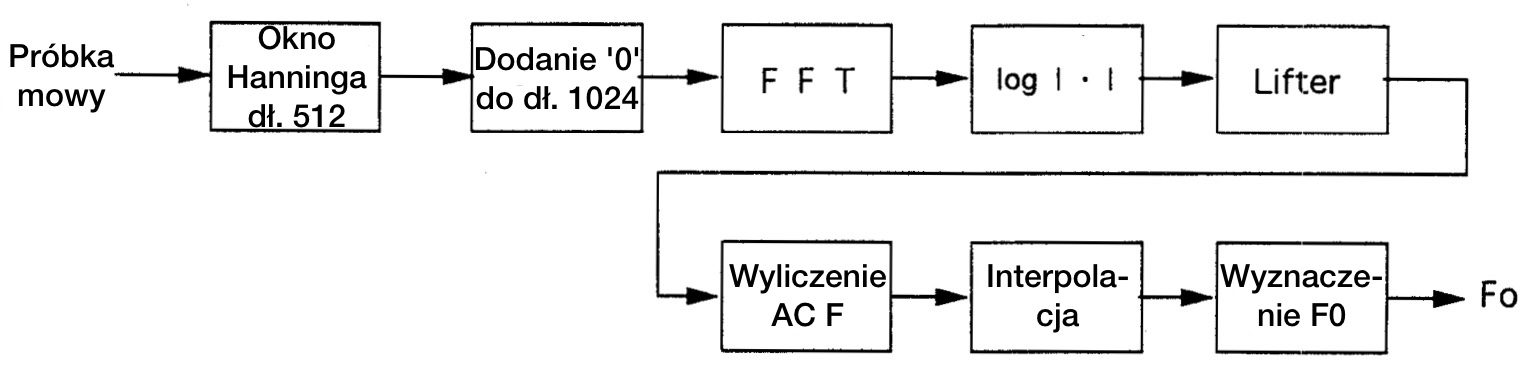
\includegraphics[scale=0.29]{images/ACLOS/ACLOS_flow.jpg}
    \caption{Schemat działania algorytmu ACLOS do wykrywania wysokości dźwięku. Schemat z \cite[233]{Transcription:Kunieda:Aclos}.}
    \label{fig:aclos:flow}
  \end{center}
\end{figure}

Nazwa algorytmu ACLOS jest skrótem od \textit{AutoCorrelation of LOg Spectrum}, co oznacza autokorelację na logarytmie widma. Motywacją do stworzenia ACLOS było odkrycie takiego algorytmu, który wykorzysta zalety cepstrum i jednocześnie będzie bardziej odporne na szumy w badanym sygnale. Dodatkowo, autorzy ACLOS przytaczają prace naukową \cite{Transcription:Lahat:SpectralAutocorrelationNoiseCorrupted}, która również wykorzystuje autokorelacje na widmie sygnału akustycznego, z ta różnicą, że nie stosuje się na nim logarytmowania, a proces autokorelacji determinowany jest procedurą decyzyjną w zależności od pików na poszczególnych pasmach sygnału, czo czyni ten algorytm dużo bardziej skomplikowany niż ACLOS.


\begin{figure}[H]
  \begin{center}
    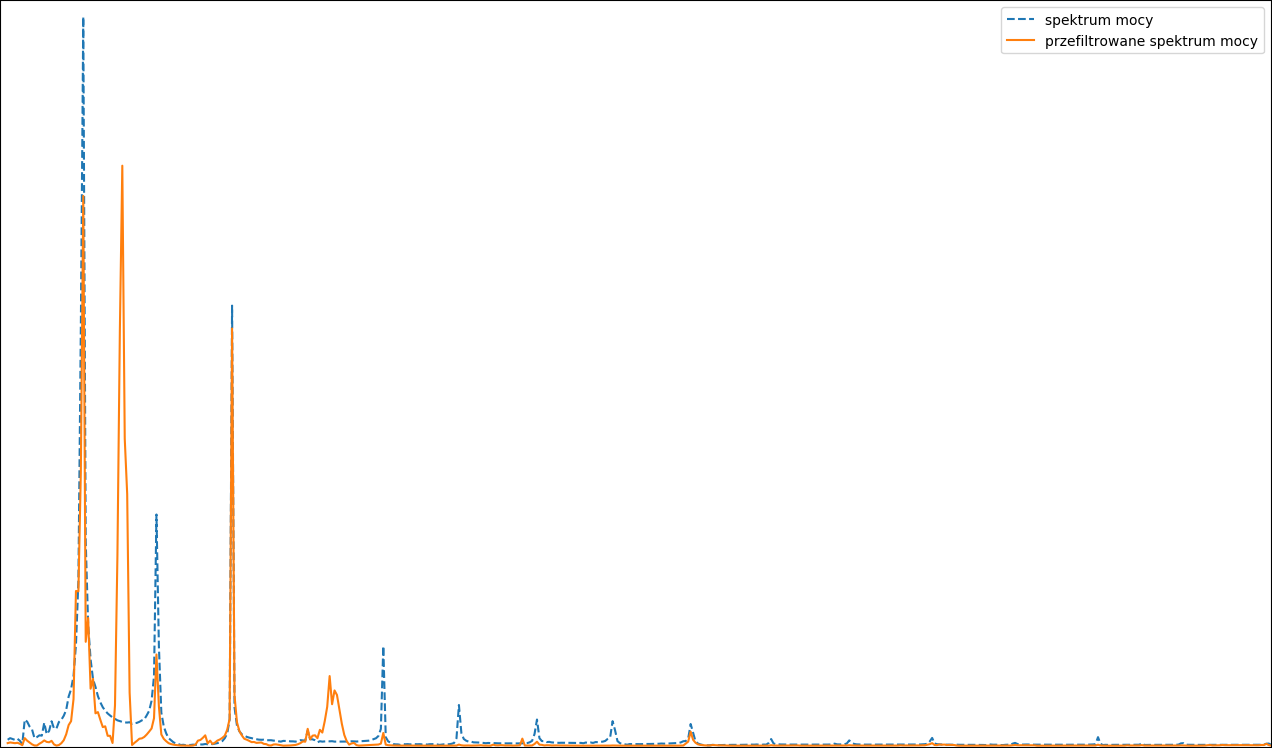
\includegraphics[scale=0.49]{images/ACLOS/data_lifter_cropped.png}
    \caption{Wykres przedstawiający spektrum na pojedyńczym oknie przed i po nałożeniu lifteringu ze współczynnikiem równym 10}
    \label{fig:aclos:lifter}
  \end{center}
\end{figure}
Schemat działania algorytmu ACLOS dla okna Hanninga o długości 512 sampli przedstawiony jest na rysunku \ref{fig:aclos:flow}. W zależności od długości okna zmieniać się będzie wynikowa częstotliwość i maksymalna częstotliwość jaką można wykryć w sygnale (zgodnie z równaniem Nyquista przedstawionym w \ref{eq:NyquistFq}). Do okna doklejana jest odpowiednia ilość zer jako margines, które mają na celu zwiększenie częstotliwości widma, co zostało opisane w sekcji \ref{sec:przetwarzanieFFT}. W oryginalnej pracy dodano 512 zer, aby wynikowe okno miało długość 1024. Na rozszerzonym o wektor zer oknie wyliczana zostaje szybka transformata fouriera, a z niej wynik przetwarzany jest do logarytmu spektrum mocy zgodnie ze wzorem \ref{eq:powSpec}. Następną operacją jaka jest wykonywana na analizowanych danych jest filtrowanie w domenie cepstrum. Liftering ma w tym przypadku na celu wyrównanie spektrum i zmniejszenie wpływu jaki ma na wynik szum. Wynik działania lifteringu można zaobserwować na wykresie na rysunku \ref{fig:aclos:lifter}. Na tak przygotowanym oknie wykonywana jest funkcja autokorelacji $R(j)$, która ma postać:
\begin{align}\label{eq:Aclos:ACf}
  R(j)& = \frac{1}{N}\sum_{i=0}^{N-1}f(i)f(i + j)&
  j = 0, 1, ..., M
\end{align}
gdzie $f(i)$ jest i-tym komponentem lini widmowej, $N$ oznacza maksymalną harmoniczną, która jest brana pod uwagę, $j$ jest częstotliwością dla której badany jest współczynnik autokorelacji a $M$ oznacza maksymalną częstotliwość, jaką może posiadać F0 w analizowanym sygnale.

\begin{figure}[ht]
  \begin{subfigure}{.49\textwidth}
    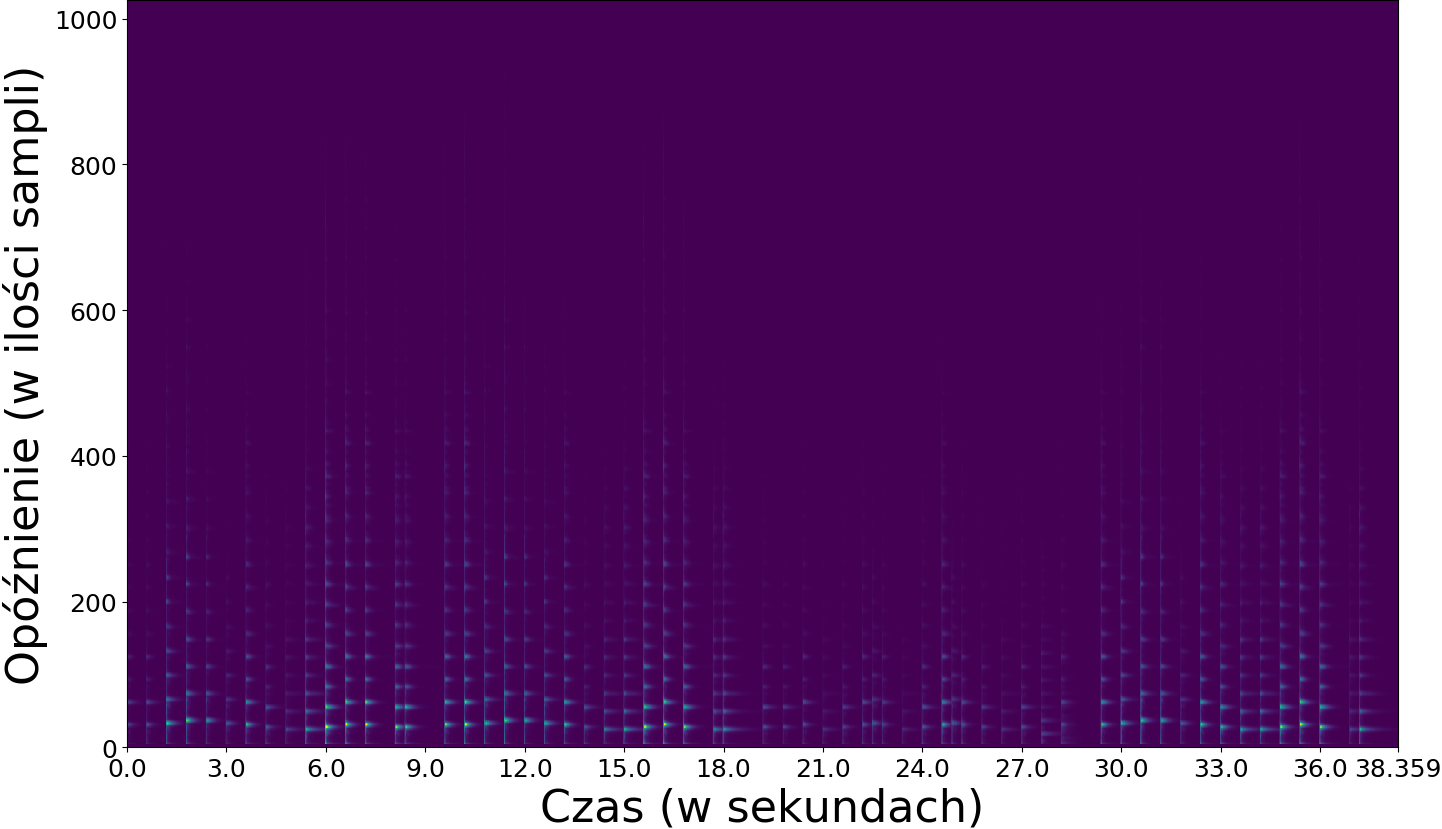
\includegraphics[width=1.\linewidth]{images/ACLOS/Korelogram_cropped.png}
    \caption{Korelogram}
  \end{subfigure}
  \begin{subfigure}{.5\textwidth}
    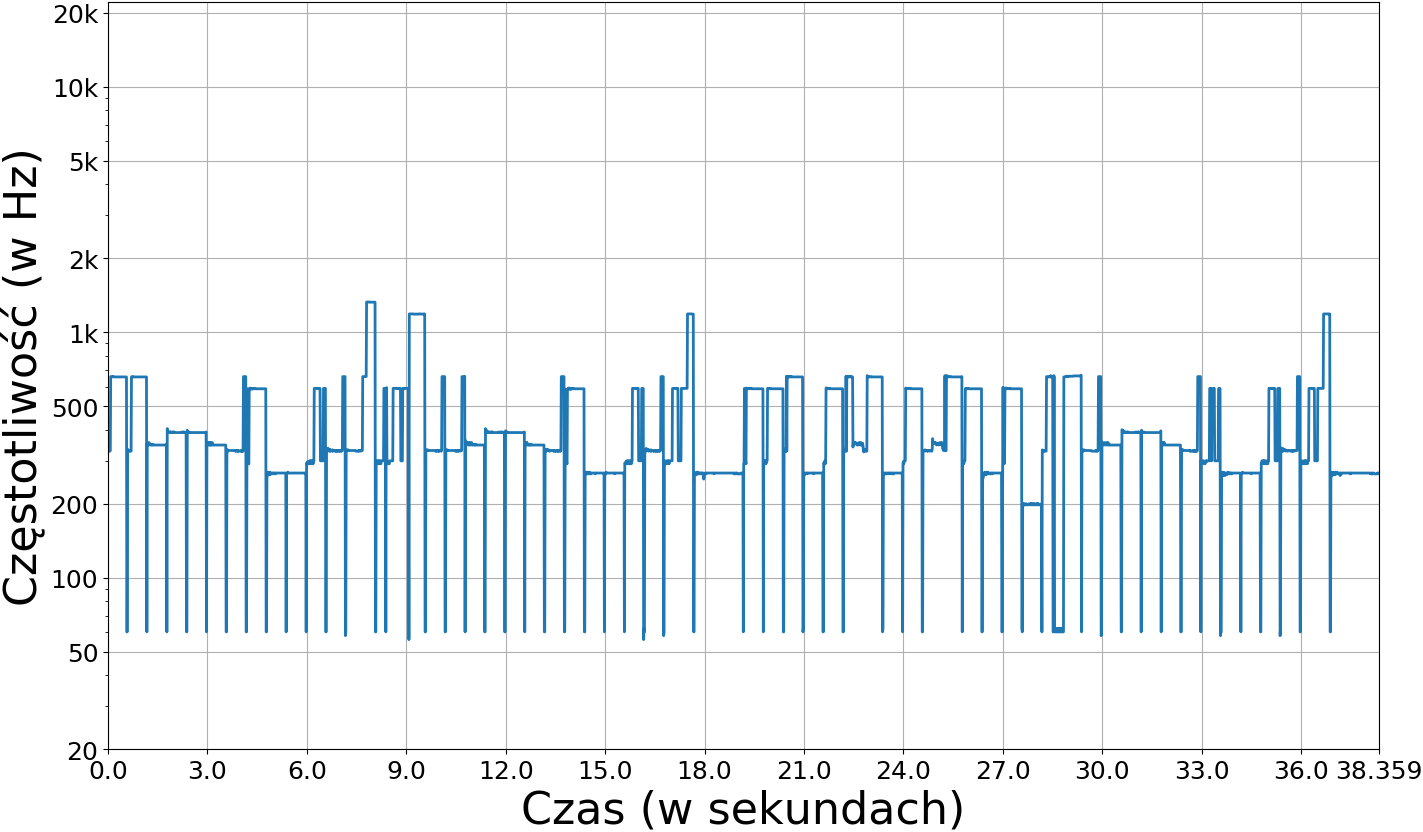
\includegraphics[width=1.\linewidth]{images/ACLOS/Estymacja_f0_cropped.png}
    \caption{Estymacja F0}
  \end{subfigure}
  \newline
  \begin{subfigure}{0.5\textwidth}
    \centering
    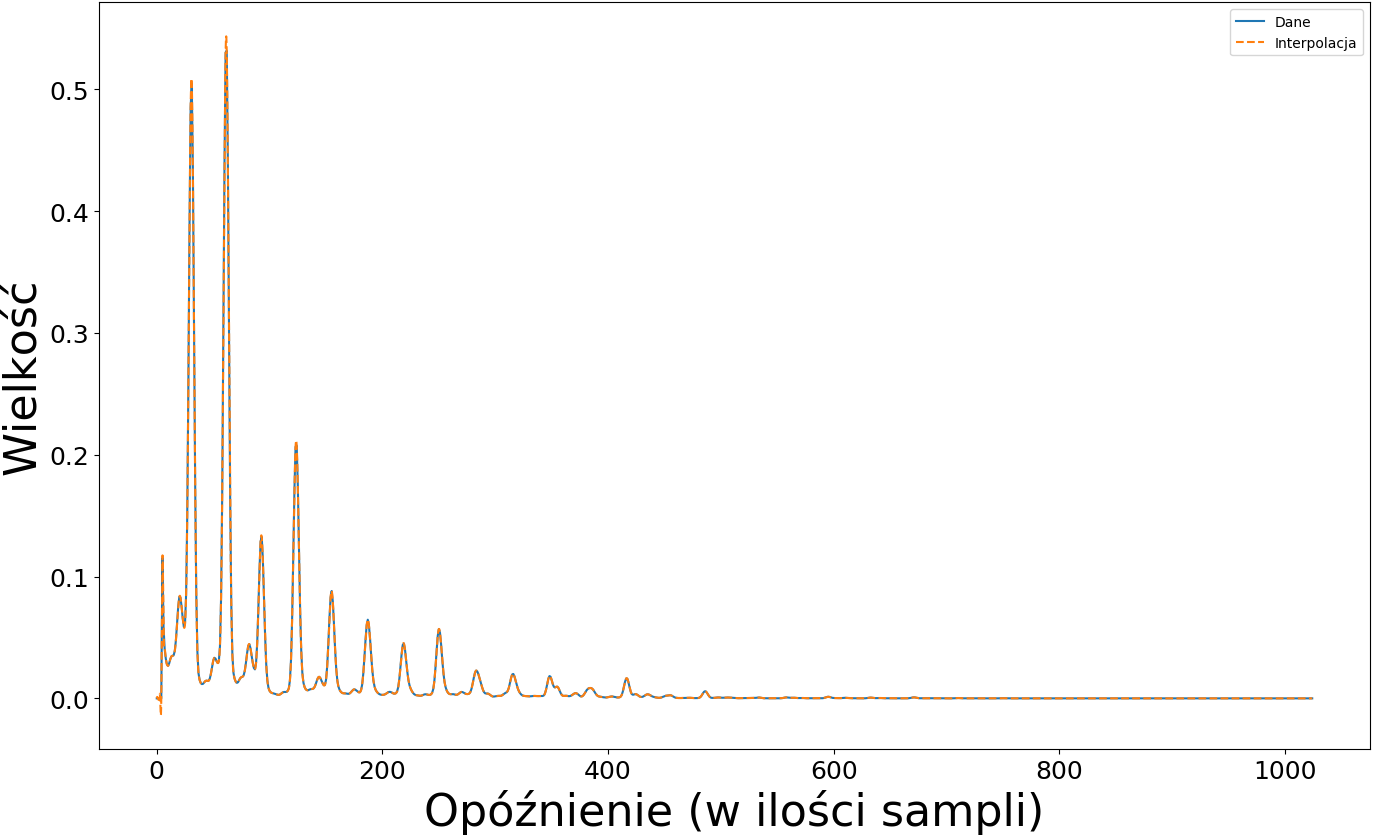
\includegraphics[width=1.\linewidth]{images/ACLOS/interpolacja_full_cropped.png}
    \caption{Okno autokorelacji i jego interpolacja}
  \end{subfigure}
  \begin{subfigure}{0.49\textwidth}
    \centering
    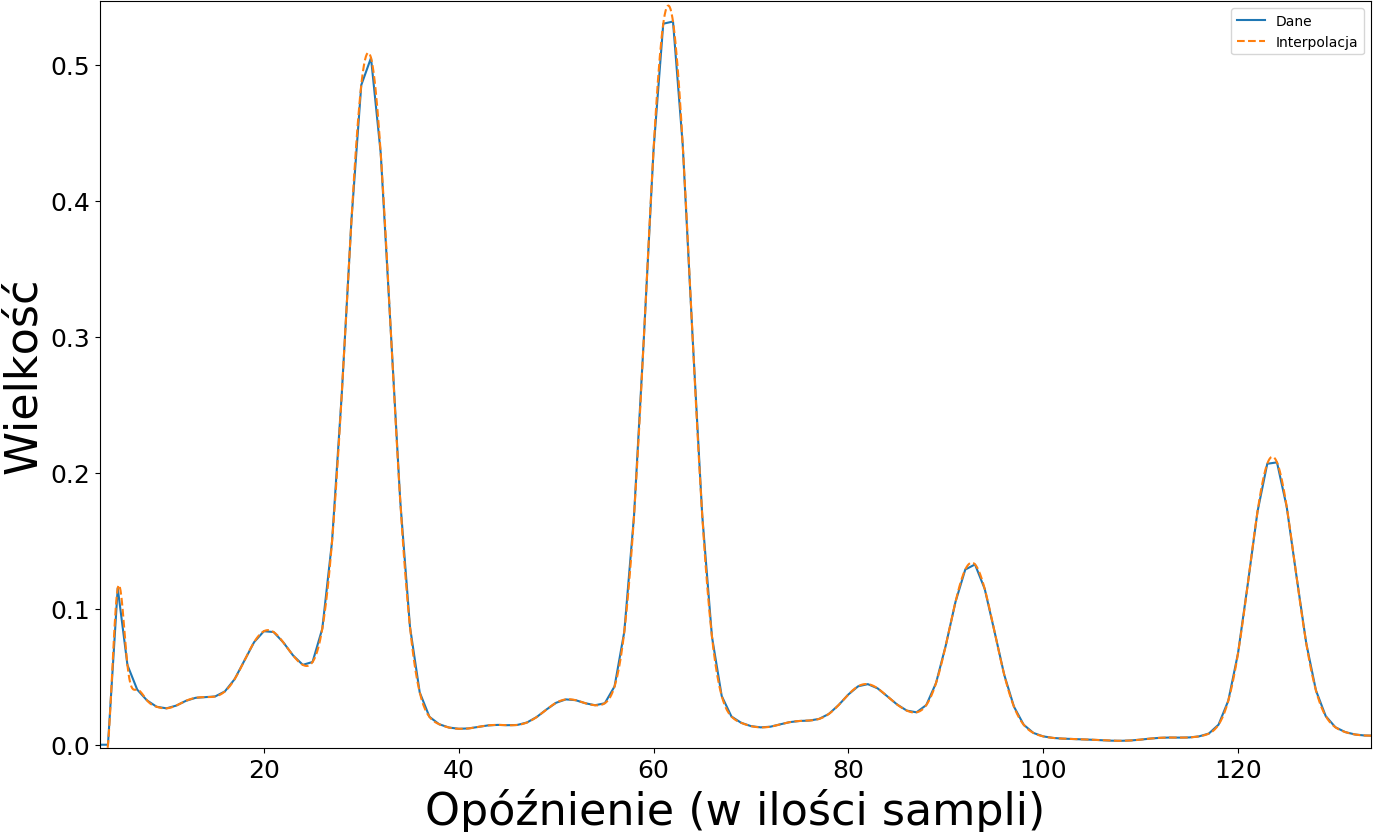
\includegraphics[width=1.\linewidth]{images/ACLOS/Interpolacja_superzoomed_cropped.png}
    \caption{Wykres (c) w przybliżeniu}
  \end{subfigure}
  \caption{Wynik ACLOS na na ,,Odzie do radości'' IX symfonii Beethovena zagranej monofonicznie na pianinie. Użyto okno Hanna o długości 2048 sampli z odstępami długości 512 sampli. Wykresy (c) i (d) przedstawiają wynik równania \ref{eq:Aclos:ACf} na tym samym oknie po zastosowaniu lifteringu. Wykresy wygenerowane przy pomocy implementacji opisanej w sekcji \ref{sec:impl:alg:aclos}.}
  \label{fig:aclos:results}
\end{figure}

Algorytm ACLOS po wyliczeniu wektora autokorelacji dla danego okna zakłada wyznaczenie F0 na podstawie maksymalnego wyniku \ref{eq:Aclos:ACf}. Szerokość pasma pojedyńczego spektralnego komponentu zależne jest od przyjętej długości okna, a pasmo to jest zakresem, w którym znajduje się znalezione F0. Autorzy używają interpolacji wokół wartości wyznaczonej przez autokorelacje co w rezultacie umożliwia uzyskanie większej dokładności wyznaczonej częstotliwości fundamentalnej. Możliwości użycia autokorelacji w metodykach wykrywania F0 zostały już pokazane między innymi w pracy \cite[1046-1047]{Transcription:Suzuki:EstimationOfMistunedFrequency}.


Wyniki ACLOS w wyznaczaniu F0 są podobne do tych, wyznaczonych przez metodę Cepstrum (\ref{sec:f0:ceps}) co można zaobserwować na rysunku \ref{fig:aclos:results}. Większa niedokładność na początku kolejnych wysokości jest spowodowana charakterystyką użytego pianina, którego barwa podczas narastania amplitudy dźwięku jest chwiejna. ACLOS jest uważane za metodę bardziej odporną na szum w analizowanym sygnale niż metoda Cepstrum \cite{Transcription:Kunieda:Aclos}.

\clearpage
\subsection{Estymacja wielotonowa}\label{sec:MultiPitch}
Ten rozdział skupia się na opisaniu metod estymacji składowej fundamentalnej w sygnale akustycznym polifonicznym. polifoniczny sygnał to taki, w którym występują co najmniej dwa dźwięki w tym samym czasie. Problem ten jest znacznie bardziej skomplikowany od wyznaczania pojedyńczego F0 opisanego w \ref{sec:f0}. Wiele z własności sygnałów akustycznych, jak periodyczność czy rozróżnialna barwa nie są wystarczające w celach transkrypcji wielotonowej, ponieważ nakładające się na siebie wysokości dźwięków mieszają miedzy sobą również ich cechy.

Współczesna muzyka zachodnia jest w mocnym stopniu ustrukturyzowana zarówno w domenie czasu jak i częstotliwości. Tempo i rytm, w którym dany utwór jest grany, jest informacją zawartą w domenie czasu. Dzięki wzorcom, które są zachowywane w muzyce, można te informacje wydobyć. W domenie częstotliwości natomiast widoczne są zależności pomiędzy poszczególnymi wysokościami dźwięków. Było to już wielokrotnie udowadniane, jak na przykład w \cite[1325-1326]{Transcription:Mcintyre:OnTheOscilation}, że pojedyńczej zagranej nucie towarzyszy, poza częstotliwością fundamentalną, szereg wydźwięków. Wibracje te badane przez fizyków były dostosowywane tak, żeby pasowały do modeli normalnych. Struktura częstotliwości różni się w zależności od użytego instrumentu i sposobu w jaki została zagrana. Częstotliwość i rozmieszczenie harmonicznych jest odgórnie ustalona przez instrument i sposób w jaki zostanie zagrana nuta. Pomimo że harmoniczne zawsze posiadają pewne odchylenie od bycia w perfekcyjnej harmonii (to znaczy nie są dokłądną algebraiczną wielokrotnością częstotliwości F0, a oscylują w jej okolicy) dla konkretnego instrumentu i sposobu zagrania będą odgórnie zdefiniowane przez pewien model matematyczny \cite[1326-1327]{Transcription:Mcintyre:OnTheOscilation}. Jak opisuje Manuel Davy w \cite[203-204]{Transcription:Anssi:SignalProcessingMethods} struktura muzyki tonalnej może zostać wykorzystana do budowy modeli bayesowskich, czyli modeli matematycznych w kontekście probabilistycznym, które prowadzą do najprostszego modelu wyjaśniającego daną fale dźwiękową. Pomimo tego, że modele te wydają się naturalnym rozwiązaniem estymacji wielotonowej, ponieważ rozwiązuje problem dużej ilości parametrów w fali dźwiękowej, których nie można wyestymować beż zakładania pewnych założeń, nie są one często wykorzystywane. Wspomniana wcześniej praca \cite{Transcription:BayesianHarmonicModels} jest przykładem wykorzystania modeli bayesowskich do analizowania sygnałów muzycznych, w tym wykrywania F0.

\subsubsection{Wyniki algorytmów do sygnałów monofonicznych}\label{sec:MultiPitch:monofon}
W rozdziale \ref{sec:f0} struktura częstotliwości rozumiała była jako obraz pojedyńczej częstotliwości fundamentalnej, z którego jednoznacznie wynika, jaka wysokość dźwięku jest grana w danym momencie czasu. Duża większość muzyki jest polifoniczna i tylko momentami skomplikowane kompozycje dopuszczają się brzmienia jedynie pojedynczych nut. W takich utworach metodologie transkrypcji muzyki monofonicznej są nieefektywne.

\begin{figure}[ht]
  \begin{center}
    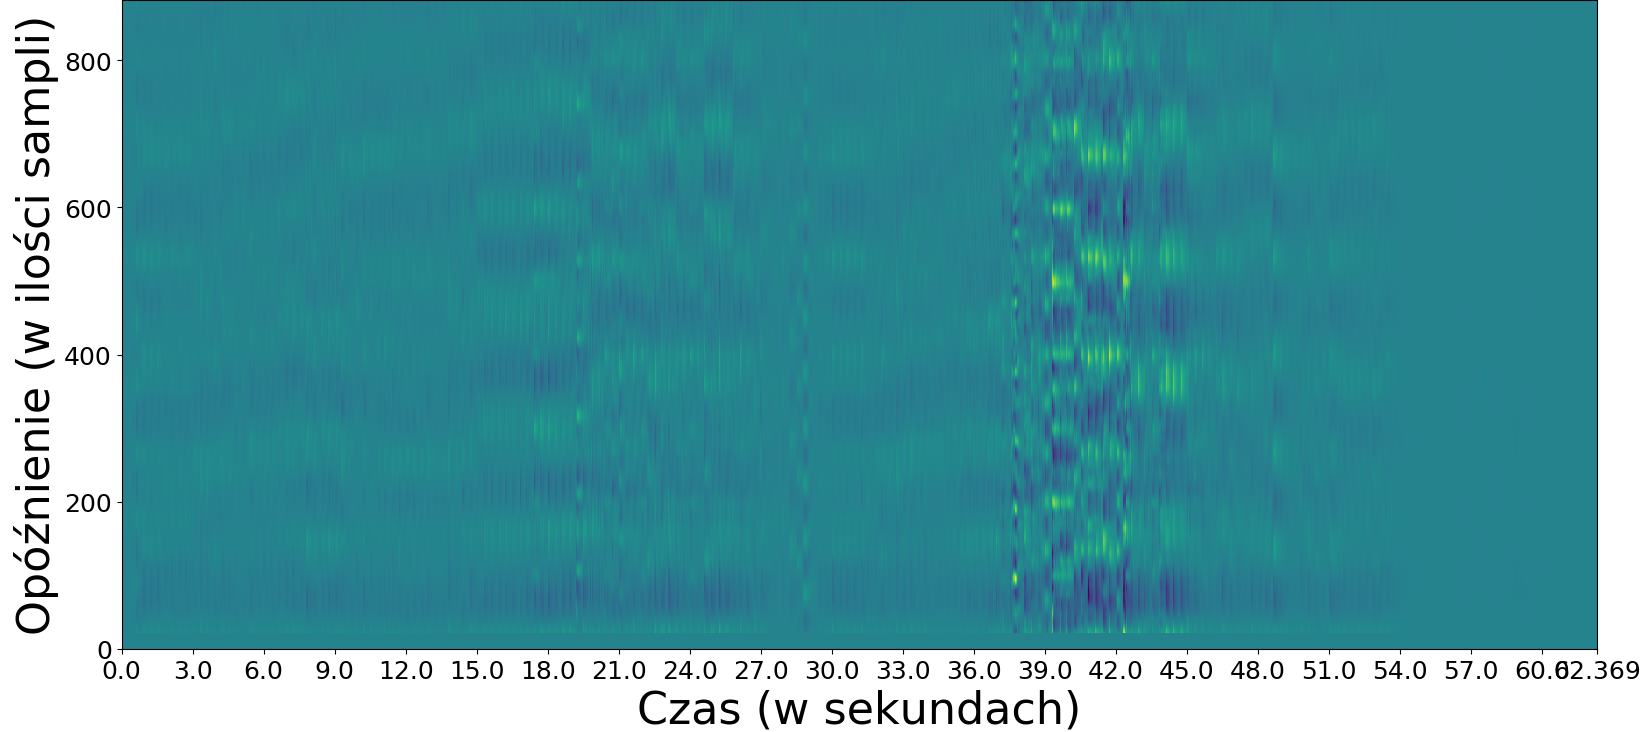
\includegraphics[scale=0.38]{images/AC/korelogram_multif0_cropped.png}
    \caption{Funkcja autokorelacji \ref{eq:AC} zastosowana na nagraniu Preludium op. 28 nr. 4 Fryderyka Chopina zagranym na pianinie w Em. Użyto okno Hanna o długości 2048 sampli z odstępami długości 2048 sampli.}
    \label{fig:multi:ac}
  \end{center}
\end{figure}

Funkcja autokorelacji w domenie czasu/mocy, jak opisana w sekcji \ref{sec:f0:ac} polegała na znalezieniu powtarzalności w fali dźwiękowej. Ta cykliczność była bezpośrednim efektem periodyczności pojedyńczych dźwięków. Gdy w tym samym czasie granych jest więcej nut, nawet na pojedyńczym instrumencie, AC nie jest w stanie odróżnić ich od siebie. Na rysunku \ref{fig:multi:ac} przedstawiony jest korelogram, wygenerowany analogicznie do korelogramu na \ref{fig:ACResults:corr} z tą różnicą, że sygnał bazowy jest w tym przypadku polifoniczny. Rezultat jest nieczytelny i nie można na jego podstawie wnioskować żadnej z dźwięków granych w utworze.

\begin{figure}[ht]
  \begin{subfigure}{1.\textwidth}
    \centering
    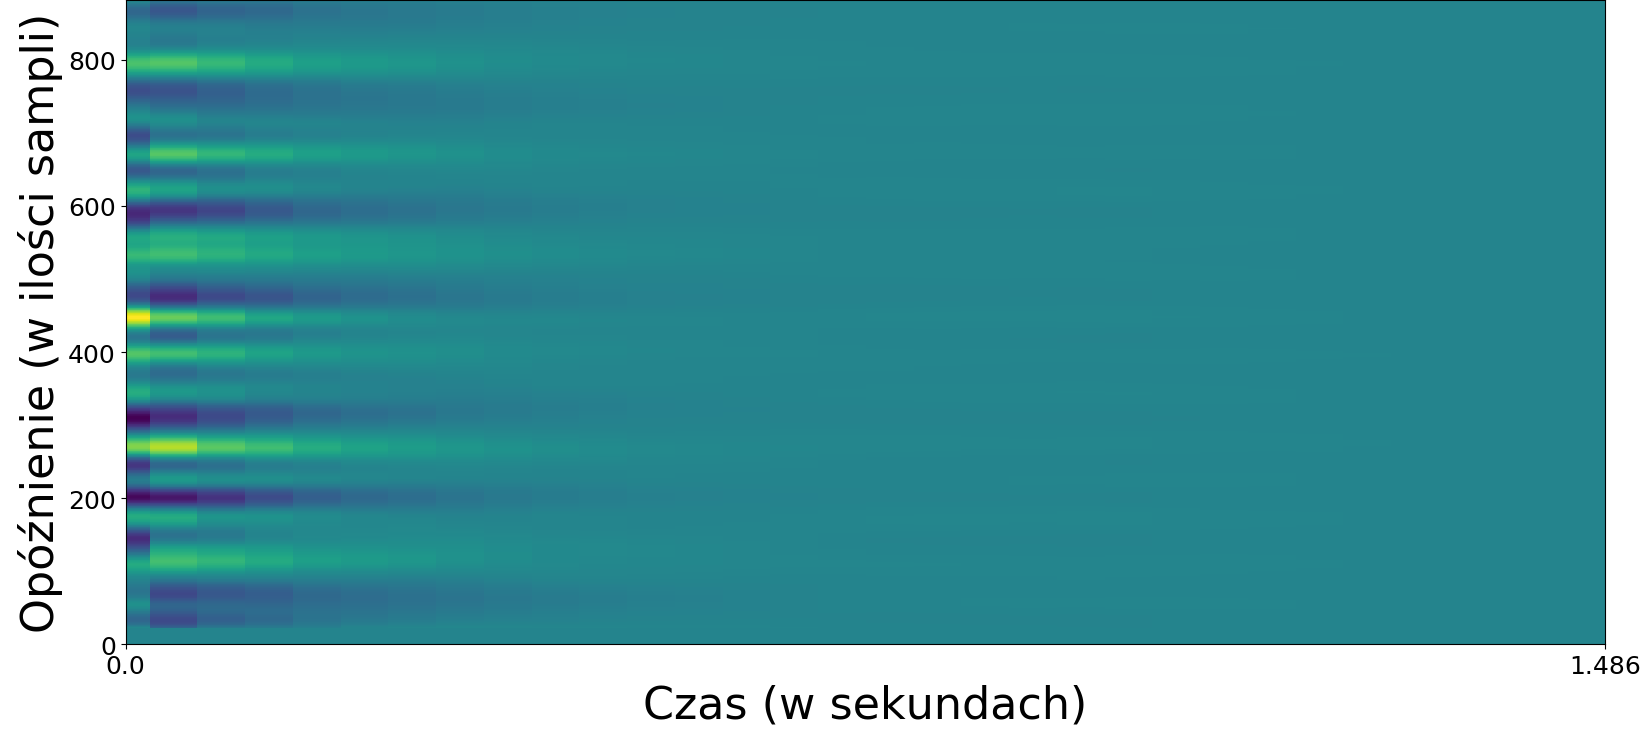
\includegraphics[width=.49\linewidth]{images/Em/Corelogram_cropped.png}
    \caption{Korelogram}
  \end{subfigure}
  \newline
  \begin{subfigure}{0.5\textwidth}
    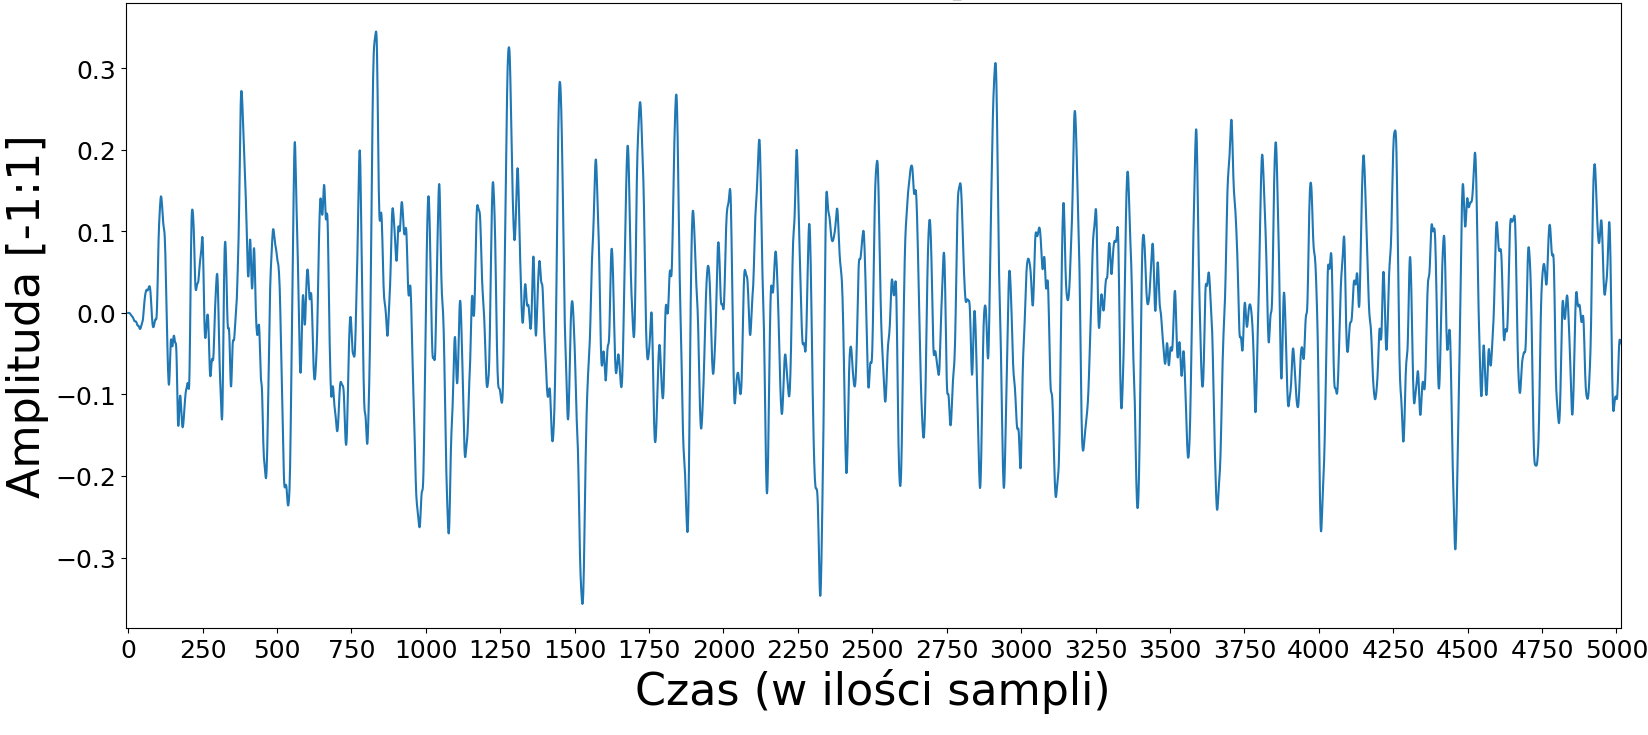
\includegraphics[width=1.\linewidth]{images/Em/waveform_zoom_samples_cropped.png}
    \caption{Sygnał fali dźwiękowej w przybliżeniu}
  \end{subfigure}
  \begin{subfigure}{0.49\textwidth}
    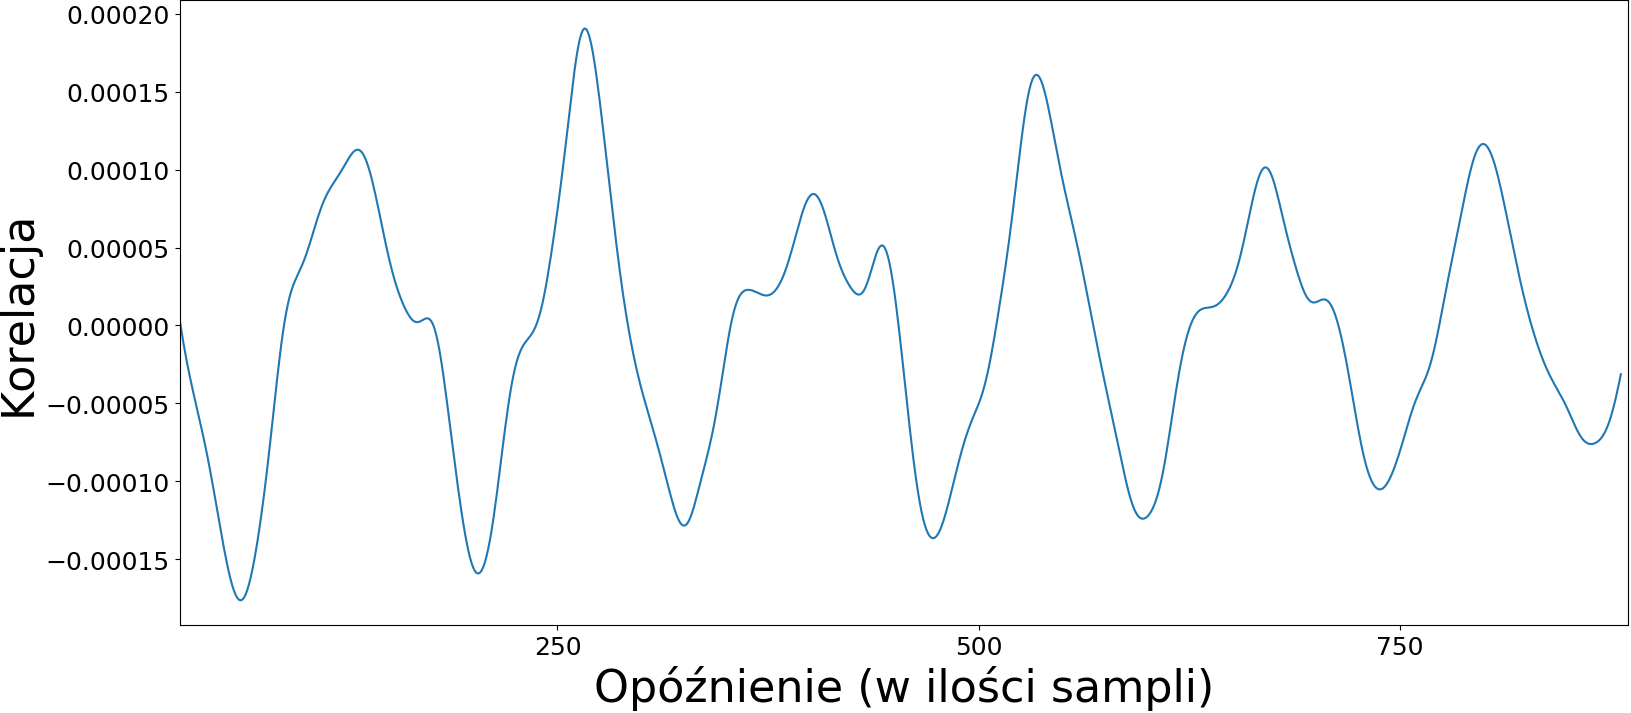
\includegraphics[width=1.\linewidth]{images/Em/corelation_cropped.png}
    \caption{Wykres autokorelacji okna danych}
  \end{subfigure}
  \caption{Wynik funkcji autokorelacji na nagraniu akordu Em zagranym na pianinie. Użyto okno Hanna o długości 2048 sampli z odstępami długości 2048 sampli. Wykresy (c) jest reprezentacją wyników AC na jedenastym oknie (próbce danych od 20480 do 22528 sampli z sygnału wejściowego).}
  \label{fig:multi:ac:em}
\end{figure}

Przyglądając się z bliska pojedyńczemu wynikowi funkcji autokorelacji jak widać na rysunku \ref{fig:multi:ac:em} można zauważyć, że piki znajdują się w nieregularnych odstępach a sama wartość funkcji korelacji nie jest bliska maksymalnej wartości. Na omawianej ilustracji grany jest akord E-mol 3, czyli dokładnie dźwięki E3, G3 i B3, którym odpowiadają częstotliwości F0 odpowiednio 164.81, 196.00 i 246.94 Hz. Na badanym oknie korelacji najwyższym pik jest w miejscu o przesunięciu 266, czyli najsilniejsza hipotezą co do F0 byłaby częstotliwość 165,8 Hz (zgodnie ze wzorem \ref{eq:AC:hz} w badanym przypadku częstotliwość wyliczana jest poprzez $44100 / 266 \approx 165,8$), co jest wartością najbliższą do częstotliwości dźwięku E3. Najniższa nuta w akordzie nazywana jest bazową, i to ona jest najbardziej charakterystyczna dla ludzkiego ucha. Z racji tego, że ma ona najniższą częstotliwość, ma też najwyższą amplitudę (z reguły im wyższa częstotliwość tym niższa amplituda), co daje wyższą szanse na znalezienie tych nut w dźwięku przy wykorzystaniu funkcji autokorelacji w domenie czasu. Drugi pik pod względem rezultatu autokorelacji jest dla przesunięcia równego 534, co odpowiada częstotliwości równej 52,6 Hz. Ta częstotliwość nie jest częścią granego dźwięku, nie jest również żadna z jej wielokrotności.

\begin{figure}[ht]
  \begin{center}
    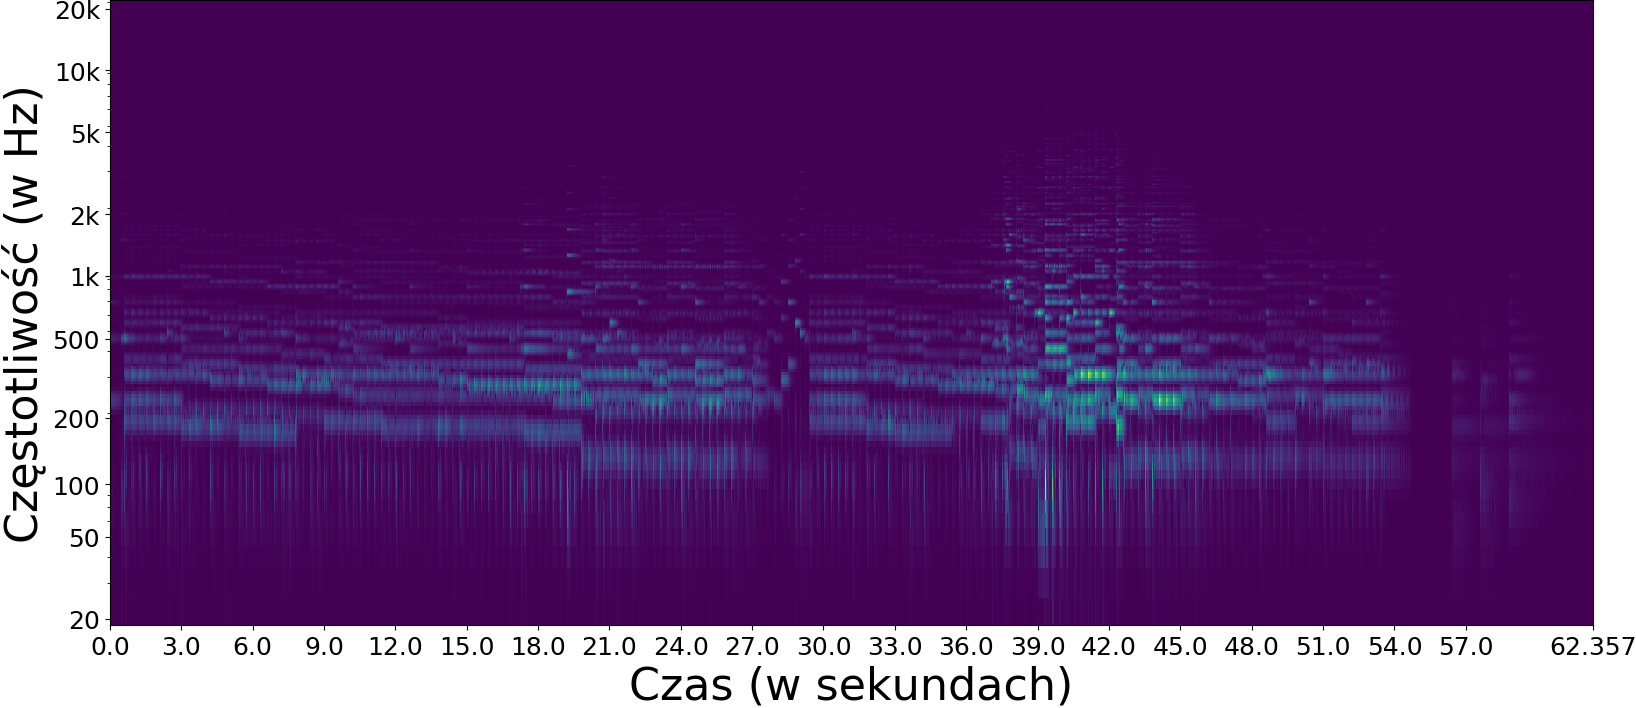
\includegraphics[scale=0.38]{images/Spectrogram/spectrogram_multi_2048_512_cropped.png}
    \caption{Spektrogram nagrania Preludium op. 28 nr. 4 Fryderyka Chopina zagranym na pianinie w Em. Użyto okno Hanna o długości 2048 sampli, marginesem zer o długości 2048 i z odstępami długości 512 sampli.}
    \label{fig:multi:spectrogram}
  \end{center}
\end{figure}

Algorytmy operujące na dziedzinie częstotliwości mają dużo większe powodzenie w wykrywaniu równoległych F0, jednak algorytmika stojąca za tymi metodami jest dużo bardziej skomplikowana niż w przypadku monofonicznych utworów ze względu na dużo bardziej skomplikowane widma. Spektrogram sygnałów polifonicznych nie jest tak wyraźnym wskaźnikiem jak był w przypadku monofonicznym. Częstotliwości harmonicznych mogą się na siebie nakładać, zniekształcając ich cykliczność jak i modulując wyraźność formantów.


Widma poszczególnych dźwięków nakładają się na siebie, wzmacniając pewne częstotliwości, a inne wytłumiając. Przykład takiego zjawiska można zaobserwować na rysunku \ref{fig:multi:spectra:partials}. Nagranie akordu Em3 nagranego na pianinie widać linią ciągłą, natomiast pojedyńczo nagrane dźwięki E3, G3 oraz B3 są przedstawione jako osobne krzywe. Widać na tym wykresie, że wynikowa krzywa Em żadko nakłada się dokłądnie z linią pojedyńczej nuty, a jest raczej nową strukturą z częścią cech wspólnych.

\begin{figure}[H]
  \begin{center}
    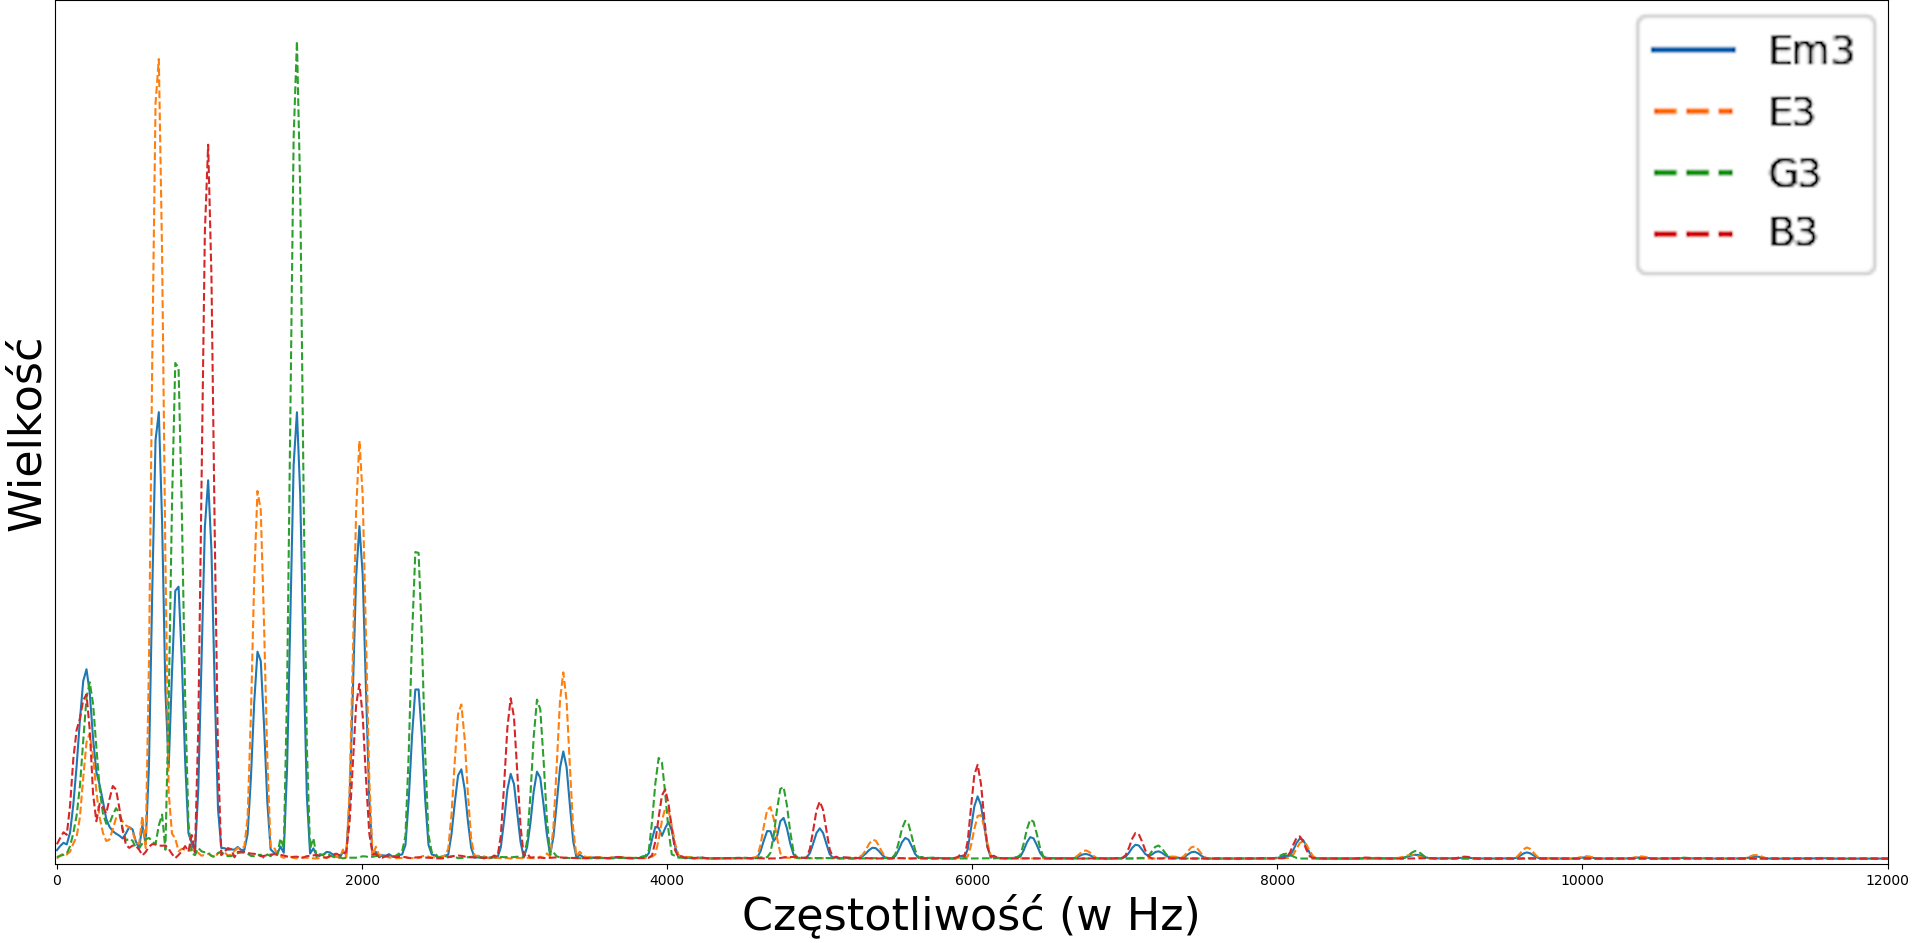
\includegraphics[scale=0.325]{images/Em/spectral_component_em3_partials_2048_512_cropped.png}
    \caption{Spektralne komponenty nagrania akordu Em zagranego na pianinie oraz trzech poszczególnych nut zagranych na tym samym pianinie nagranych osobno. Użyto okna Hanna o długości 2048 sampli i marginesu zer długości 2048.}
    \label{fig:multi:spectra:partials}
  \end{center}
\end{figure}

\begin{figure}[h]
  \begin{center}
    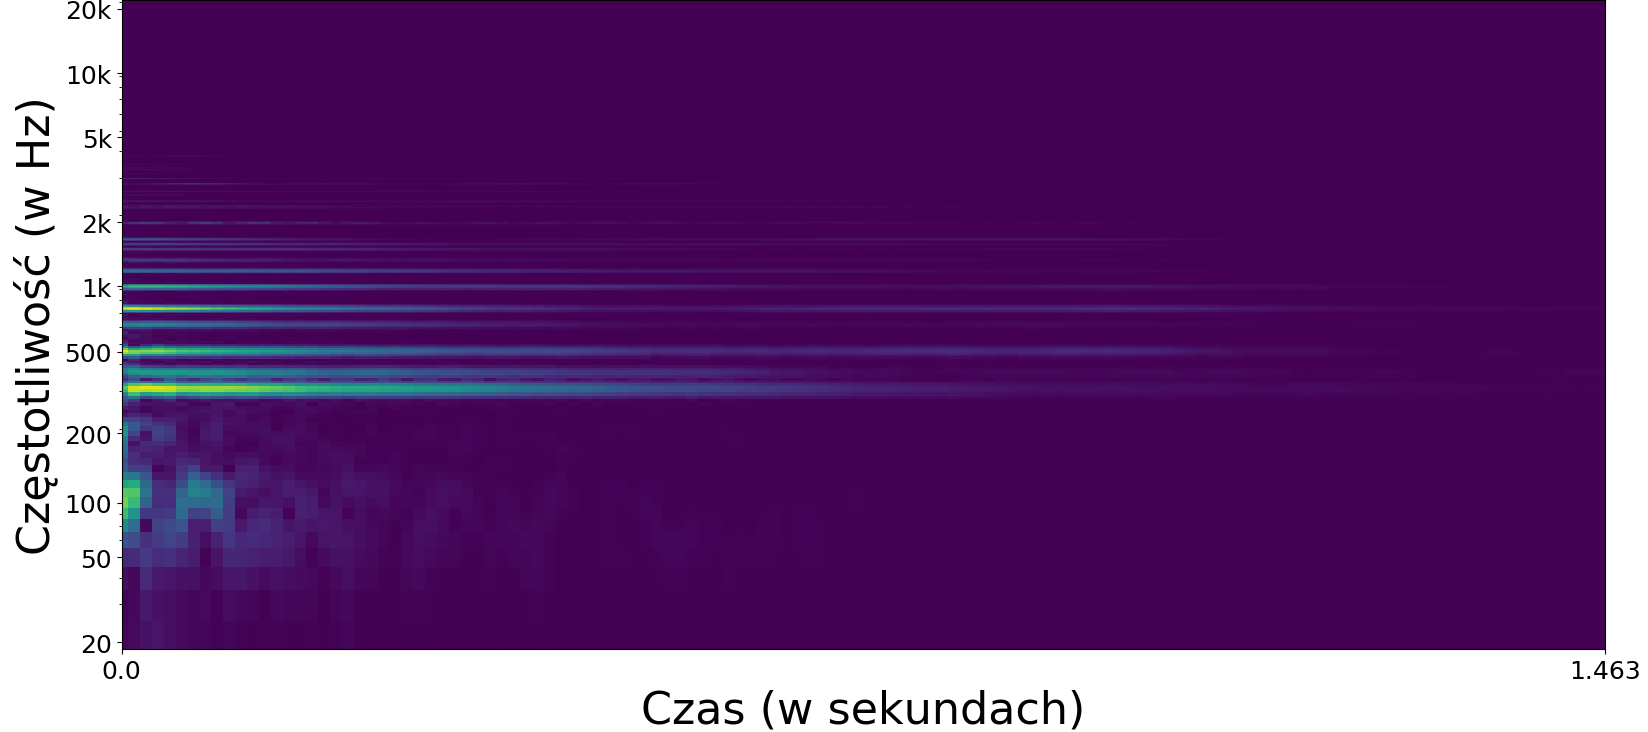
\includegraphics[scale=0.27]{images/Em/spectrogram_Em_2048_512_cropped.png}
    \caption{Spektrogram nagrania akordu Em zagranego na pianinie. Użyto okna Hanna o długości 2048 sampli z marginesem zer długości 2048 i marginesu zer długości 2048.}
    \label{fig:multi:em:spectrogram}
  \end{center}
\end{figure}

Metody cepstrum i ACLOS opisane w sekcjach \ref{sec:f0:ceps} i \ref{sec:f0:aclos} są nieefektywne z powodu nakładających się na siebie dźwięków w spektrum. Echo, które wykrywa cepstrum, jest pomieszane pomiędzy dźwiękami, co mocno komplikuje wnioskowanie z tej reprezentacji. ACLOS natomiast traci pewność wyniku z tych samych powodów co funkcja autokorelacji opisana wyżej w tej sekcji. Można zaobserwować na wykresach \ref{fig:multi:ceps:estimation} i \ref{fig:multi:aclos:estimation} że oba te algorytmy wykryły F0 w okolicach dźwięku G (ACLOS około 190 Hz, co jest najbliższe dźwiękowi G3 obecnemu w sygnale, a Cepstrum około 400, co jest wielokrotnością G3). Przyglądając się rozbitemu na poszczególne spektra wykresowi \ref{fig:multi:spectra:partials} można wywnioskować, że nuta ta ma najwięcej wspólnych harmonicznych z pozostałymi, więc właśnie ona wydaje się być najsilniejsza w widmie.

\begin{figure}[h]
  \begin{subfigure}{0.5\textwidth}
    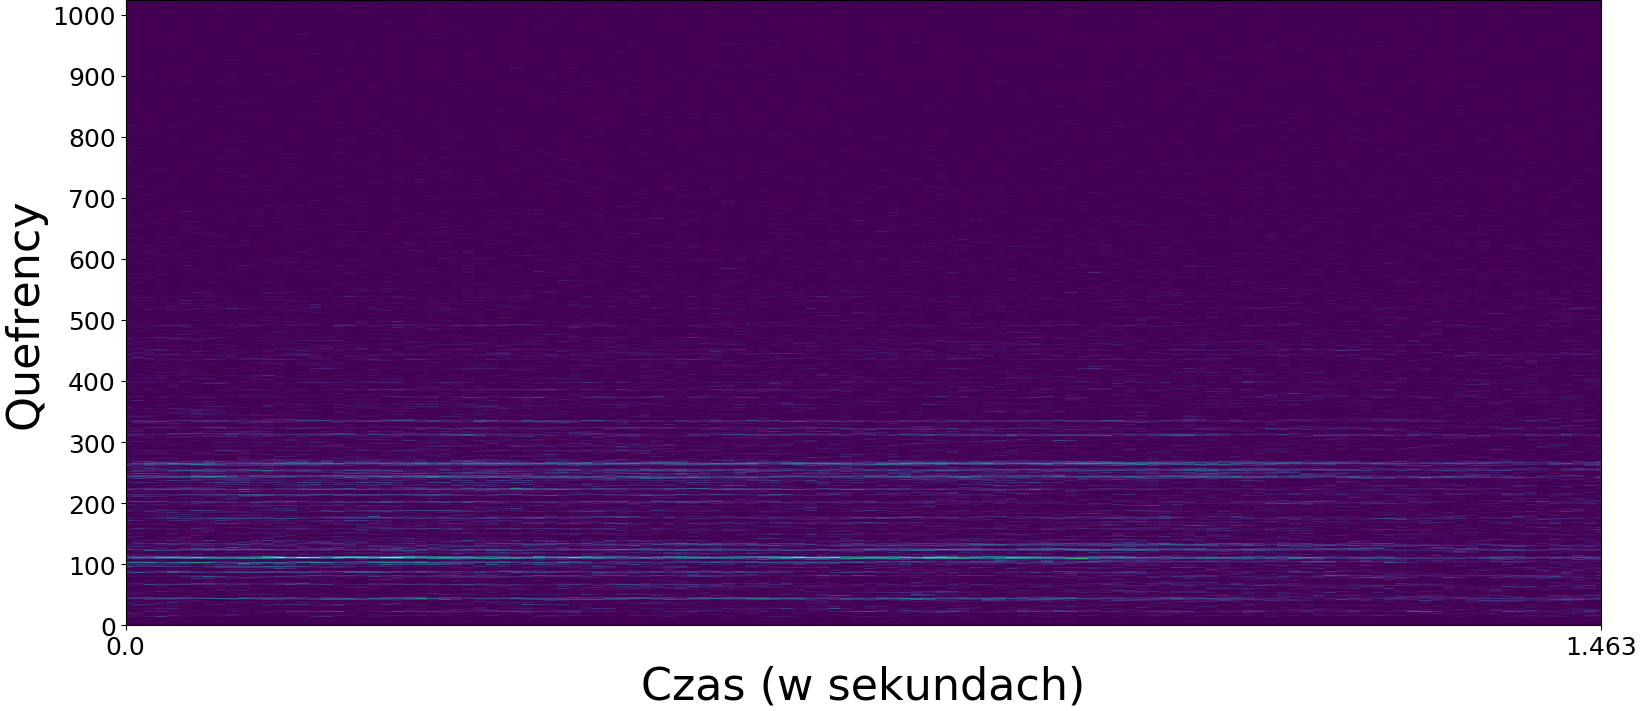
\includegraphics[width=1.\linewidth]{images/Em/cepstrogram_cropped.png}
    \caption{Cepstrogram}
  \end{subfigure}
  \begin{subfigure}{0.49\textwidth}
    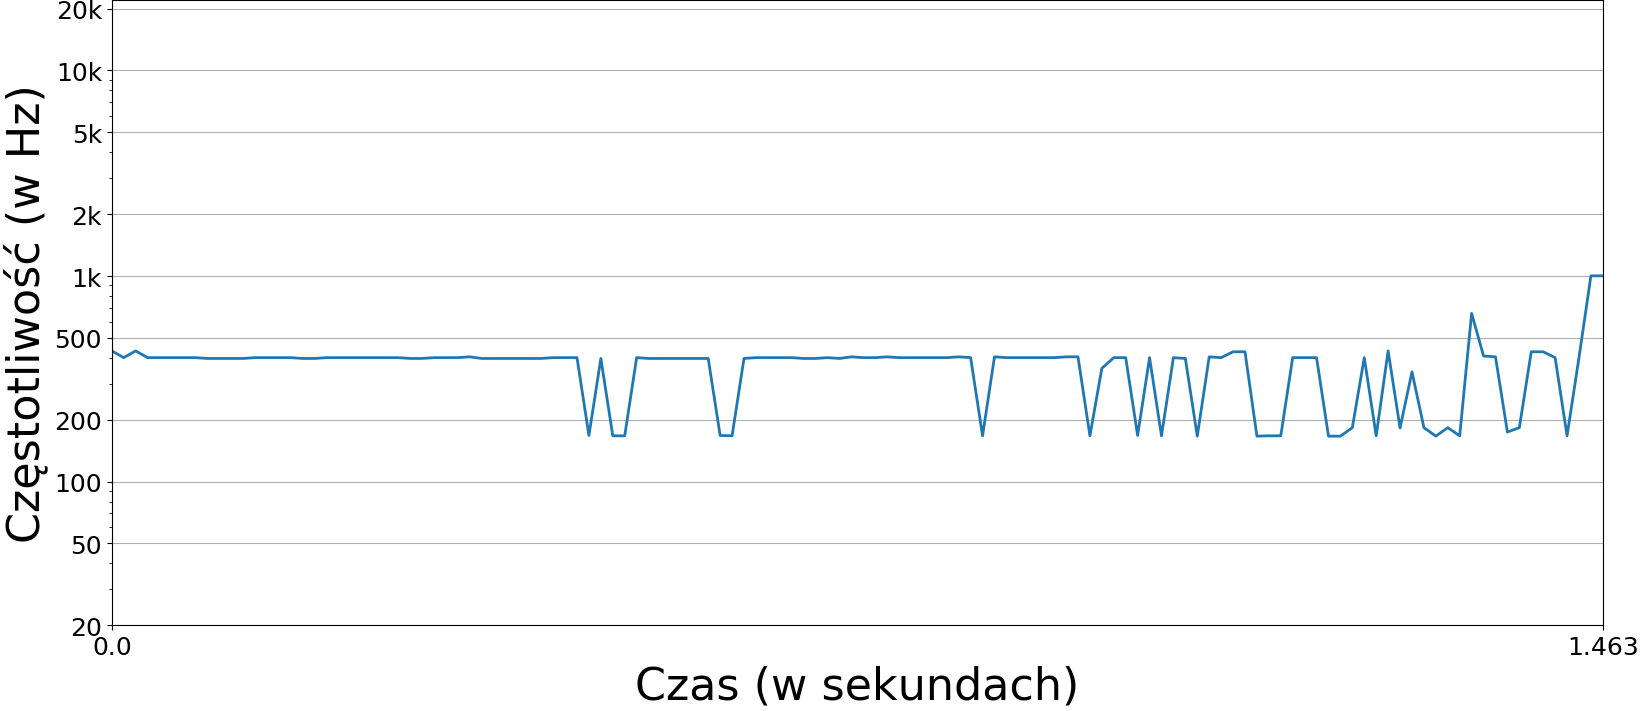
\includegraphics[width=1.\linewidth]{images/Em/cepstra_estimation_cropped.png}
    \caption{Estymacja F0}
    \label{fig:multi:ceps:estimation}
  \end{subfigure}
  \caption{Wynik cepstrum na nagraniu akordu Em zagranym na pianinie. Użyto okno Hanna o długości 2048 sampli z marginesem zer długości 2048 i odstępami długości 2048 sampli.}
  \label{fig:multi:ceps}
\end{figure}

\begin{figure}[h]
  \begin{subfigure}{0.5\textwidth}
    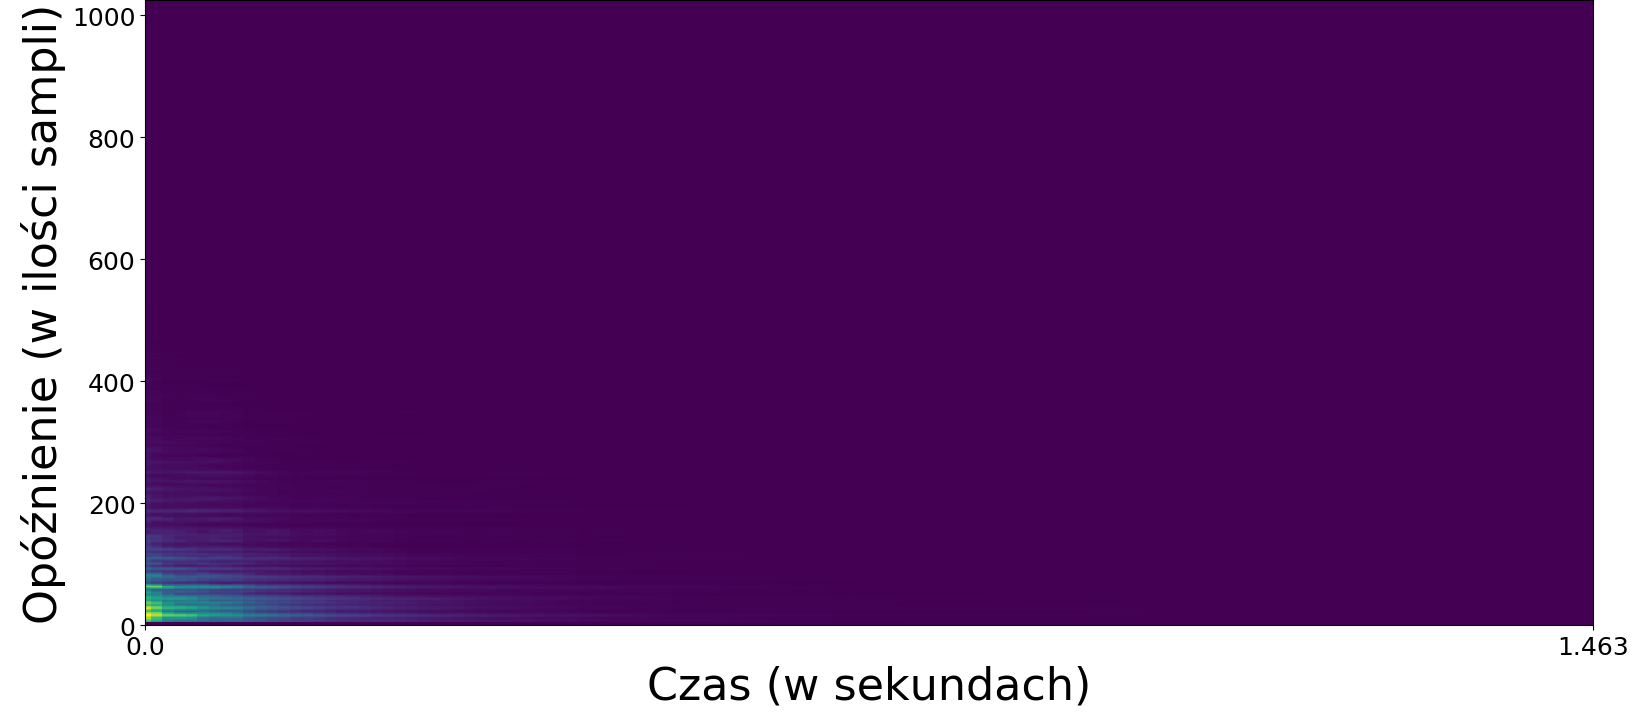
\includegraphics[width=1.\linewidth]{images/Em/Aclos_corelogram_cropped.png}
    \caption{Korelogram}
  \end{subfigure}
  \begin{subfigure}{0.49\textwidth}
    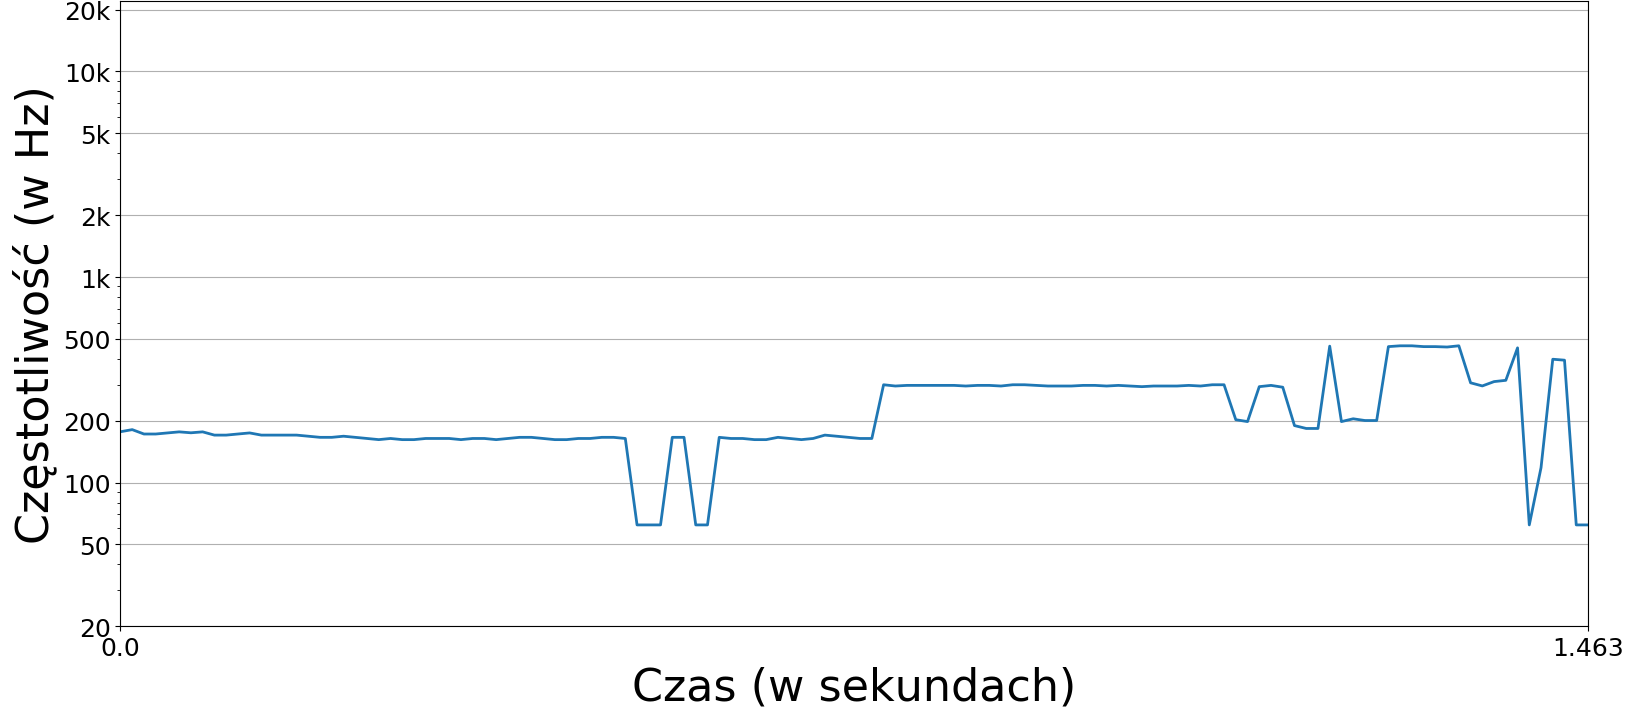
\includegraphics[width=1.\linewidth]{images/Em/Aclos_estymacja_cropped.png}
    \caption{Estymacja F0}
    \label{fig:multi:aclos:estimation}
  \end{subfigure}
  \caption{Wynik ACLOS na nagraniu akordu Em zagranym na pianinie. Użyto okno Hanna o długości 2048 sampli z marginesem zer długości 2048 i odstępami długości 2048 sampli.}
  \label{fig:multi:aclos}
\end{figure}

\subsubsection{Metody oparte o modele generatywne}
W książce \cite[203-227]{Transcription:Anssi:SignalProcessingMethods} autorzy kategoryzują metodyki przeznaczone do transkrypcji częstotliwości fundamentalnych ze względu na charakter algorytmu jaki jest użyty i są jednocześnie oparte o generatywny model fali akustycznych. Algorytmy te czerpią z modeli bayesowskich. Rozróżnili oni metody oparte o zaszumione modele sum sinusoidów, które nie brały pod uwagę zależności pomiędzy harmonicznymi (przykładem takiego podejścia jest analiza mowy opisana w \cite[744-745]{Transcription:McAulay:SinusoidalRepresentationF0}), oraz grupy modeli off-line i on-line.

Podejścia off-line charakteryzują się globalnym mierzeniem parametrów estymacji. Operują one analizując całą falę dźwiękową. Założeniem tych algorytmów jest segmentacja danych w taki sposób, że każdy z segmentów ma niezmienne wysokości granych dźwięków. Ograniczenie to wymusza na systemie transkrypcji użycia jakiejś formy wykrywania początków dźwięków. Algorytmy te bazują również na pojęciu prawdopodobieństwa, które to opisane jest matematycznym modelem wraz z gęstością. Algorytmy w tej grupie często działają według pewnych założeń co do barwy dźwięków (instrumentów czy głosu) występujących w sygnale.

Metodologie on-line są znacznie większą grupą w sensie ilości i zróżnicowaniu algorytmów. Dla każdego kroku procesu $n$ badana jest tylko część sygnału (okno) $x(n)$. Wyniki ze wcześniejszych okien są również brane pod uwagę, jako rozkład prawdopodobieństwa przejścia. Ważną różnicą pomiędzy podejściami on-line i off-line jest to, że nie potrzebują one dodatkowego mechanizmu wykrywające początki dźwięków. Autorzy w \cite[203-227]{Transcription:Anssi:SignalProcessingMethods} rozróżnili modele on-line również po tym, czy tworzony model bezpośrednio miał determinować kształt fali, czy też być modelem pośrednim w bardziej skomplikowanym systemie. Dokładniej, opisują cztery podejścia stosowane dla ogólnego przetwarzania audio, z czego wszystkie wykorzystują cechę równomiernego rozłożenia harmonicznych akustycznej fali dźwiękowej. W tej sekcji przybliżona jest metoda Yeh'a i Röbel'a dotycząca automatycznej transkrypcji polifonicznego sygnału fonicznego \cite{Transcription:Yeh:JointEvaluationF0} wraz z metodologiami opartymi na harmoniczności i gładkości widma opisanymi w \cite{Transcription:Klapuri:MultipleFundamentalFrequencyEstimation} i \cite{Transcription:Pertus:Inharmonicity}.

\paragraph{Gładkość spektrum}
W swojej pracy \cite[1]{Transcription:Yeh:JointEvaluationF0} Yeh i Röbel zakładają, że polifoniczny, quasi-harmoniczny sygnał można przedstawić za pomocą poniższego wzoru:
\begin{equation}\label{eq:Yeh:signal}
y[n] = \{ \sum_{m=1}^{M}\sum_{h_m = 1}^{H_m}a_m,h_m[n]cos((1 + \delta_{m,h_m})h_m\omega_m n + \phi_m [n])\} + v[n],
\end{equation}
Gdzie $n$ jest indeksem czasu, $M$ jest liczbą źródeł dźwięków, $H_m$ jest liczbą części dla $m$-tego źródła, $\omega_m$ reprezentuje F0 źródła $m$ a $\phi_m[n]$ jest fazą. Tak zarysowany sygnał jest w dalszej kolejności analizowany w oparciu o poszczególne komponenty. Warto zwrócić uwagę, że zakłada się szum o na tyle małej amplitudzie, że możliwym jest znalezienie poszczególnych sinusoidów składowych.

Innym istotnym wzorem opisującym sygnał źródłowy jest jego reprezentacja w domenie częstotliwości. W swojej pracy Klapuri \cite[806]{Transcription:Klapuri:MultipleFundamentalFrequencyEstimation} zdefiniowała kształt spektrum takiego sygnału jako funkcję częstotliwości:
\begin{equation}\label{eq:Klapuri:spectrum}
X(k) = H(k)S(k) + N(k)
\end{equation}
gdzie $X(k)$ jest dyskretnym spektrum mocy akustycznego sygnału źródłowego, $S(k)$ jest jest spektrum mocy wibrującego systemu, którego częstotliwość fundamentalna jest mierzona, $H(k)$ jest charakterystyką środowiska w którym dźwięk został wygenerowany wraz z fizycznymi charakterystykami instrumentu, który filtruje źródło dźwięku i wszystkimi innymi czynnikami wpływający na modulacje nagrywanego sygnału, a $N(k)$ jest spektrum mocy szumu addytywnego. Proces eliminacji $H(k)$ nosi nazwę \textit{wstępne wybielanie}.

\cite{Transcription:Klapuri:MultipitchEstimationAndSeparation}

\subsubsection{Onsets and Frames}
\begin{figure}[H]
  \begin{center}
    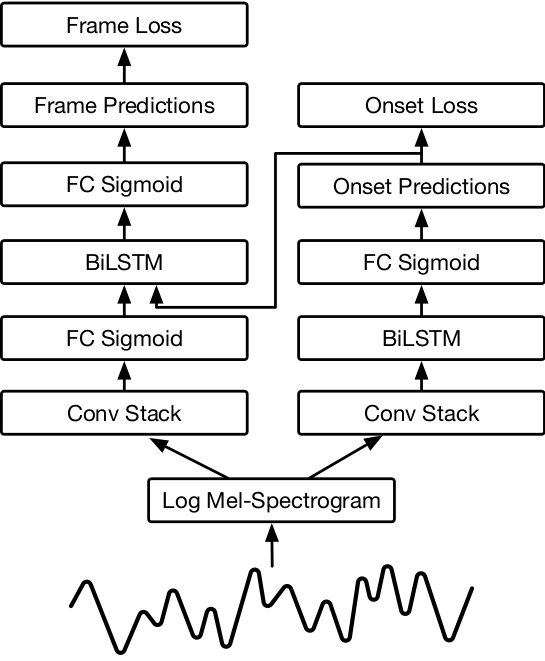
\includegraphics[scale=0.8]{images/architekturaSieciOnesetsFrames.png}
    \caption{z https://magenta.tensorflow.org/onsets-frames, diagram przedstawiający architekture sieci Onesets and Frames.}
  \end{center}
\end{figure}
\cite{DBLP:journals/corr/LuongPM15}
\todo[inline]{Czy tłumaczyć diagram?}
\todo[inline]{Do poprawy wykresy funkcji okna}
\todo[inline]{Czy mogę użyć książki której nawet nie mogę znależć on-line tylko jako referencja w innej pozycji? Który ISBN powinienem podawać, ISBN-10 czy ISBN-13? Czy istnieje jakiś stylesheet którego powinienem się trzymać? Kiedy boldować wyrazy a kiedy pisac kursywą? Wykres analizy częstotliwościowej z innej książki przyciołem o jeden wykres żeby nie zajmował tyle miejsca, czy tak można? Jak opisać implementacje i jak ma wyglądać sekcja "dodatków"?}
\newpage
% \section{Klasyfikacja muzyki}
% \cite{DBLP:journals/corr/abs-1708-03535}\cite{DBLP:journals/corr/XiongDHSSSYZ16a}
% \todo[inline]{Najprawdopodobniej rozdział do usunięcia, lub do czysto teoretycznego opisu}

% \section{Generowanie muzyki}
% \begin{figure}[H]
%   \begin{center}
%     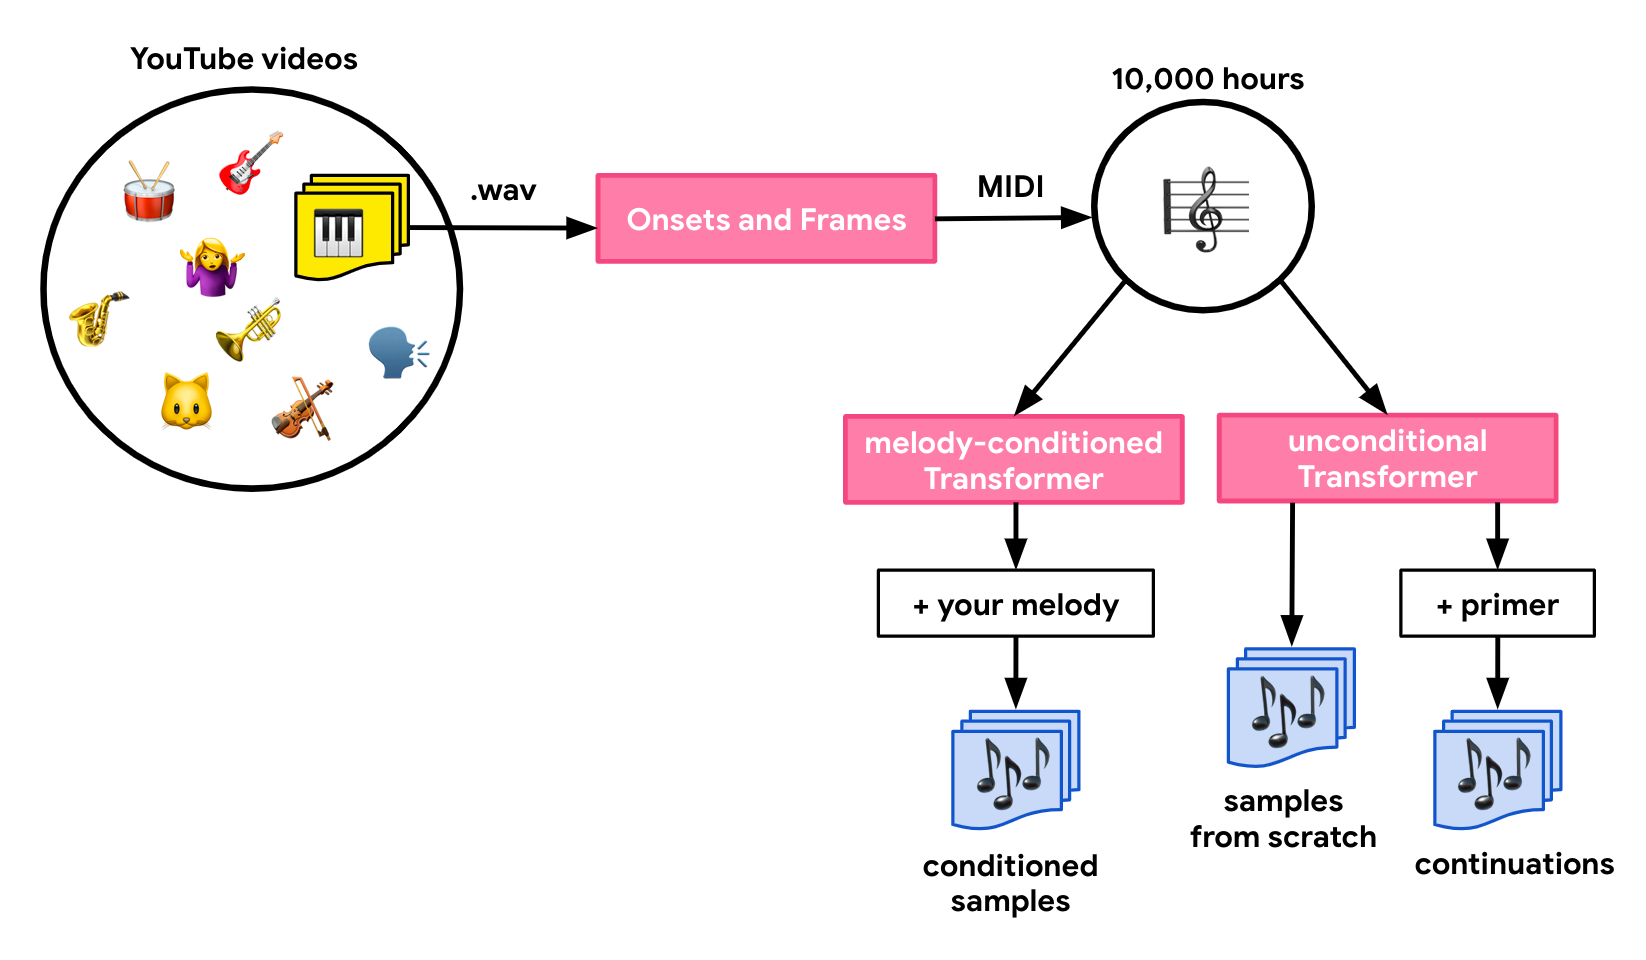
\includegraphics[scale=0.25]{images/pianoTransformerDiagram.png}
%     \caption{z https://magenta.tensorflow.org/piano-transformer, diagram przedstawiający działanie modelu Music Transformer. Do wyszukania odpowiednich klipów z YouTube został wykorzystany model AudioSet \cite{audioSet} do wyodrębnienia audio jedynie z pianinem.}
%   \end{center}
% \end{figure}
% \todo[inline]{Czy można tak używać grafiki z innych stron? Czy odniesienie do strony w bibliografi jest prawidłowe?}

% \cite{DBLP:journals/corr/abs-1809-04281}\cite{DBLP:journals/corr/VaswaniSPUJGKP17}
% \cite{DBLP:journals/corr/HuangW16}
% \cite{DBLP:journals/corr/abs-1810-12247}
% \newpage

% \section{Implementacja}
% \label{sec:implementacja}
% ~\ref{eq:midi_freq}
% \subsection{Funkcje pomocnicze}
% \newpage
% \subsection{Transpilacja}

% \subsection{Składowanie danych}
% \newpage

% \subsection{Generowanie muzyki}
% \newpage
\section{Implementacja}\label{sec:impl}

\subsection{Algorytmy}\label{sec:impl:alg}

\subsubsection{Autokorelacja}\label{sec:impl:alg:ac}
\subsubsection{Cepstrum}\label{sec:impl:alg:ceps}
\subsubsection{ACLOS}\label{sec:impl:alg:aclos}
\subsubsection{Gaussion Smoothness}\label{sec:impl:alg:specSmoothnes}
\subsubsection{Onsets And Frames}
\subsection{Interfejs GUI}
\cite{reactWDzialaniu}\cite{tsDocumentation}
\newpage
\section{Zakończenie}
\newpage


\printbibliography

\end{document}  
